\chapter{Results}
\label{cha:results}

In this chapter the results generated with the open source tool are presented.
This chapter is divided into two sections.
Section \ref{sec:results_verification} presents results from previous papers recreated using the tool.
Section \ref{sec:results_new} presents results from the newer family of models introduced in \cite{Ferrer2018a}

\section{Verification of previous results}
\label{sec:results_verification}

In this section a replication of previous results is presented.
This allows to verify the model and its implementation against previous experiments.

However, in some cases there was limited information in the original papers about the parameter used in the experiments.
In other cases, there were errors in previous papers.
In both cases, determining the correct parameter becomes a matter of trial and error.

The $\phi$ parameter was not considered in either of the papers replicated in this section, and so it is set to 0.

Section \ref{sec:results_verification_first} replicates the results from \cite{Ferrer2005a}, which correspond to the \firstmodel{} from this thesis.
Section \ref{sec:results_verification_second} replicates the results from \cite{Ferrer2003a}, corresponding to the \secondmodel{}.

\subsection{Results from the \firstmodel{} (2005)}
\label{sec:results_verification_first}

\begin{figure}
  \centering
  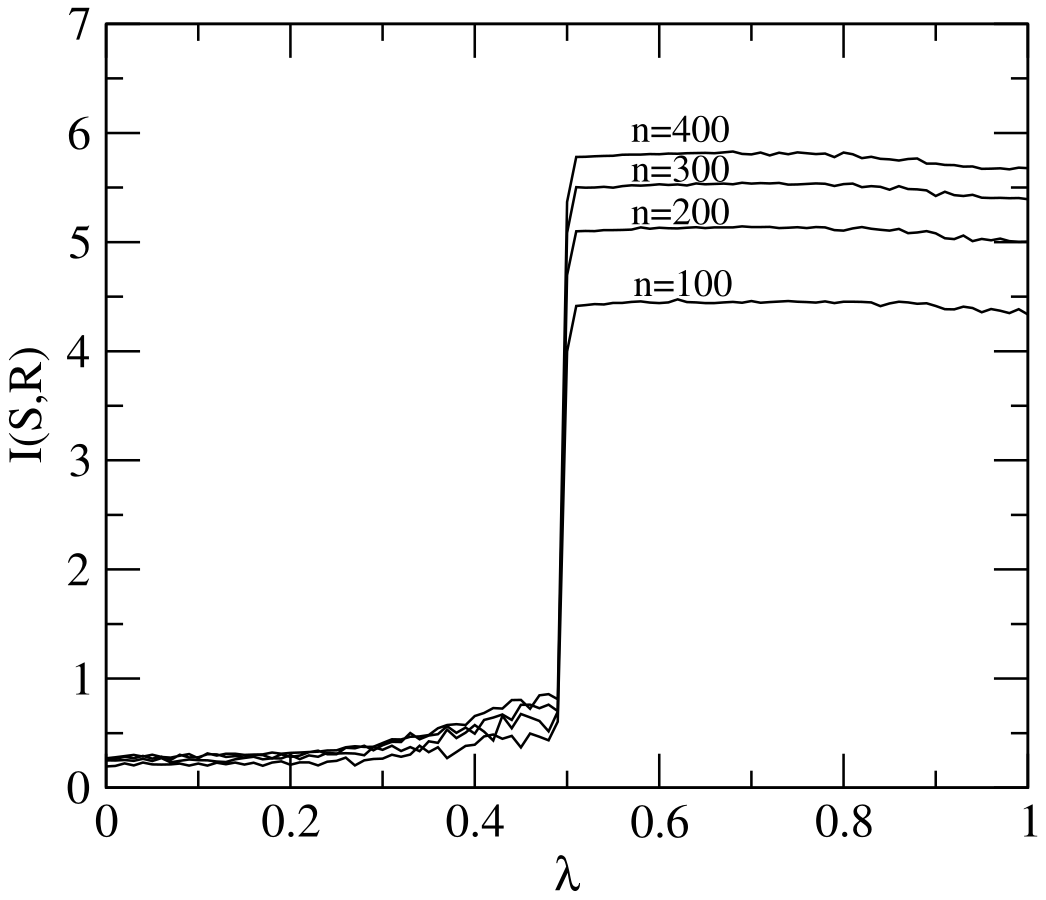
\includegraphics[width=\textwidth,height=.4\textheight,keepaspectratio]{fig2_2005_old}
  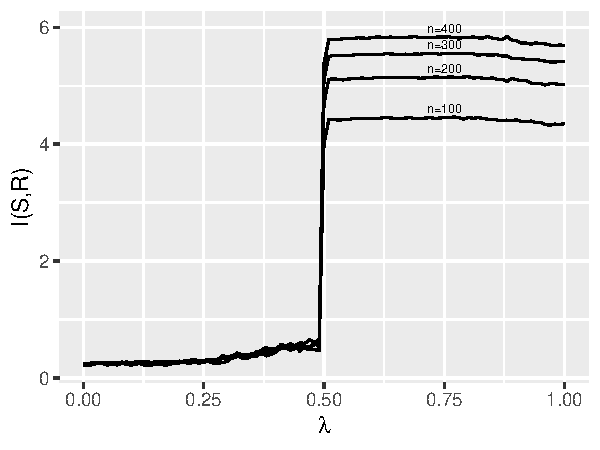
\includegraphics[width=\textwidth,height=.4\textheight,keepaspectratio]{figure2_article_EPJ_B_2005}
  \caption{
    Above: Figure 2 from \cite{Ferrer2005a}.\\
    Below: Recreation of that same figure using the open source tool created for this thesis.\\
    The mutual information $I(S,R)$ is in the $y$ axis and the $\lambda$ parameter on the $x$ axis.
    Graphs of different sizes are shown, $n=m=100$, $n=m=200$, $n=m=300$, $n=m=400$.
    Averages over 30 realizations.
    $\phi=0$, the initial graph is $G_{n,m,1/n}$, each iteration of the optimization algorithm performs 2 mutations on the graph, the weak stop condition is used to stop the optimization process, unlinked objects are allowed.
  }
  \label{fig:fig2_2005}
\end{figure}

\begin{figure}
  \centering
  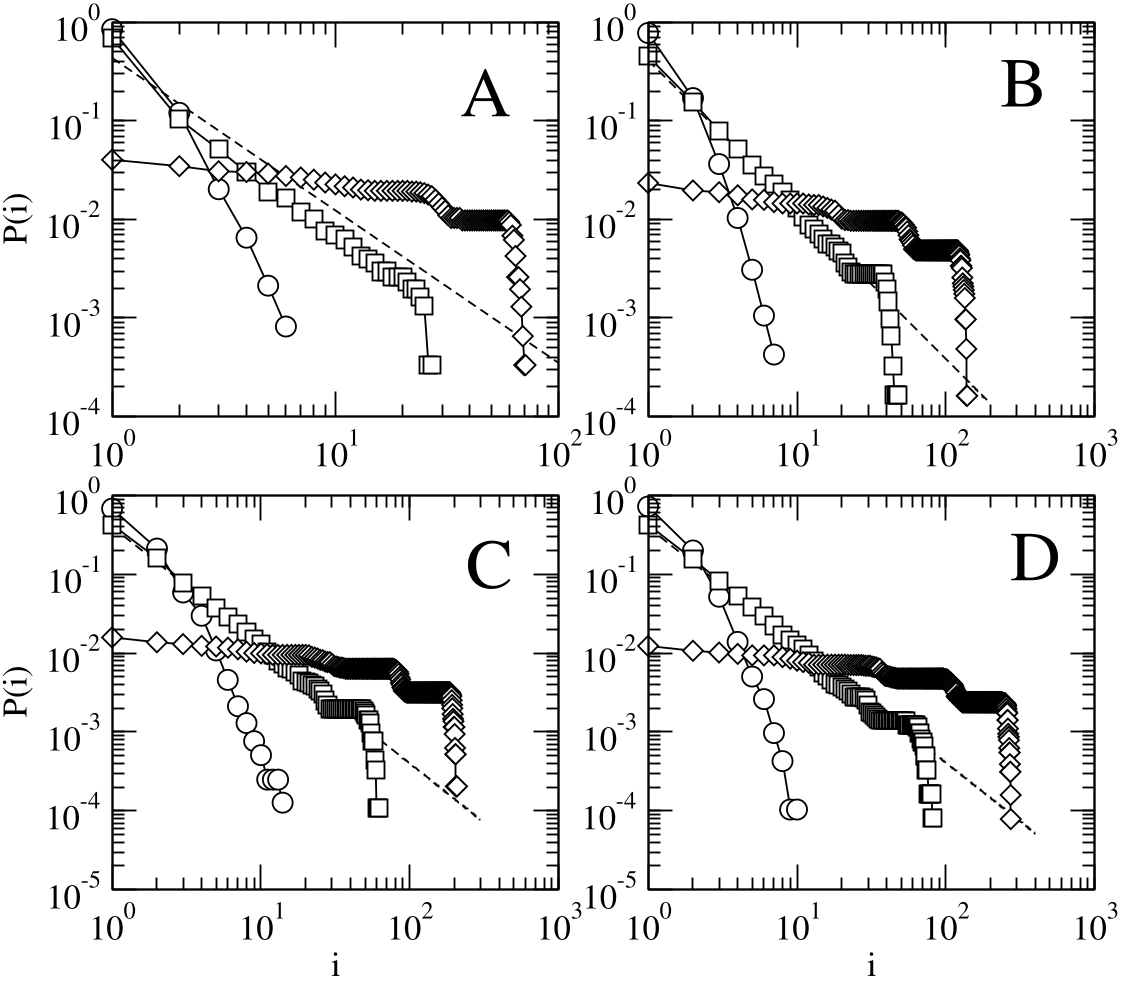
\includegraphics[width=\textwidth,height=.35\textheight,keepaspectratio]{fig3_2005_old}
  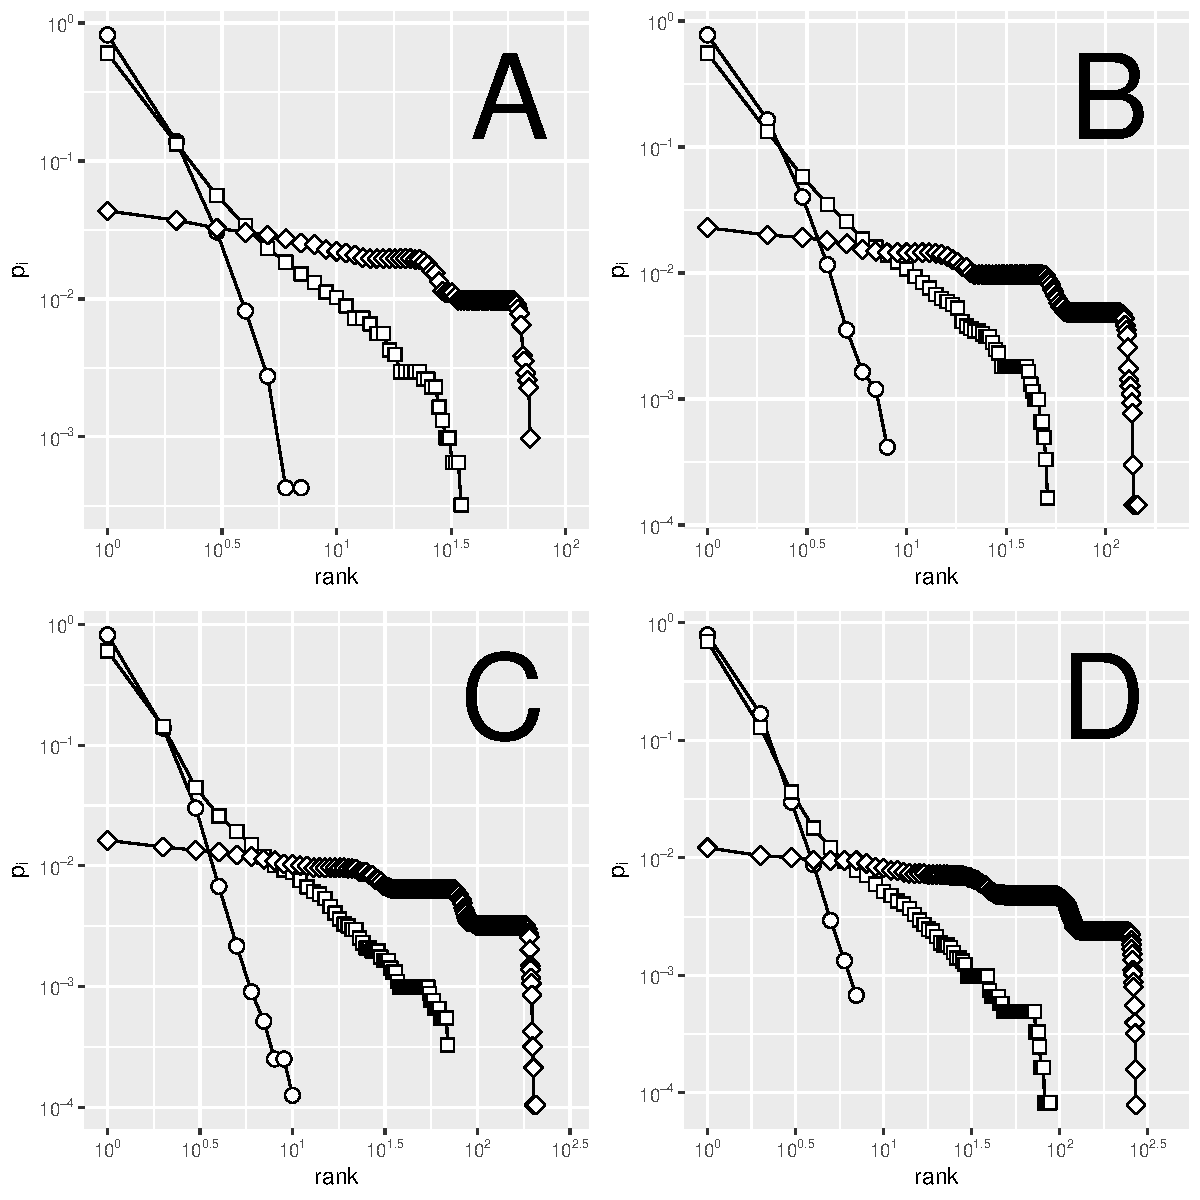
\includegraphics[width=\textwidth,height=.35\textheight,keepaspectratio]{figure3_article_EPJ_B_2005}
  \caption{
    Above: Figure 3 from \cite{Ferrer2005a}.\\
    Below: Recreation of that same figure using the open source tool created for this thesis.\\
    $P(i)$, the probability of the $i$th most frequent signal, obtained from minimum energy configurations for systems of sizes $n=m=100$ (A), $n=m=200$ (B), $n=m=300$ (C), $n=m=400$ (D).
    Four series are shown in each plot, $\lambda=0.49$ (circles), $\lambda=\lambda^*$ (squares) and $\lambda=0.5$ (diamonds) and the ideal curve for $\alpha^*$.
    Averages over 30 realizations.
    When $\lambda=\lambda^*$, $\alpha^* = 1.54$ for $n=m=100$, $\alpha^* = 1.51$ for $n=m=200$, $\alpha^* = 1.5$ for $n=m=300$ and $\alpha^* = 1.49$ for $n=m=400$.
    It was chosen that $\lambda^* = 0.4986$ for $n=m=100$, $\lambda^* = 0.4987$ for $n=m=200$, $\lambda^* = 0.4987$ for $n=m=300$, and $\lambda^* = 0.4986$ for $n=m=400$.
    Averages over 30 realizations.
    $\phi=0$, the initial graph is $G_{n,m,1/n}$, each iteration of the optimization algorithm performs 2 mutations on the graph, the weak stop condition is used to stop the optimization process, unlinked objects are allowed.
  }
  \label{fig:fig3_2005}
\end{figure}

Figure \ref{fig:fig2_2005} shows both the original Figure 2 from \cite{Ferrer2005a} and a recreation of this figure using the new tool.
Figure \ref{fig:fig3_2005} shows both the original Figure 3 from \cite{Ferrer2005a} and a recreation of this figure, also generated using the new tool.

The initial graph was not specified in \cite{Ferrer2005a} and a $G_{n,m,1/n}$ ($n=m$) graph is used in the replication.
The paper also does not specify how to stop the optimization process and so the weak stop condition (Section \ref{sec:methods_optimization}) is used.

\subsection{Results from the \secondmodel{} (2003)}
\label{sec:results_verification_second}

\begin{figure}
  \centering
  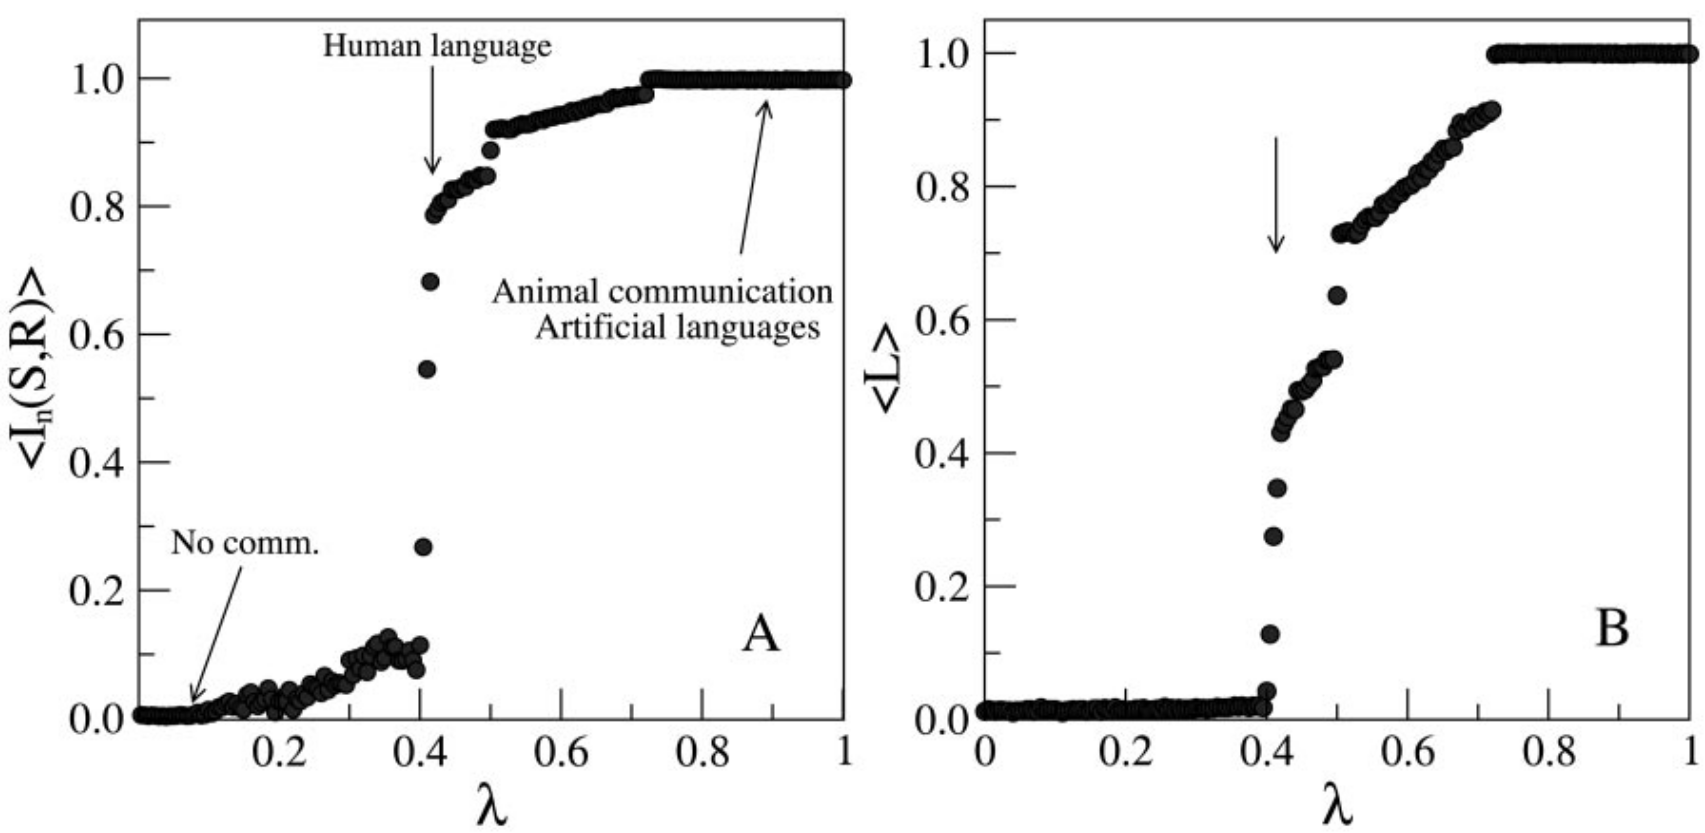
\includegraphics[width=\textwidth]{fig2_2003_old}
  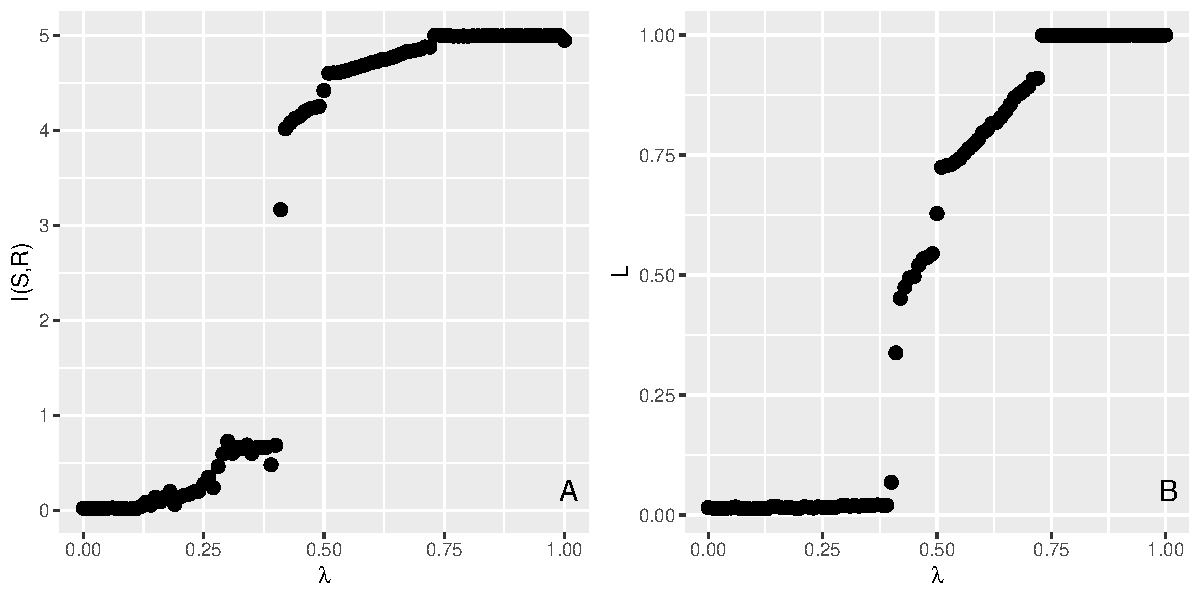
\includegraphics[width=\textwidth]{figure2_article_PNAS_2003_binom1.75}
  \caption{
    Above: Figure 2 from \cite{Ferrer2003a}\\
    Below: Recreation of that same figure using the open source tool created for this thesis.\\
    In A, $I(S,R)$ is the mutual information obtained for values of $\lambda$ between 0 and 1.
    In B, $L$ is the lexicon size obtained for values of $\lambda$ between 0 and 1.
    An abrupt change is seen for $\lambda \approx 0.41$ in both A and B.
    Averages over 30 replicas.
    $n=m=150$, $\phi=0$, unlinked objects are not allowed, $\pi$ follows a uniform distribution, 
  }
  \label{fig:fig2_2003}
\end{figure}

\begin{figure}
  \centering
  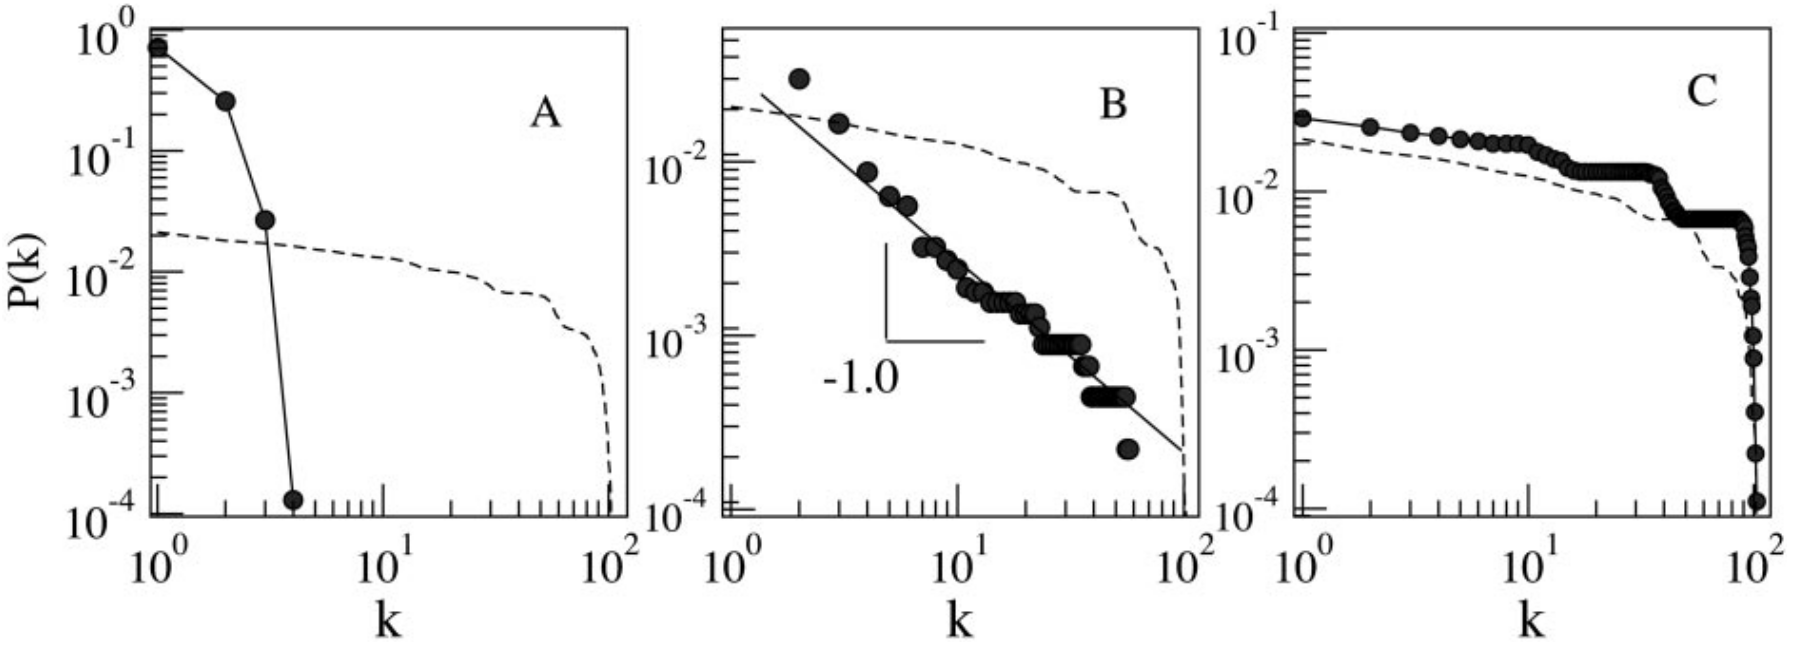
\includegraphics[width=\textwidth]{fig3_2003_old}
  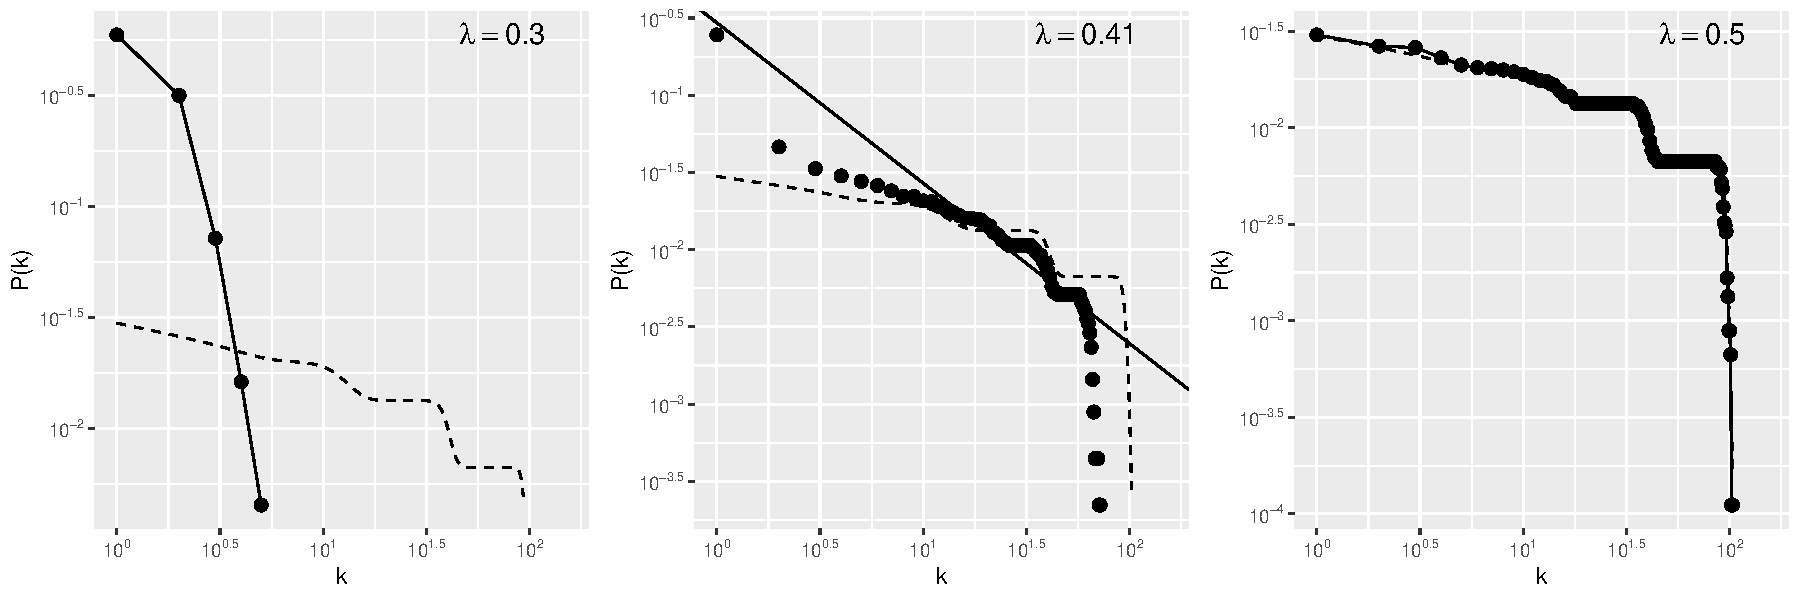
\includegraphics[width=\textwidth]{figure3_article_PNAS_2003_binom1.75}
  \caption{
    Above: Figure 3 from \cite{Ferrer2003a}\\
    Below: Recreation of that same figure using the open source tool created for this thesis.
    \\
    Normalized signal frequency $P(k)$ versus rank $k$.
    The dashed lines show the distribution obtained when from a $G_{n,m,e^*}$ graph where $e^*$ is the number of connections in these optimal configurations.
    In both cases the distribution of B is still consistent with human language, $\alpha=1$.
    Averages over 30 replicas, $n=m=150$, the initial graph is $G_{n,m,10/n}$, the number of mutations on each iteration follows a binomial distribution with average 1.75, the optimization stops after $2*n*m$ mutations that do not improve the cost function.
  }
  \label{fig:fig3_2003}
\end{figure}

Figure \ref{fig:fig2_2003} shows both the original Figure 2 from \cite{Ferrer2003a} and the recreation of this figure using the new tool.
Figure \ref{fig:fig3_2003} shows the original Figure3 from \cite{Ferrer2003a} and a recreation using the new tool.

The initial graph was specified as a $G_{n,m,\rho}$ but the value of $\rho$ was not given in the paper, a $G_{n,m,10/n}$ graph was used (that is, a value of $\rho=\frac{10}{n}$).
It is specified that the number of mutations done on each iteration of the optimization algorithm follows a binomial distribution.
However it was later found that, due to a bug in the generator of binomial numbers, the number of mutations must have been lower.
Several values were tried for the average number of binomial mutations, with 1.75 giving the best results.

\section{Results for current models}
\label{sec:results_new}

\subsection{Information Theoretic}

\subsubsection{first model, $\phi=0$}

\begin{figure}
  \centering
  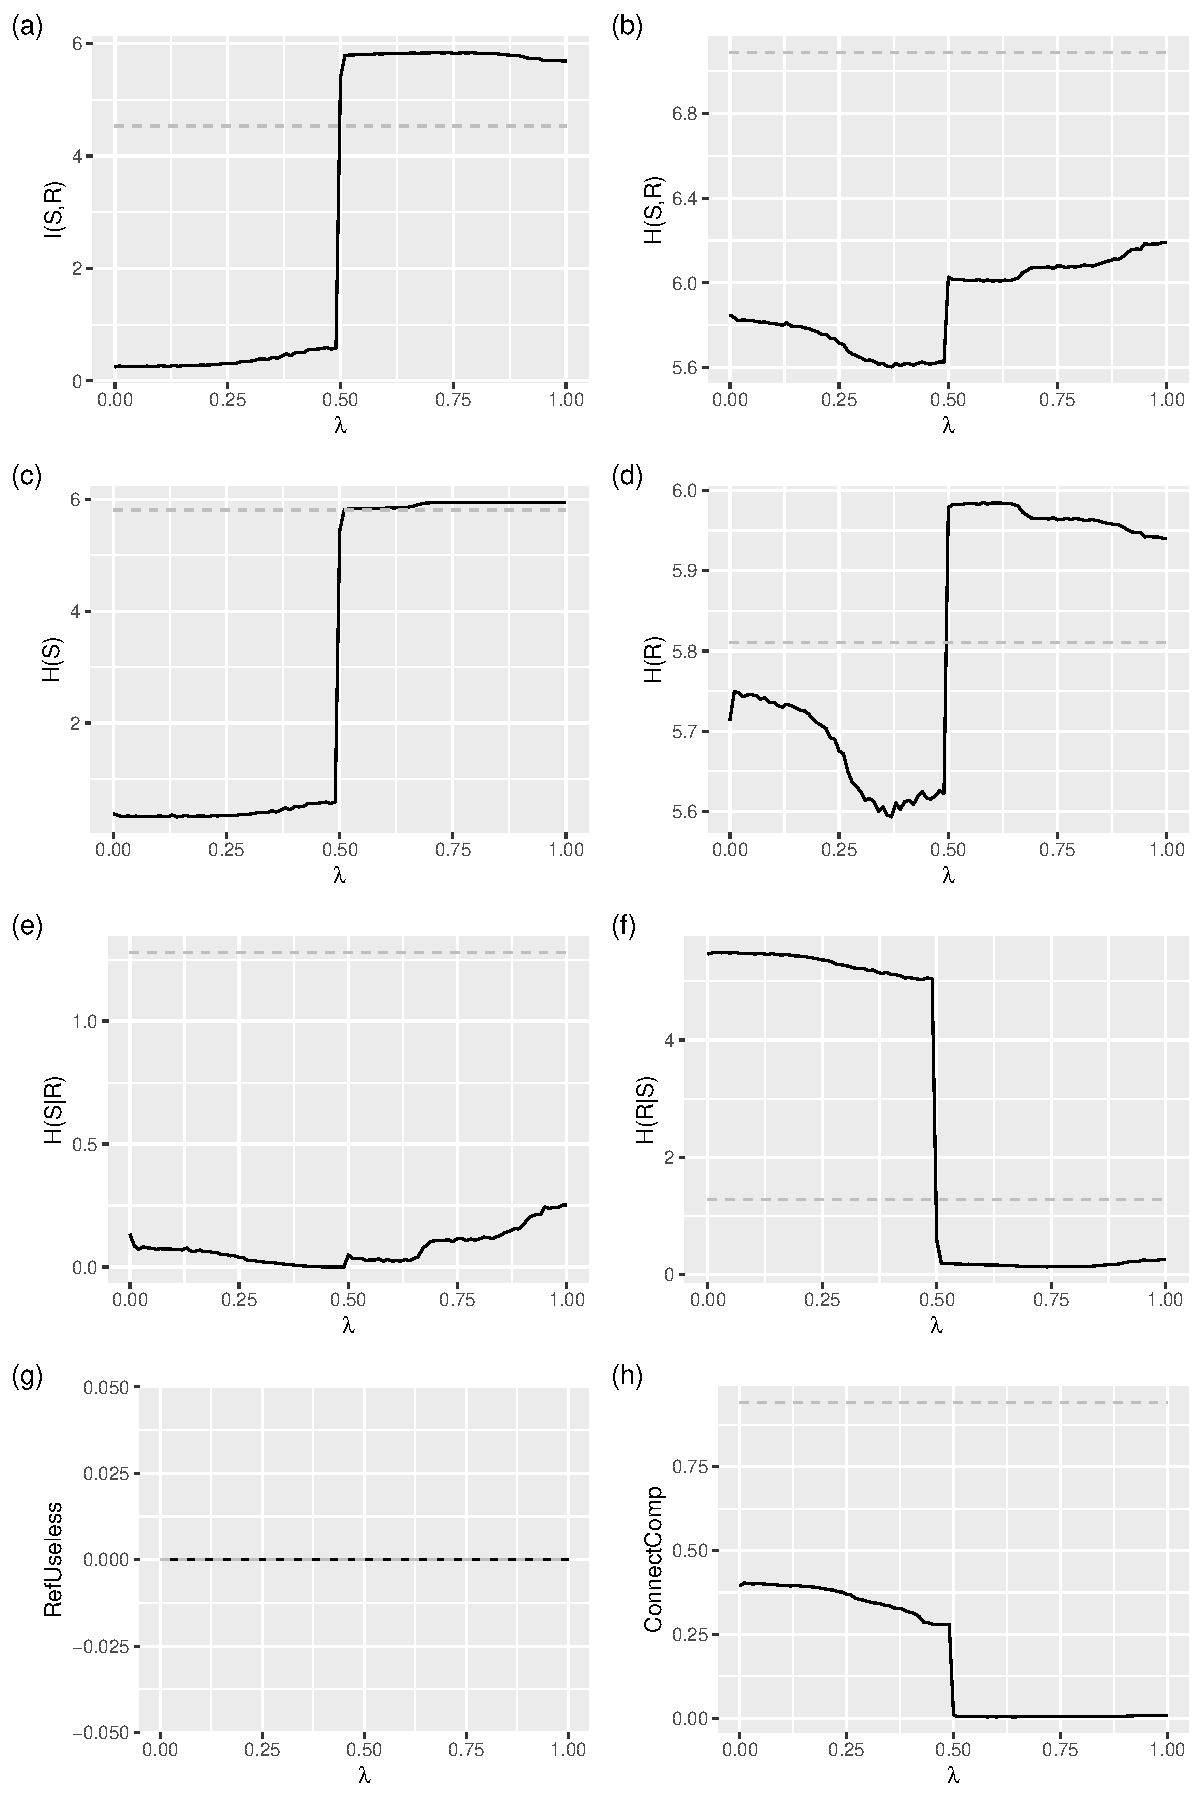
\includegraphics[width=\textwidth]{informationTheoretic_firstModel_phi0_nm400_dynamic_randomBipartite_allowUnlinked}
  \caption{a}
  \label{fig:informationTheoretic_firstModel_phi0_nm400_dynamic_randomBipartite_allowUnlinked}
\end{figure}

\begin{figure}
  \centering
  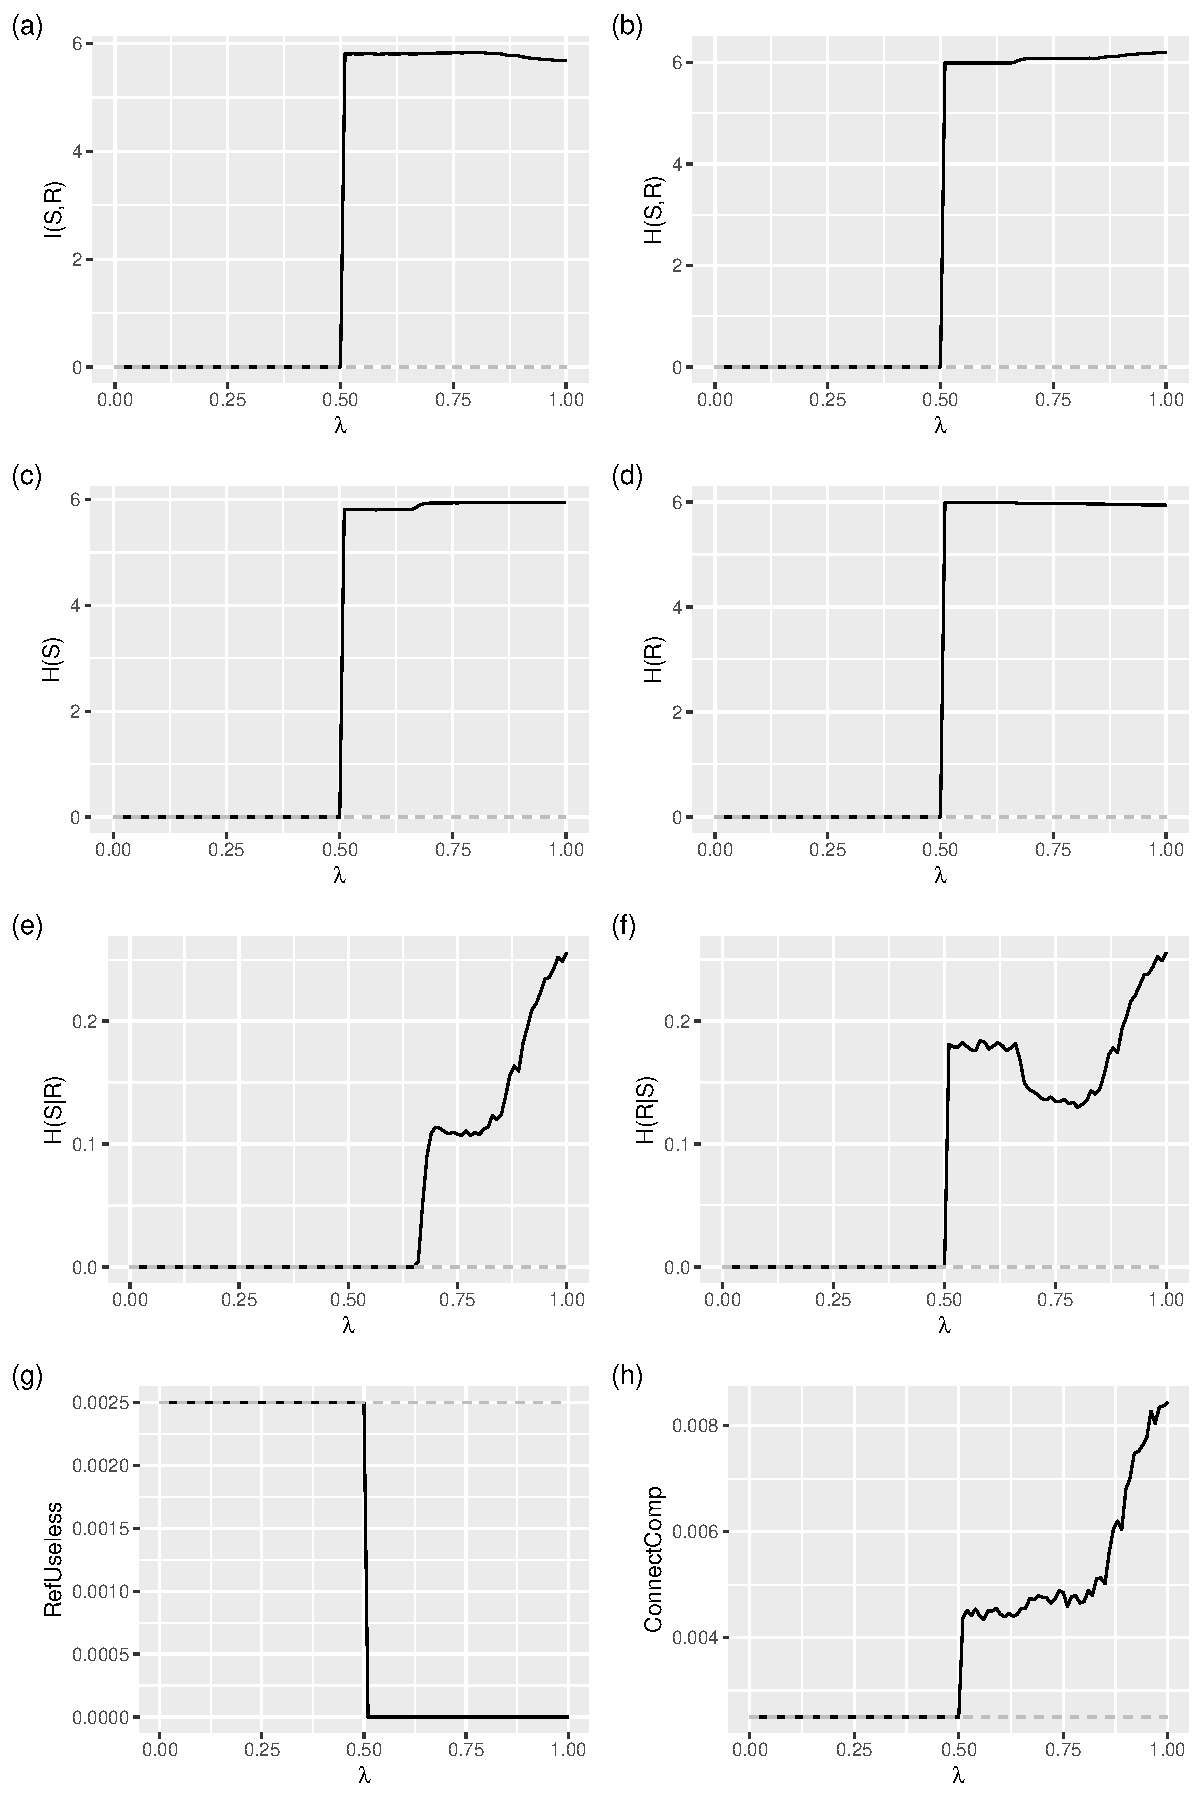
\includegraphics[width=\textwidth]{informationTheoretic_firstModel_phi0_nm400_dynamic_singleLink_allowUnlinked}
  \caption{a}
  \label{fig:informationTheoretic_firstModel_phi0_nm400_dynamic_singleLink_allowUnlinked}
\end{figure}

\begin{figure}
  \centering
  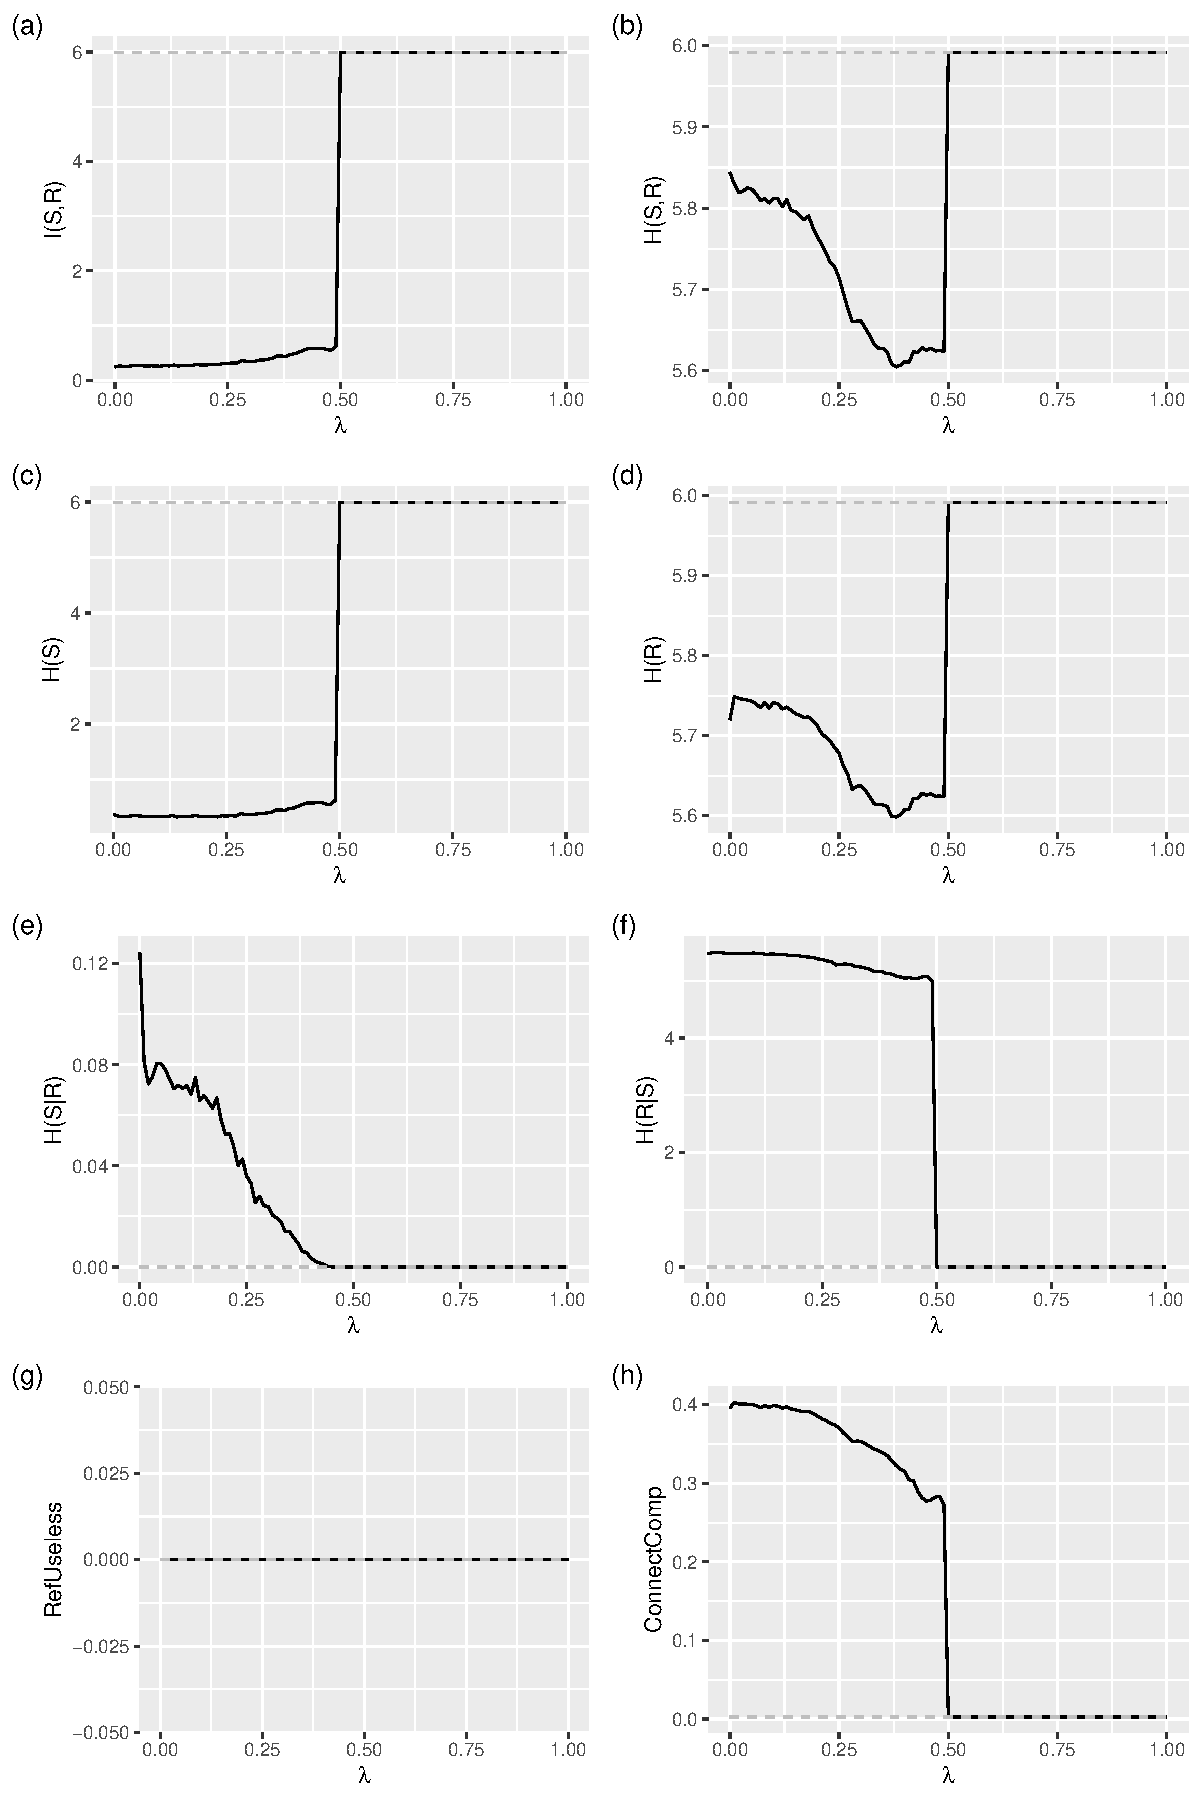
\includegraphics[width=\textwidth]{informationTheoretic_firstModel_phi0_nm400_dynamic_oneToOne_allowUnlinked}
  \caption{a}
  \label{fig:informationTheoretic_firstModel_phi0_nm400_dynamic_oneToOne_allowUnlinked}
\end{figure}

\begin{itemize}
\item initial: random \ref{fig:informationTheoretic_firstModel_phi0_nm400_dynamic_randomBipartite_allowUnlinked}
\item initial: single \ref{fig:informationTheoretic_firstModel_phi0_nm400_dynamic_singleLink_allowUnlinked}
\item initial: one-to-one \ref{fig:informationTheoretic_firstModel_phi0_nm400_dynamic_oneToOne_allowUnlinked}
\end{itemize}

\subsubsection{first model, $\phi=1$}

\begin{figure}
  \centering
  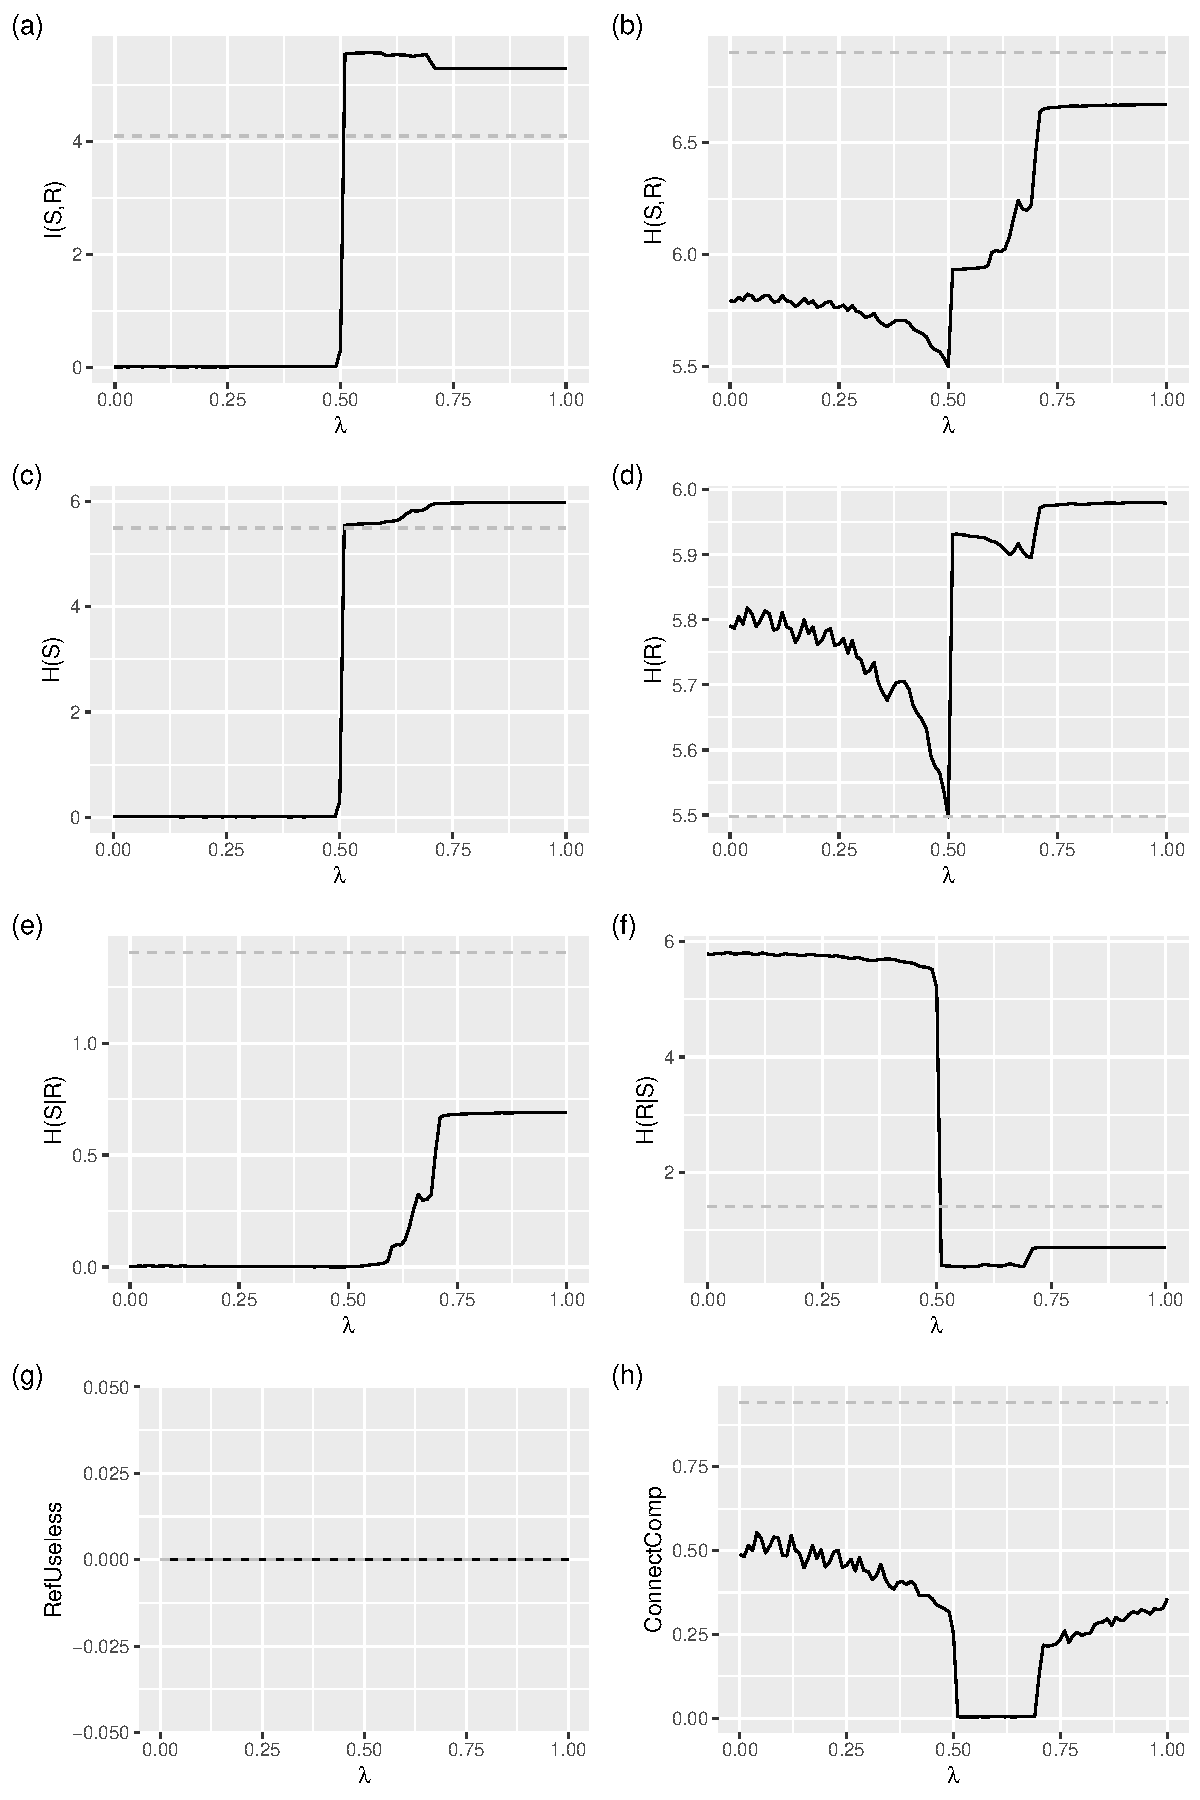
\includegraphics[width=\textwidth]{informationTheoretic_firstModel_phi1_nm400_dynamic_randomBipartite_allowUnlinked}
  \caption{a}
  \label{fig:informationTheoretic_firstModel_phi1_nm400_dynamic_randomBipartite_allowUnlinked}
\end{figure}

\begin{figure}
  \centering
  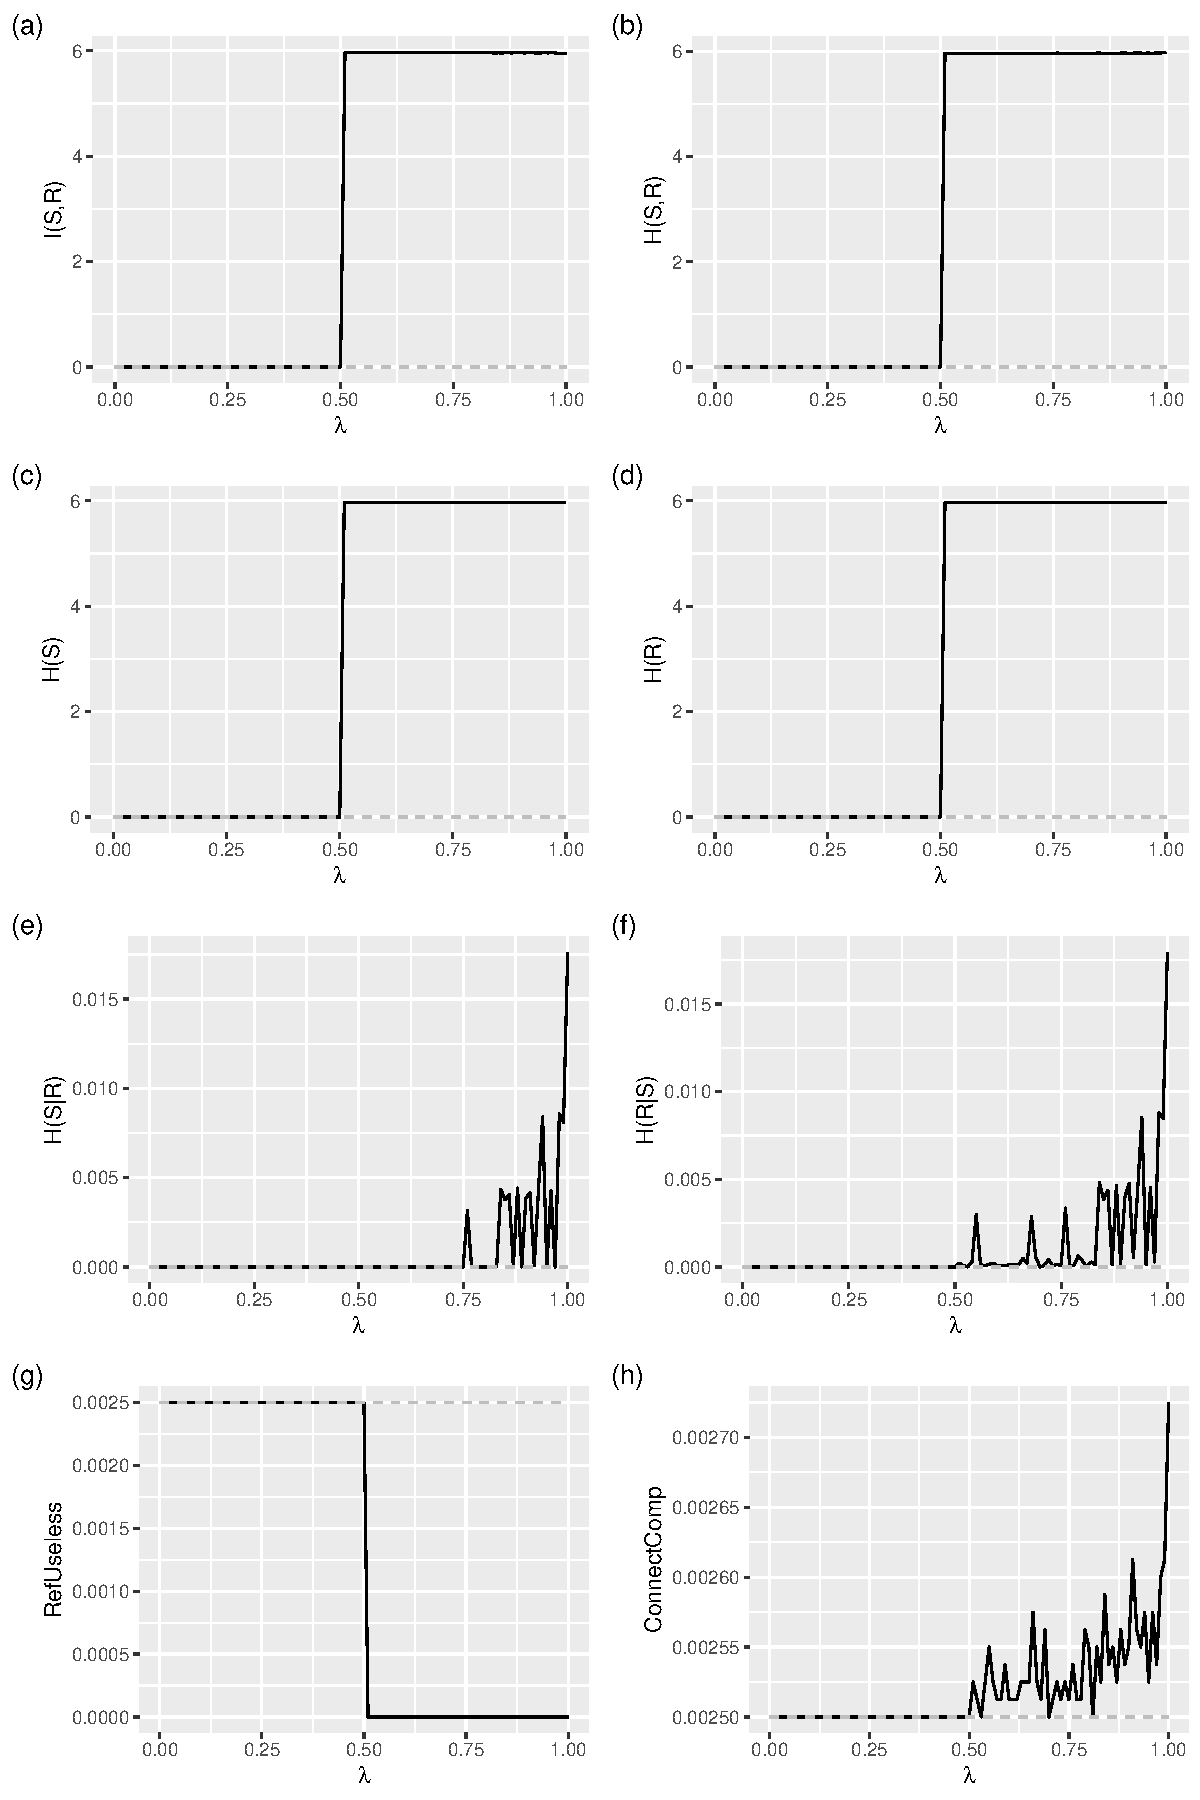
\includegraphics[width=\textwidth]{informationTheoretic_firstModel_phi1_nm400_dynamic_singleLink_allowUnlinked}
  \caption{a}
  \label{fig:informationTheoretic_firstModel_phi1_nm400_dynamic_singleLink_allowUnlinked}
\end{figure}

\begin{figure}
  \centering
  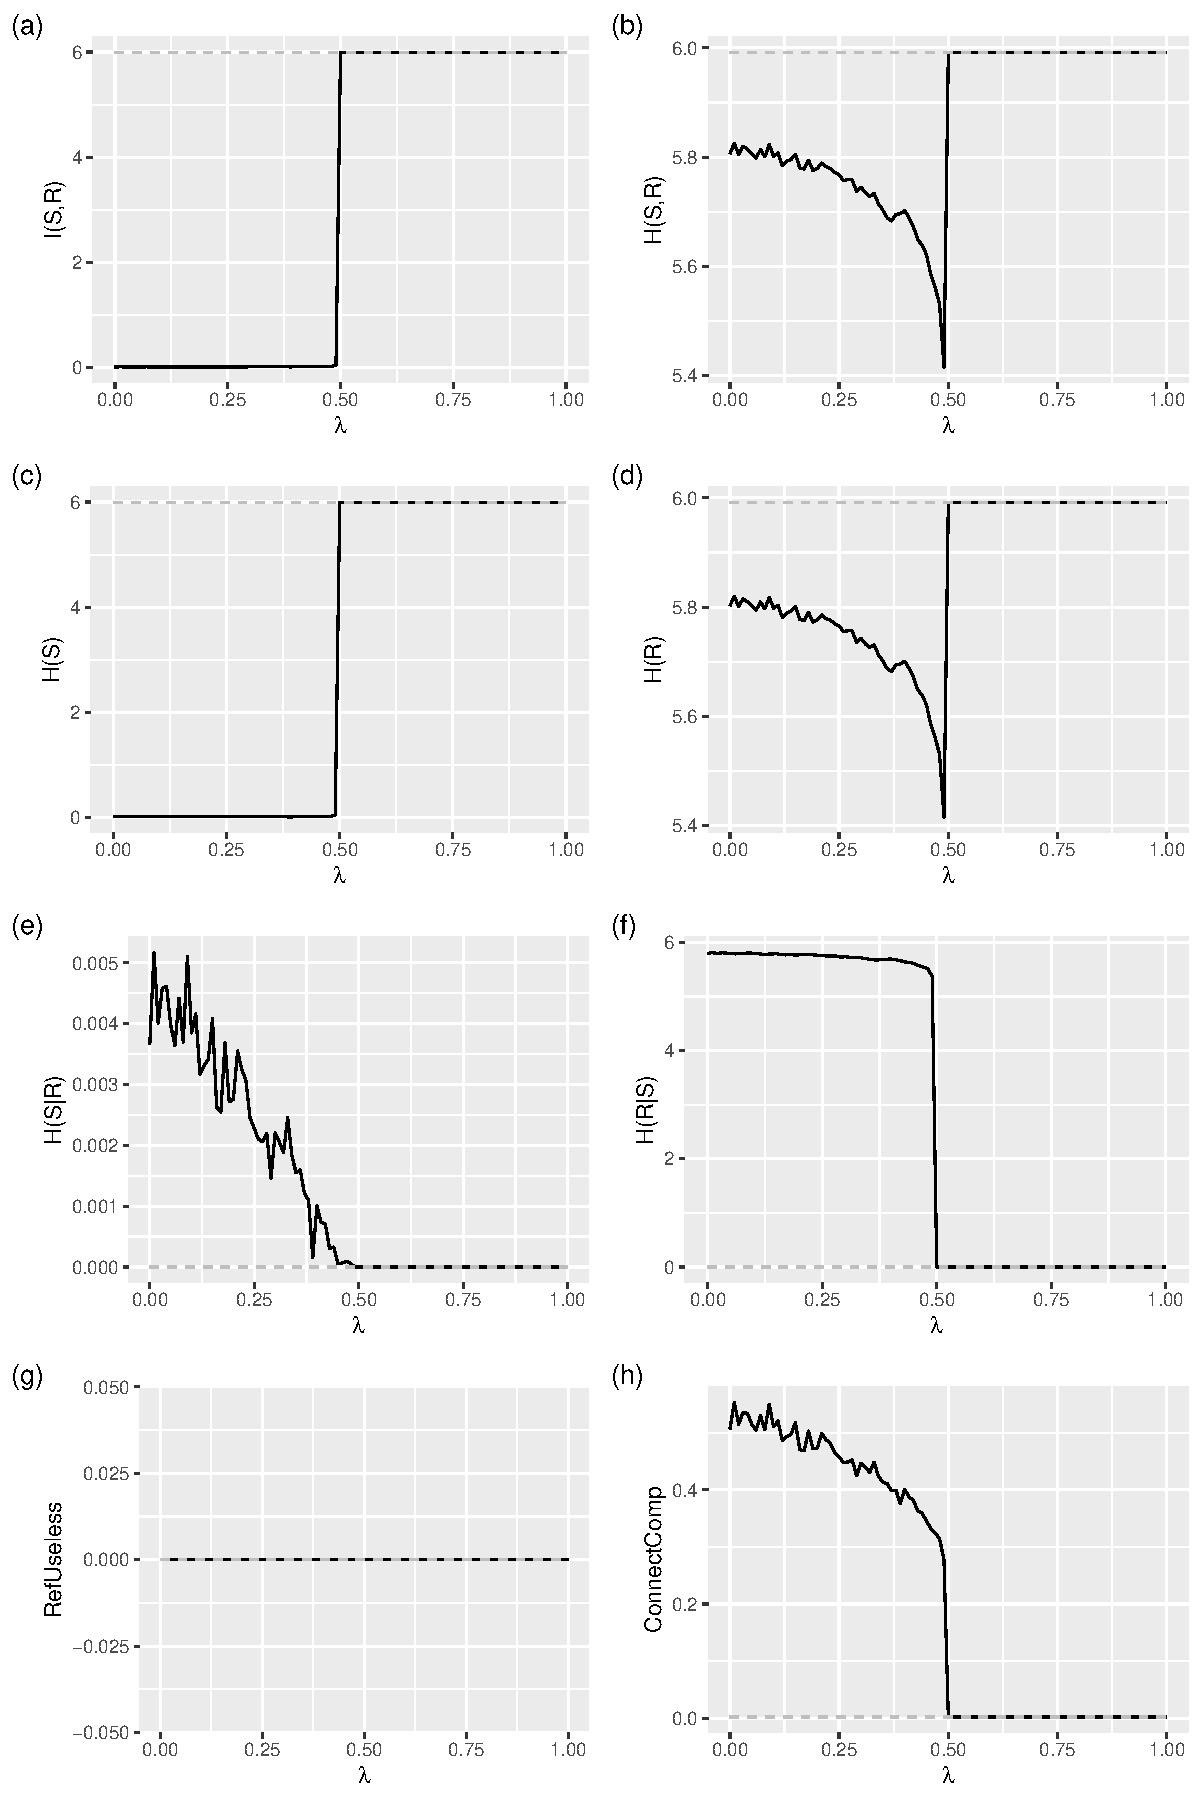
\includegraphics[width=\textwidth]{informationTheoretic_firstModel_phi1_nm400_dynamic_oneToOne_allowUnlinked}
  \caption{a}
  \label{fig:informationTheoretic_firstModel_phi1_nm400_dynamic_oneToOne_allowUnlinked}
\end{figure}

\begin{itemize}
\item initial: random \ref{fig:informationTheoretic_firstModel_phi1_nm400_dynamic_randomBipartite_allowUnlinked}
\item initial: single \ref{fig:informationTheoretic_firstModel_phi1_nm400_dynamic_singleLink_allowUnlinked}
\item initial: one-to-one \ref{fig:informationTheoretic_firstModel_phi1_nm400_dynamic_oneToOne_allowUnlinked}
\end{itemize}

\subsubsection{second model, $\phi=0$}

\begin{figure}
  \centering
  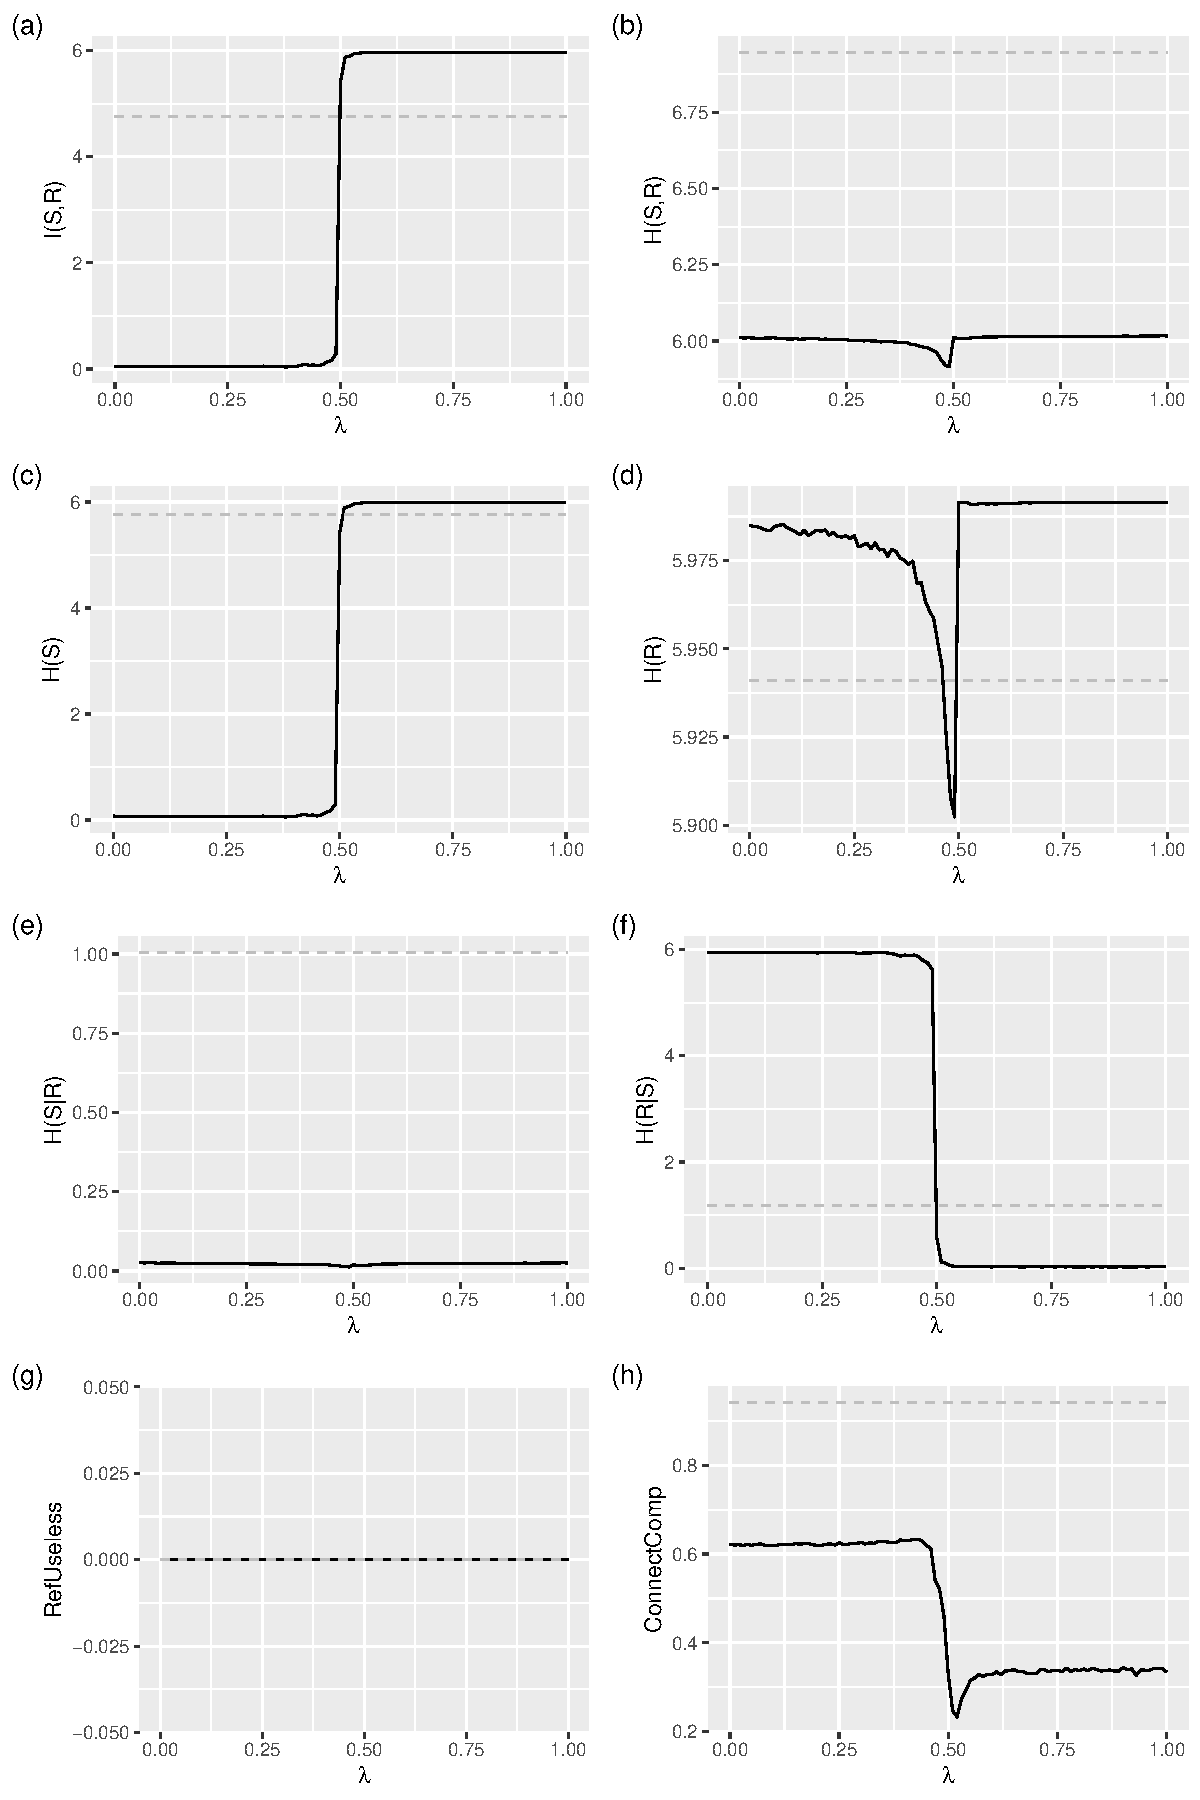
\includegraphics[width=\textwidth]{informationTheoretic_uniform_phi0_nm400_dynamic_randomBipartite_allowUnlinked}
  \caption{a}
  \label{fig:informationTheoretic_uniform_phi0_nm400_dynamic_randomBipartite_allowUnlinked}
\end{figure}

\begin{figure}
  \centering
  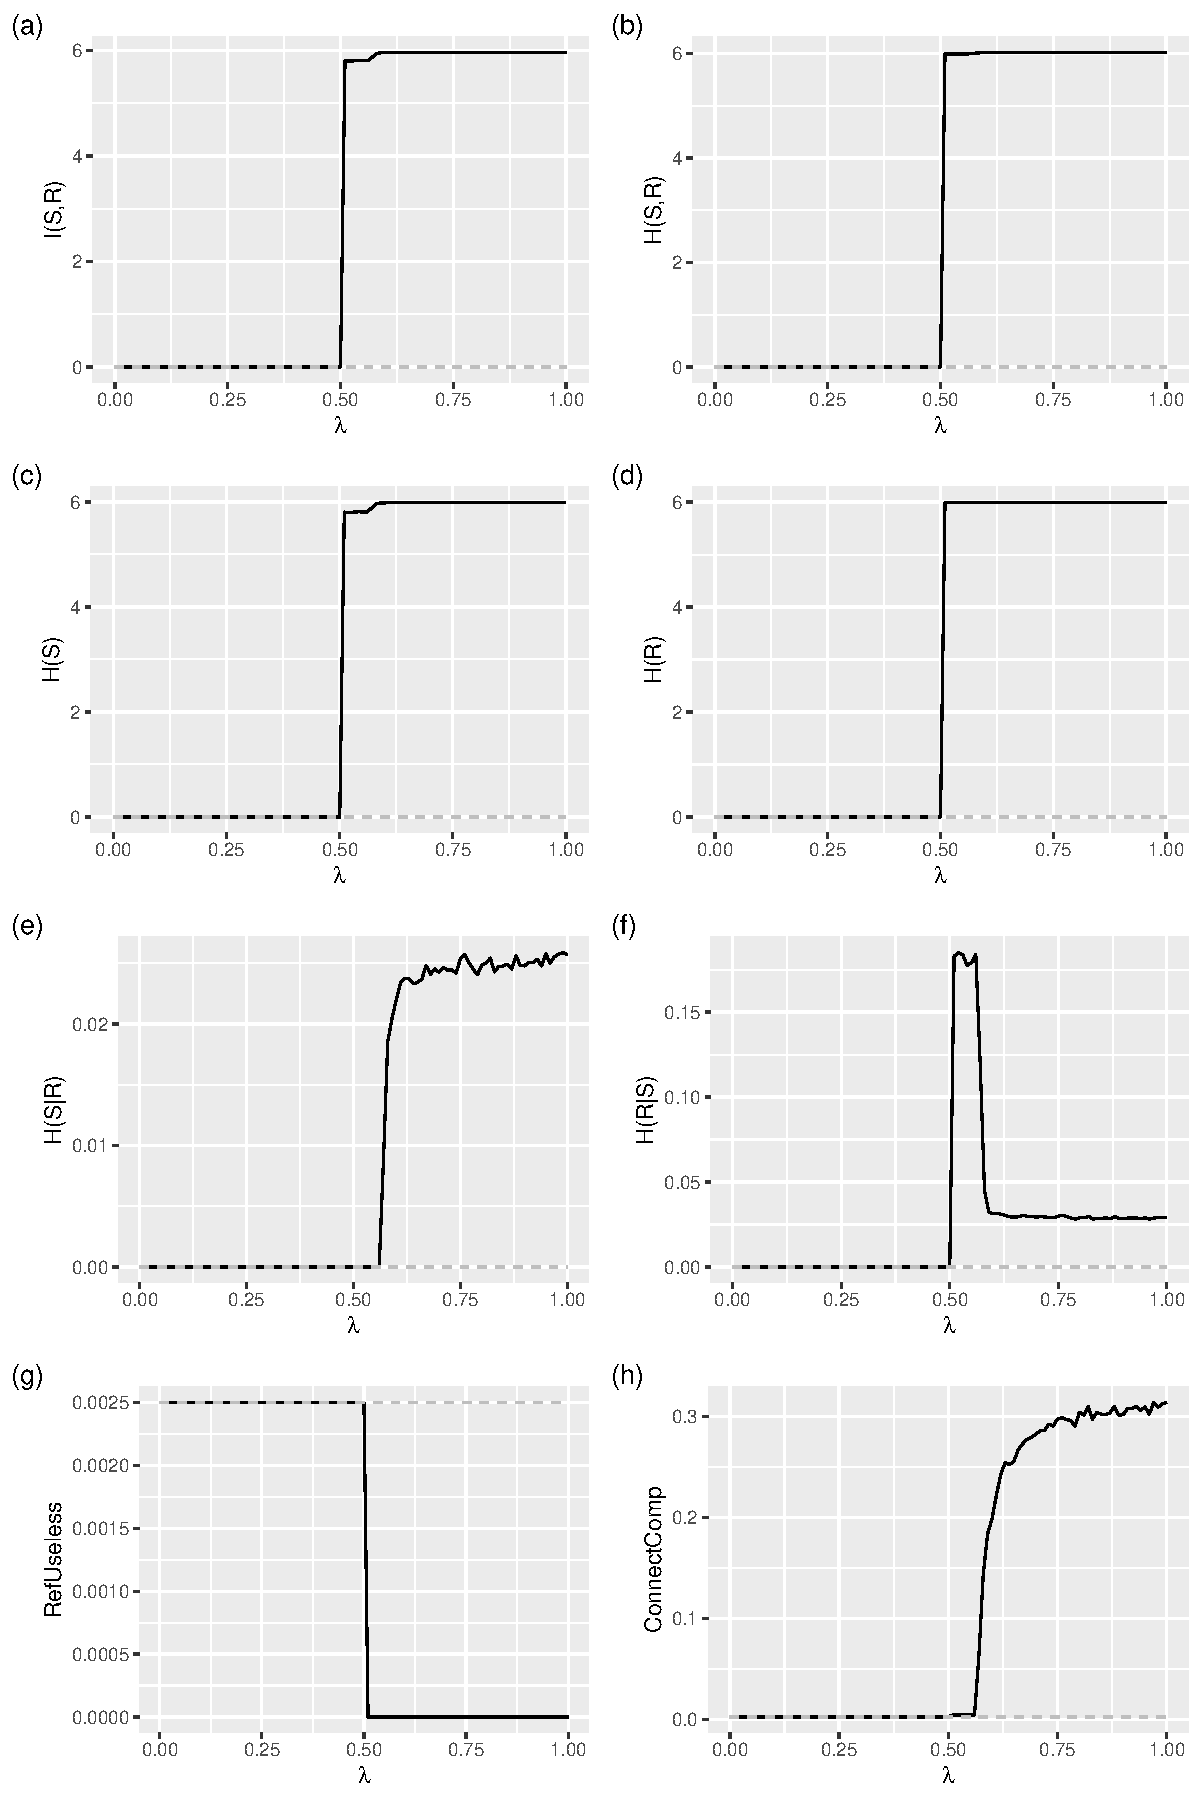
\includegraphics[width=\textwidth]{informationTheoretic_uniform_phi0_nm400_dynamic_singleLink_allowUnlinked}
  \caption{a}
  \label{fig:informationTheoretic_uniform_phi0_nm400_dynamic_singleLink_allowUnlinked}
\end{figure}

\begin{figure}
  \centering
  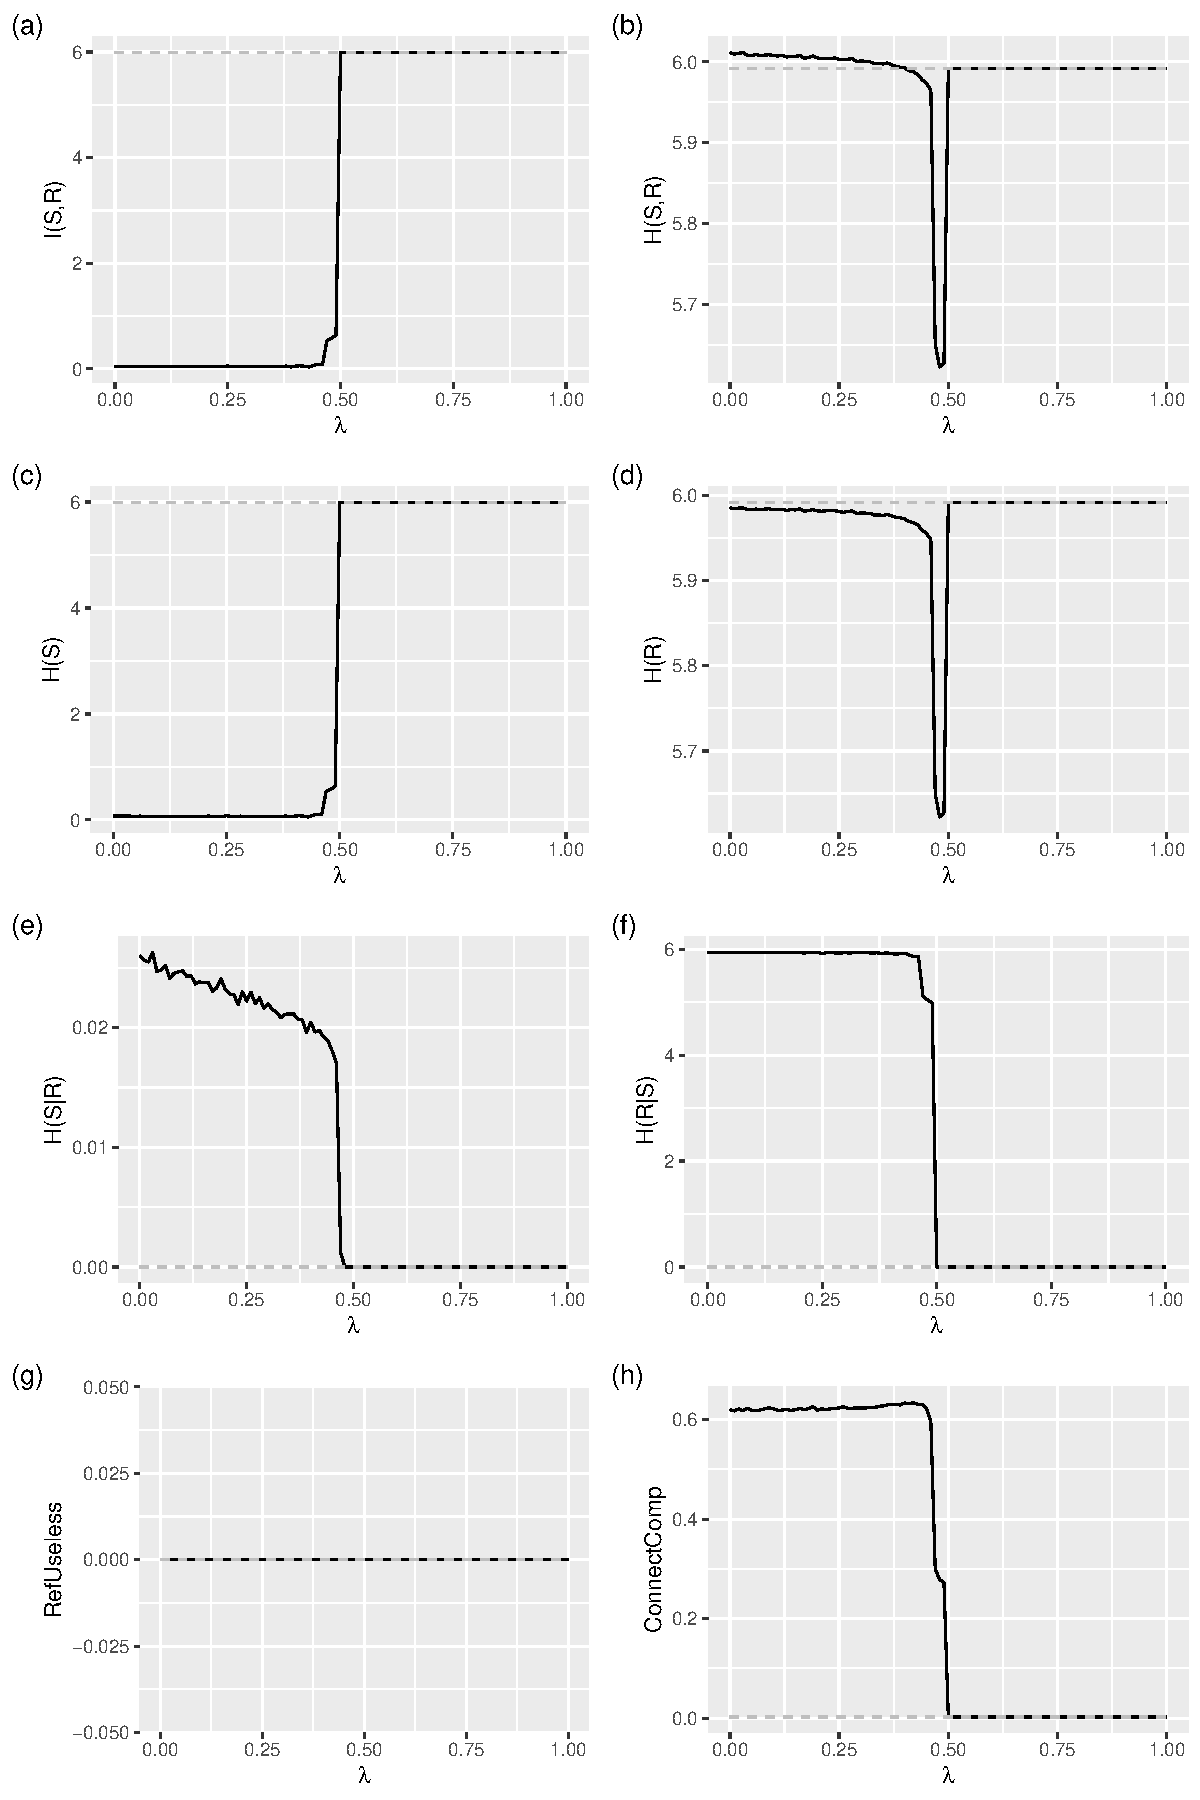
\includegraphics[width=\textwidth]{informationTheoretic_uniform_phi0_nm400_dynamic_oneToOne_allowUnlinked}
  \caption{a}
  \label{fig:informationTheoretic_uniform_phi0_nm400_dynamic_oneToOne_allowUnlinked}
\end{figure}

\begin{figure}
  \centering
  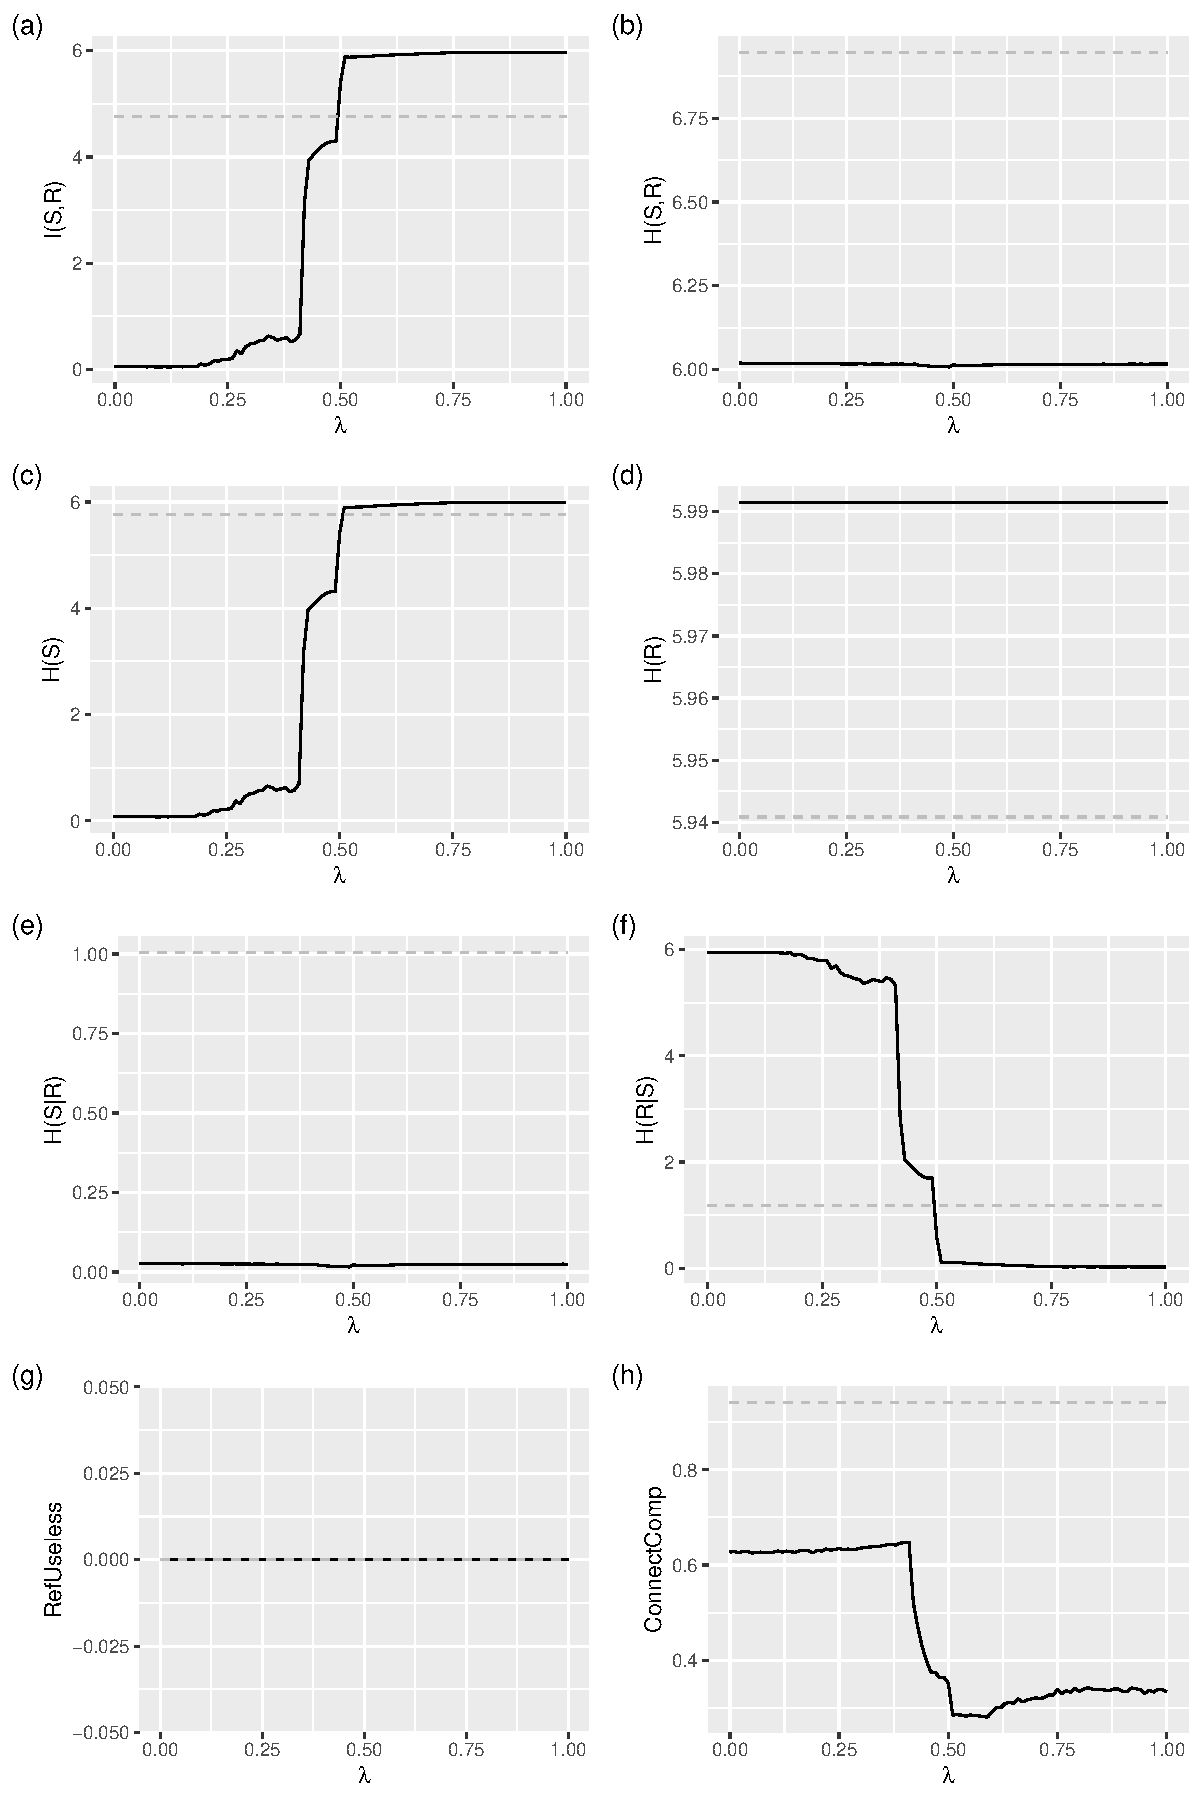
\includegraphics[width=\textwidth]{informationTheoretic_uniform_phi0_nm400_dynamic_randomBipartite_disallowUnlinked}
  \caption{a}
  \label{fig:informationTheoretic_uniform_phi0_nm400_dynamic_randomBipartite_disallowUnlinked}
\end{figure}

\begin{figure}
  \centering
  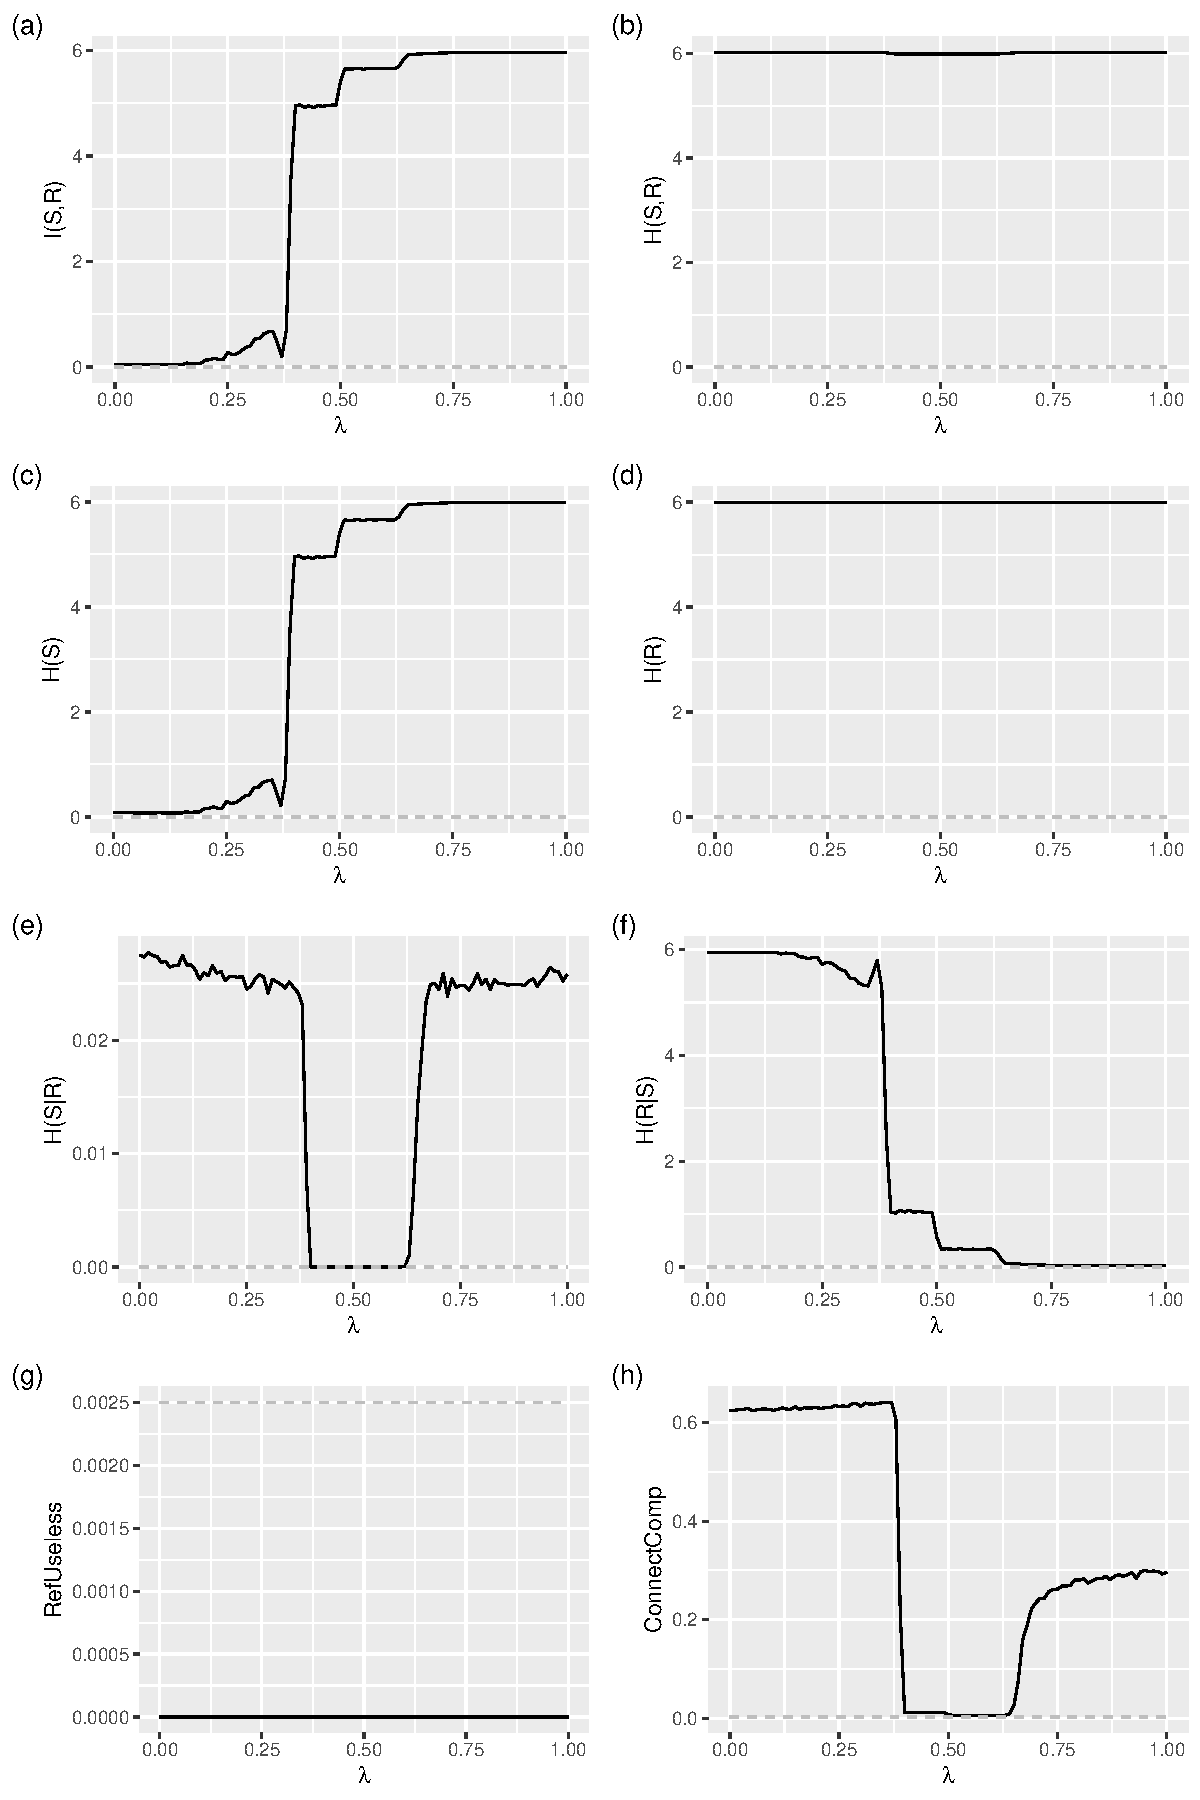
\includegraphics[width=\textwidth]{informationTheoretic_uniform_phi0_nm400_dynamic_singleLink_disallowUnlinked}
  \caption{a}
  \label{fig:informationTheoretic_uniform_phi0_nm400_dynamic_singleLink_disallowUnlinked}
\end{figure}

\begin{figure}
  \centering
  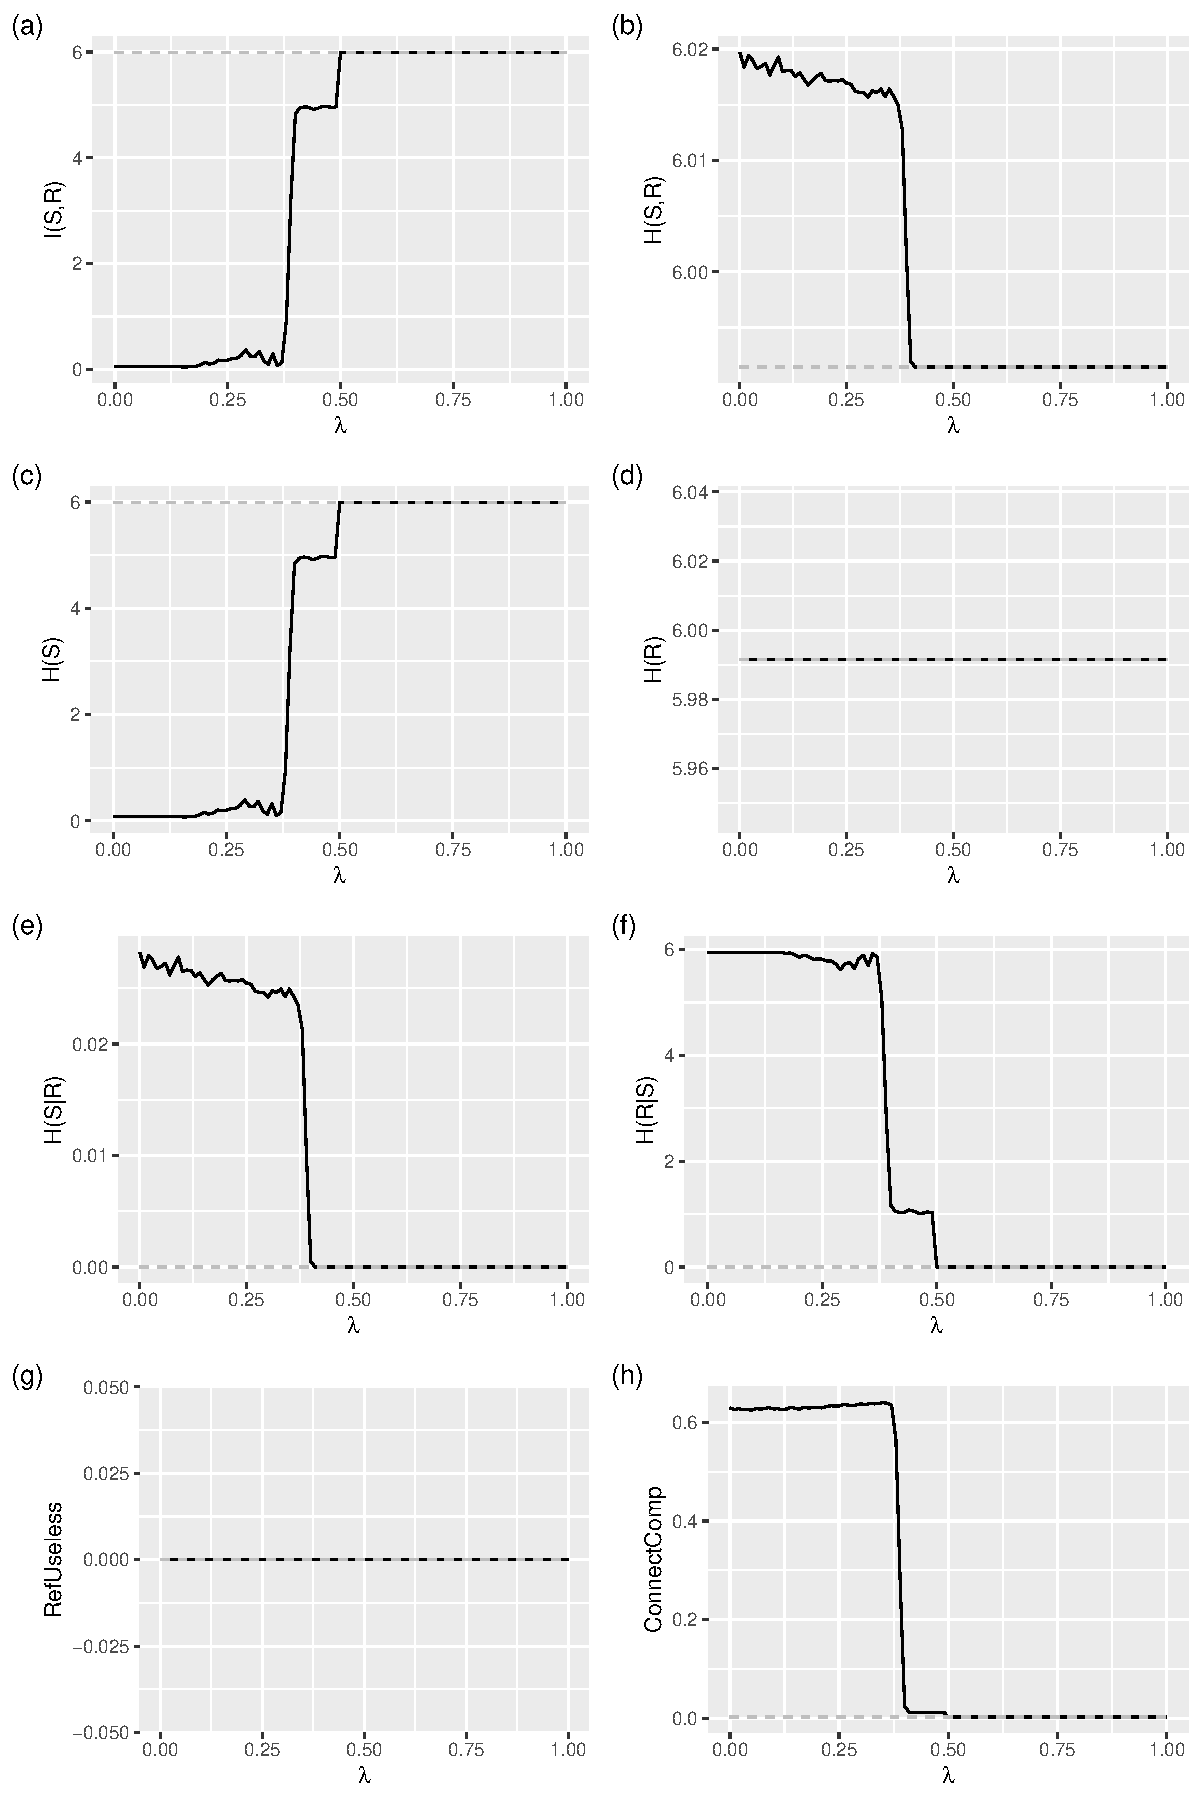
\includegraphics[width=\textwidth]{informationTheoretic_uniform_phi0_nm400_dynamic_oneToOne_disallowUnlinked}
  \caption{a}
  \label{fig:informationTheoretic_uniform_phi0_nm400_dynamic_oneToOne_disallowUnlinked}
\end{figure}

all $\pi$ uniform

\begin{itemize}
\item allow disconnect meanings
  \begin{itemize}
  \item initial: random \ref{fig:informationTheoretic_uniform_phi0_nm400_dynamic_randomBipartite_allowUnlinked}
  \item initial: single \ref{fig:informationTheoretic_uniform_phi0_nm400_dynamic_singleLink_allowUnlinked}
  \item initial: one-to-one \ref{fig:informationTheoretic_uniform_phi0_nm400_dynamic_oneToOne_allowUnlinked}
  \end{itemize}
\item do not allow disconnect meanings
  \begin{itemize}
  \item initial: random \ref{fig:informationTheoretic_uniform_phi0_nm400_dynamic_randomBipartite_disallowUnlinked}
  \item initial: single \ref{fig:informationTheoretic_uniform_phi0_nm400_dynamic_singleLink_disallowUnlinked}
  \item initial: one-to-one \ref{fig:informationTheoretic_uniform_phi0_nm400_dynamic_oneToOne_disallowUnlinked}
  \end{itemize}
\end{itemize}

\subsubsection{second model, $\phi=1$}

\begin{figure}
  \centering
  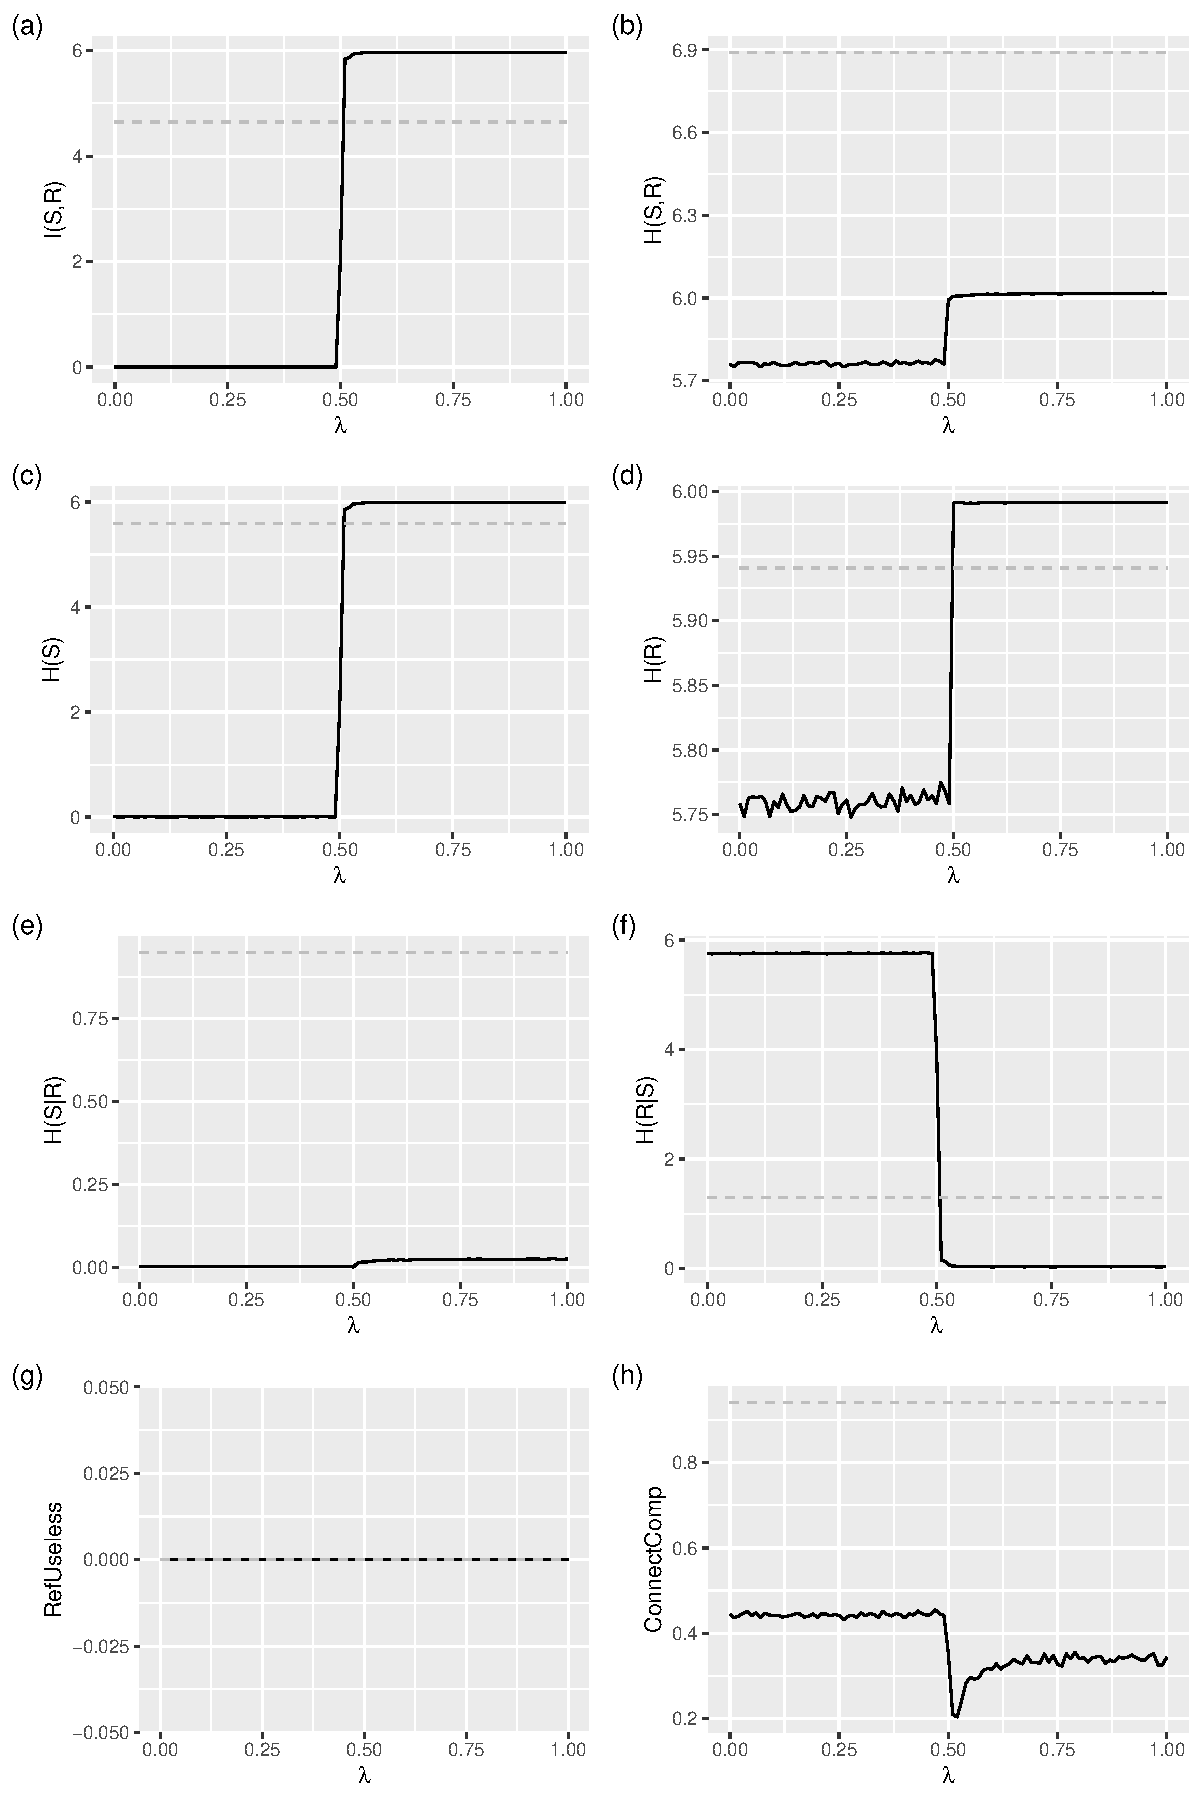
\includegraphics[width=\textwidth]{informationTheoretic_uniform_phi1_nm400_dynamic_randomBipartite_allowUnlinked}
  \caption{a}
  \label{fig:informationTheoretic_uniform_phi1_nm400_dynamic_randomBipartite_allowUnlinked}
\end{figure}

\begin{figure}
  \centering
  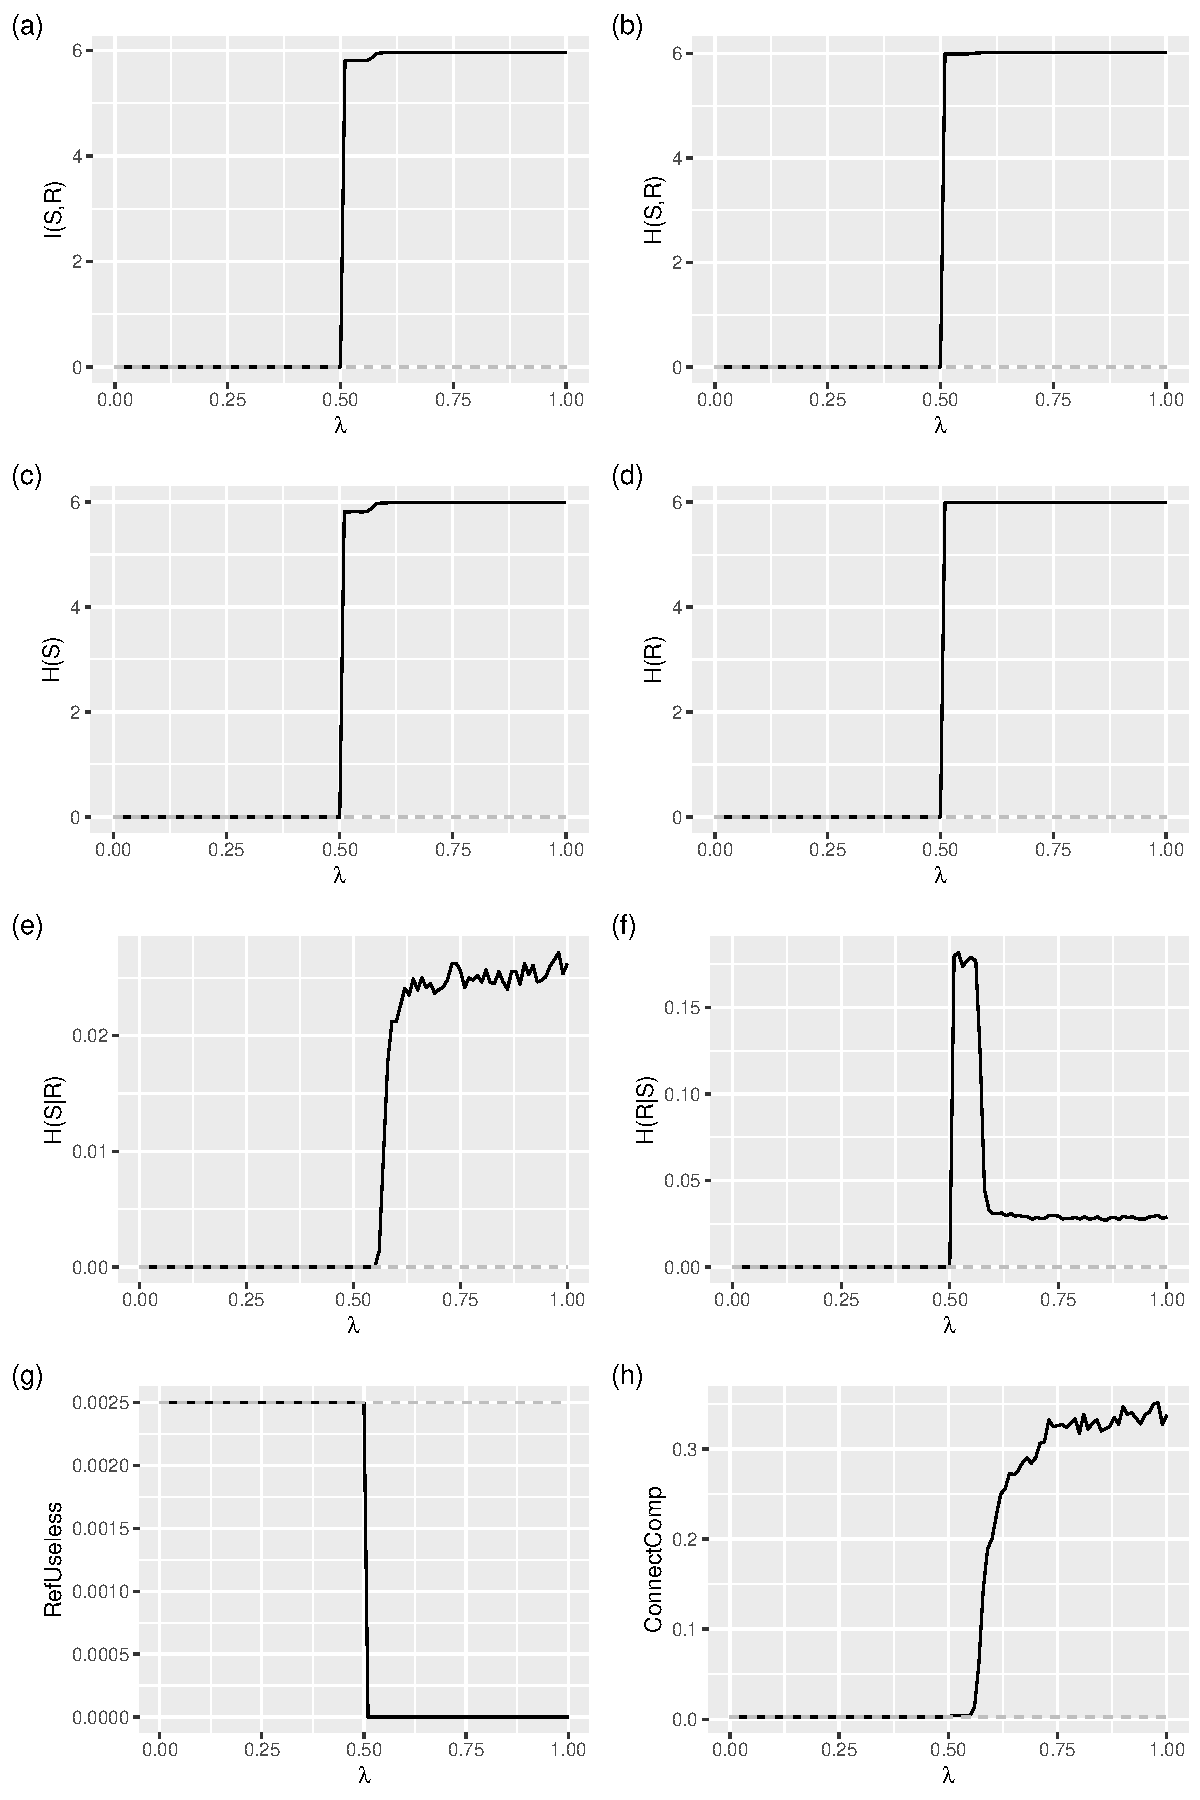
\includegraphics[width=\textwidth,draft]{informationTheoretic_uniform_phi1_nm400_dynamic_singleLink_allowUnlinked.pdf}
  \caption{a}
  \label{fig:informationTheoretic_uniform_phi1_nm400_dynamic_singleLink_allowUnlinked}
\end{figure}

\begin{figure}
  \centering
  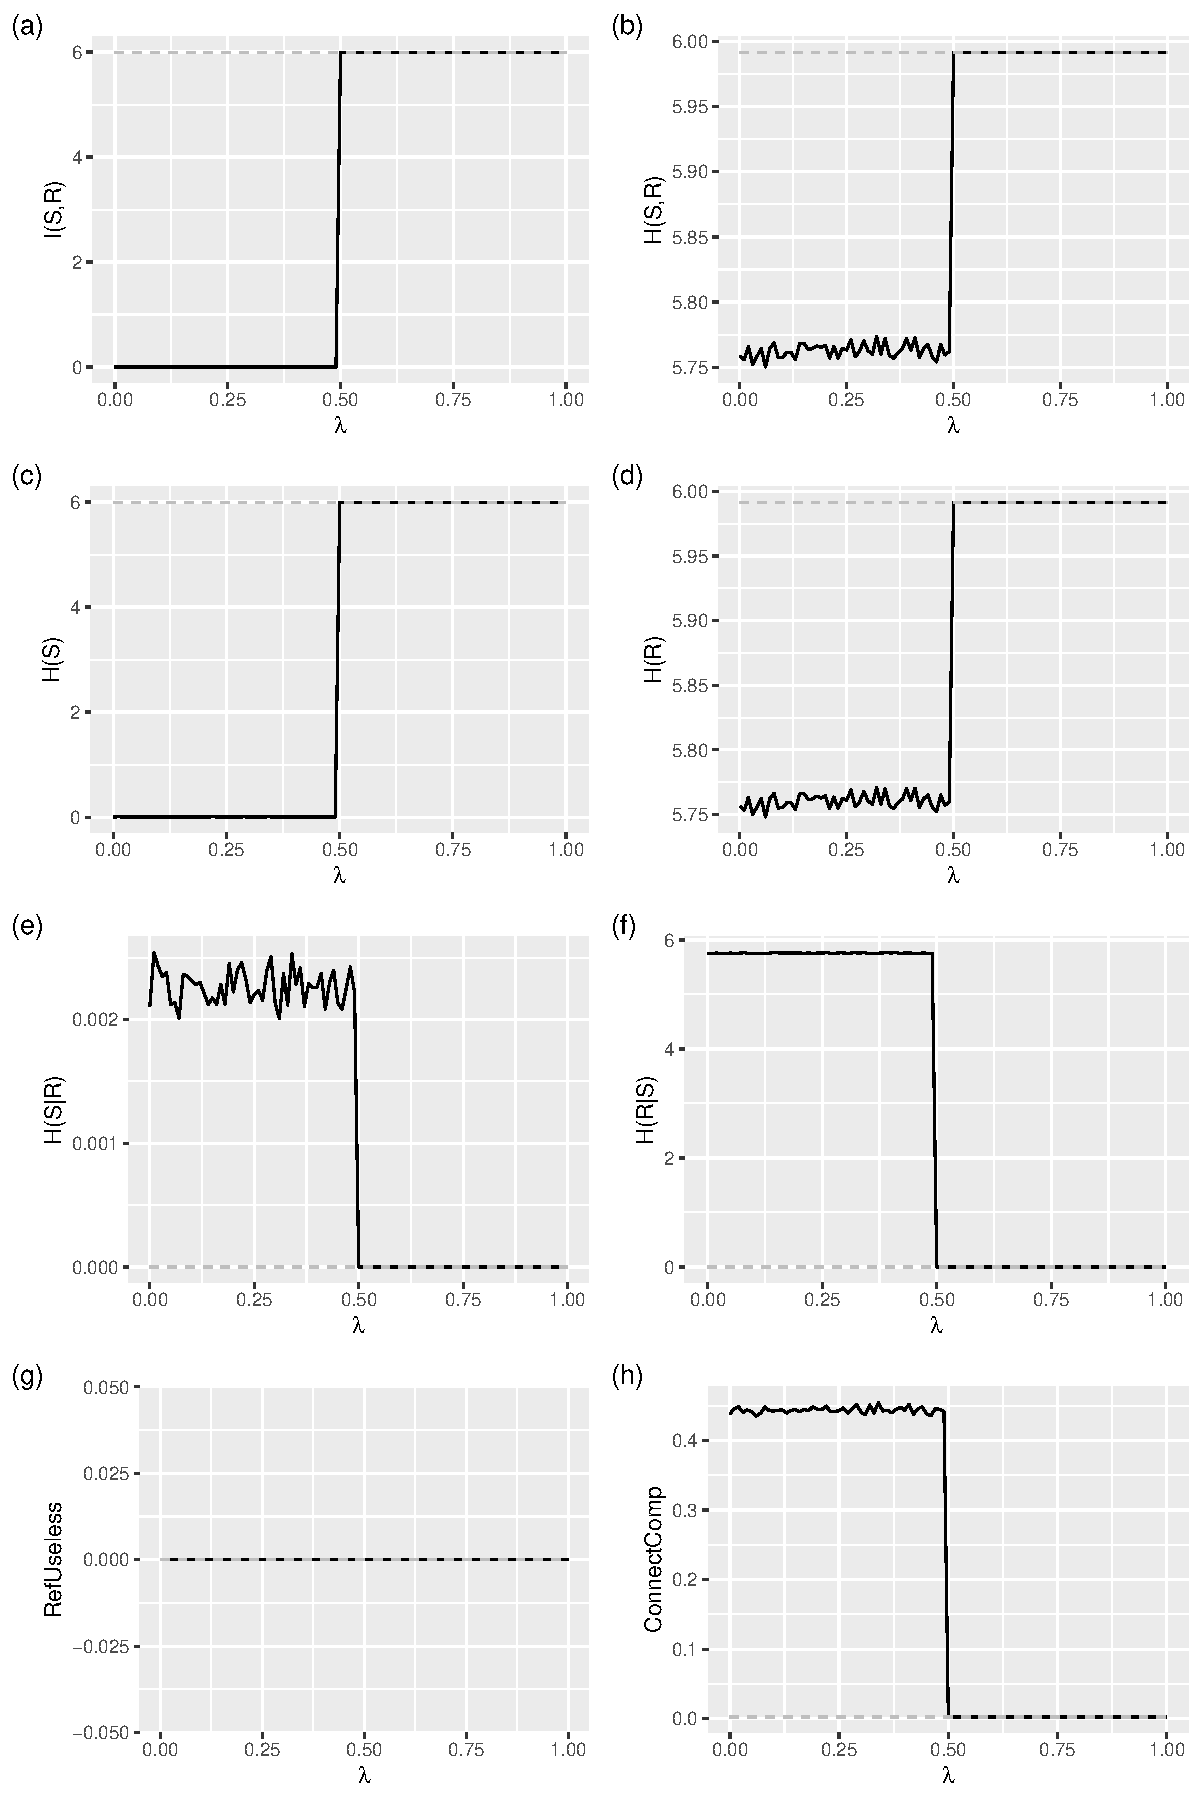
\includegraphics[width=\textwidth]{informationTheoretic_uniform_phi1_nm400_dynamic_oneToOne_allowUnlinked}
  \caption{a}
  \label{fig:informationTheoretic_uniform_phi1_nm400_dynamic_oneToOne_allowUnlinked}
\end{figure}

\begin{figure}
  \centering
  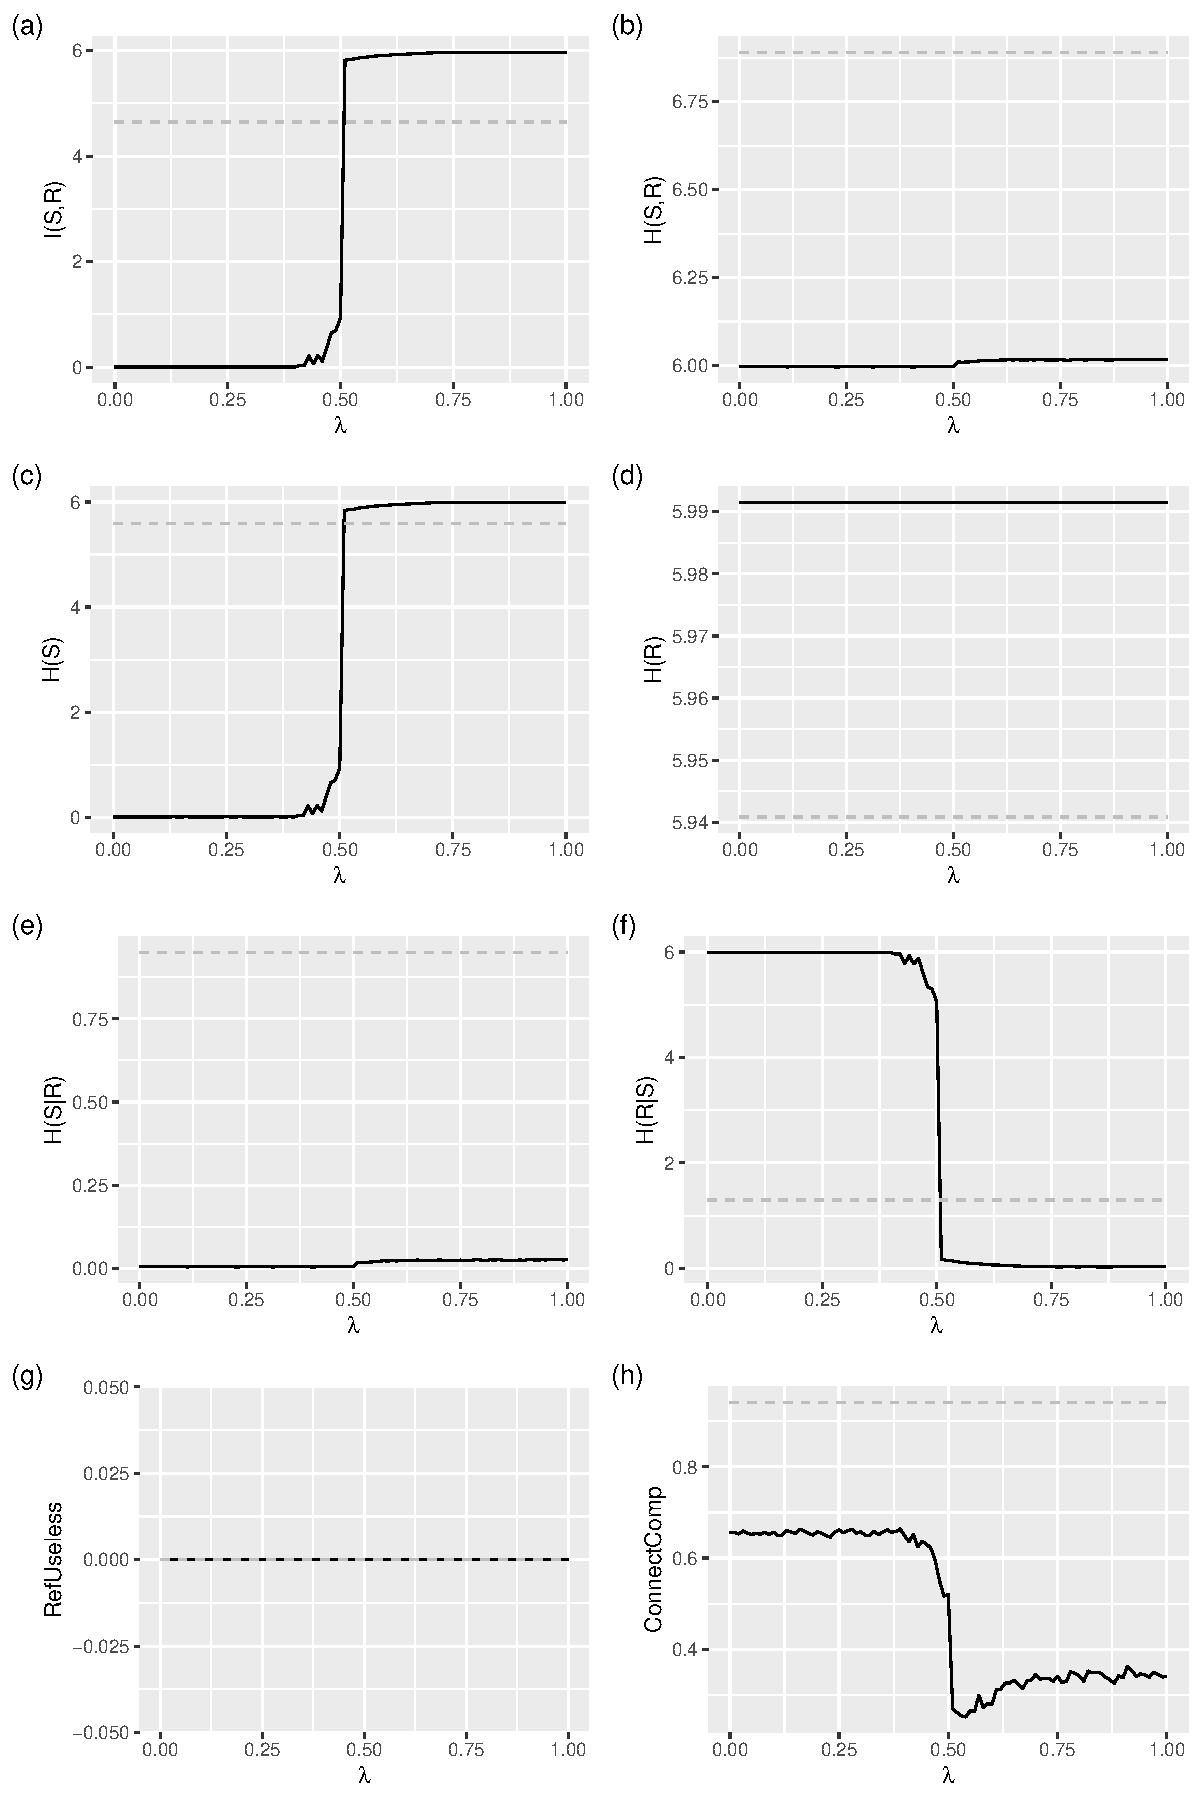
\includegraphics[width=\textwidth]{informationTheoretic_uniform_phi1_nm400_dynamic_randomBipartite_disallowUnlinked}
  \caption{a}
  \label{fig:informationTheoretic_uniform_phi1_nm400_dynamic_randomBipartite_disallowUnlinked}
\end{figure}

\begin{figure}
  \centering
  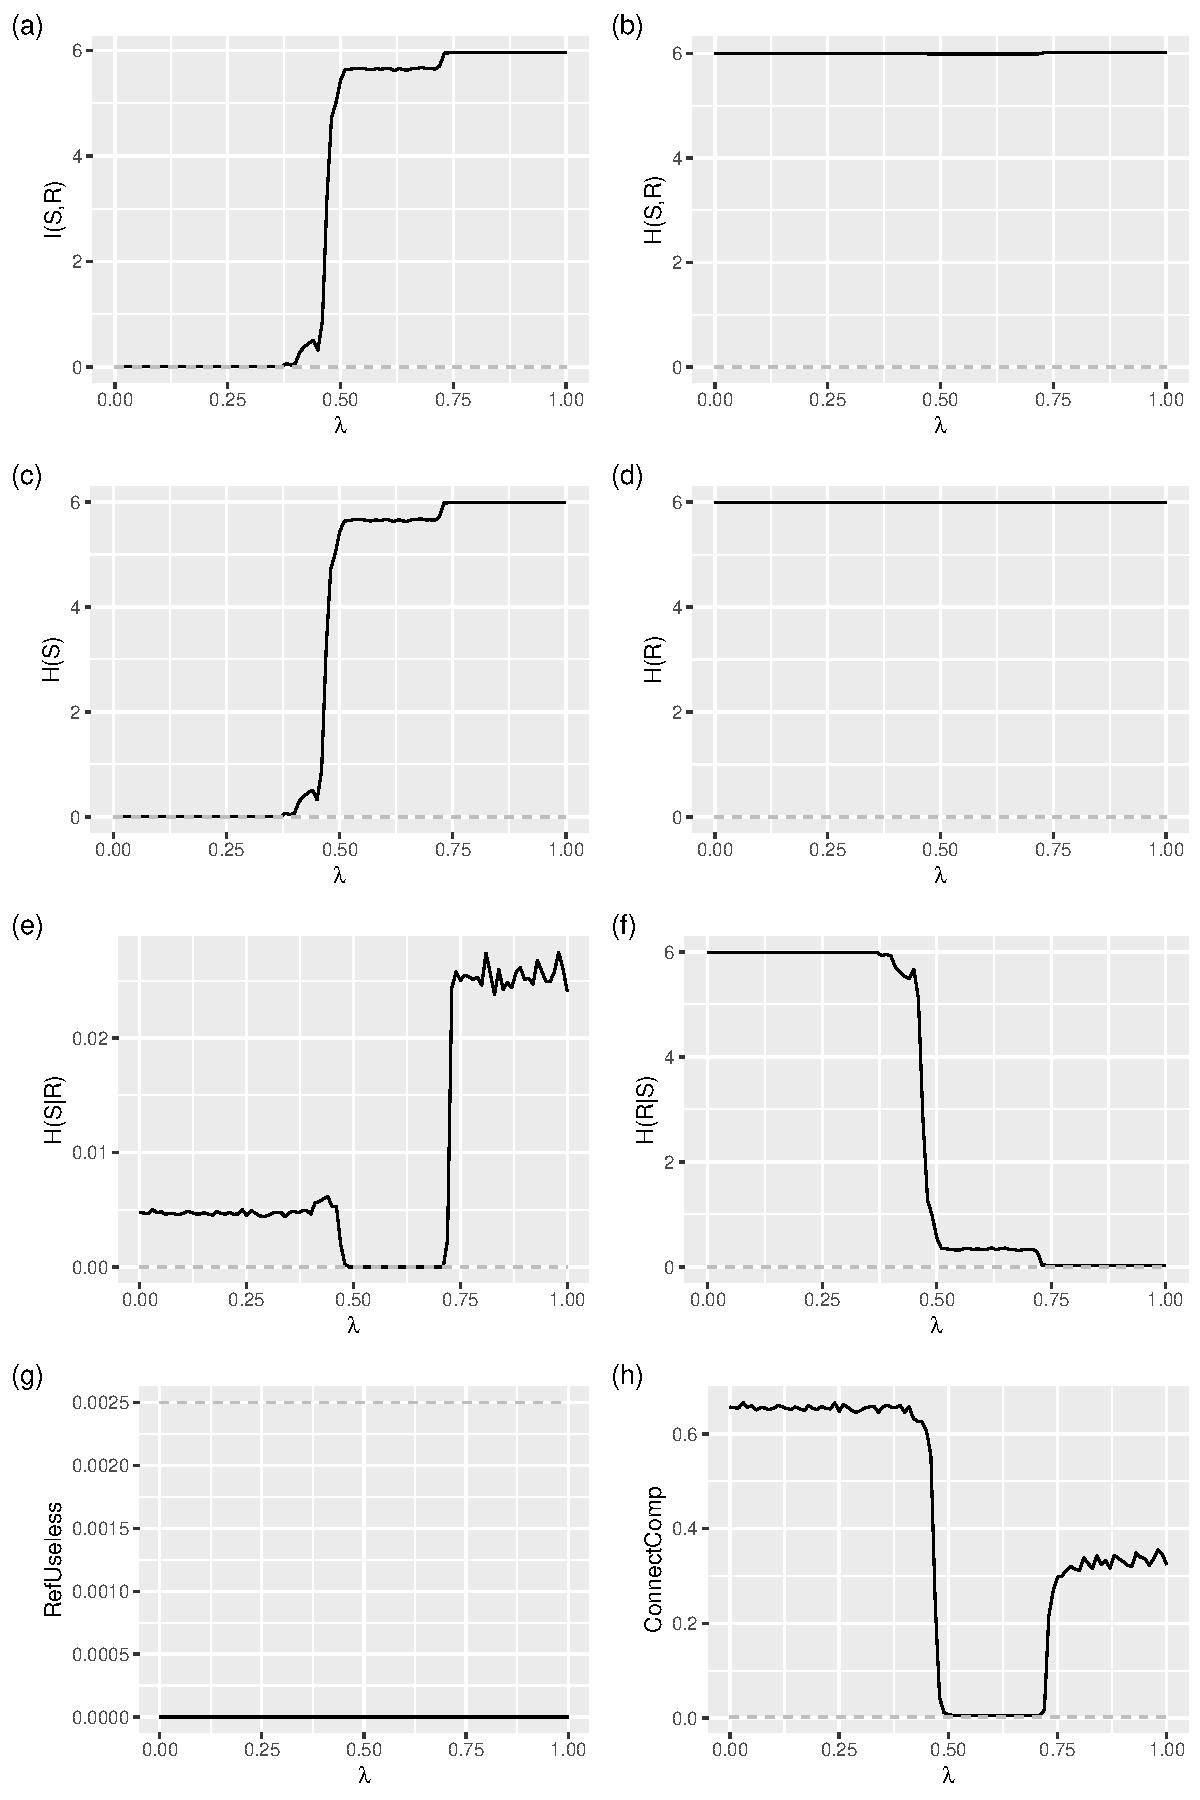
\includegraphics[width=\textwidth]{informationTheoretic_uniform_phi1_nm400_dynamic_singleLink_disallowUnlinked}
  \caption{a}
  \label{fig:informationTheoretic_uniform_phi1_nm400_dynamic_singleLink_disallowUnlinked}
\end{figure}

\begin{figure}
  \centering
  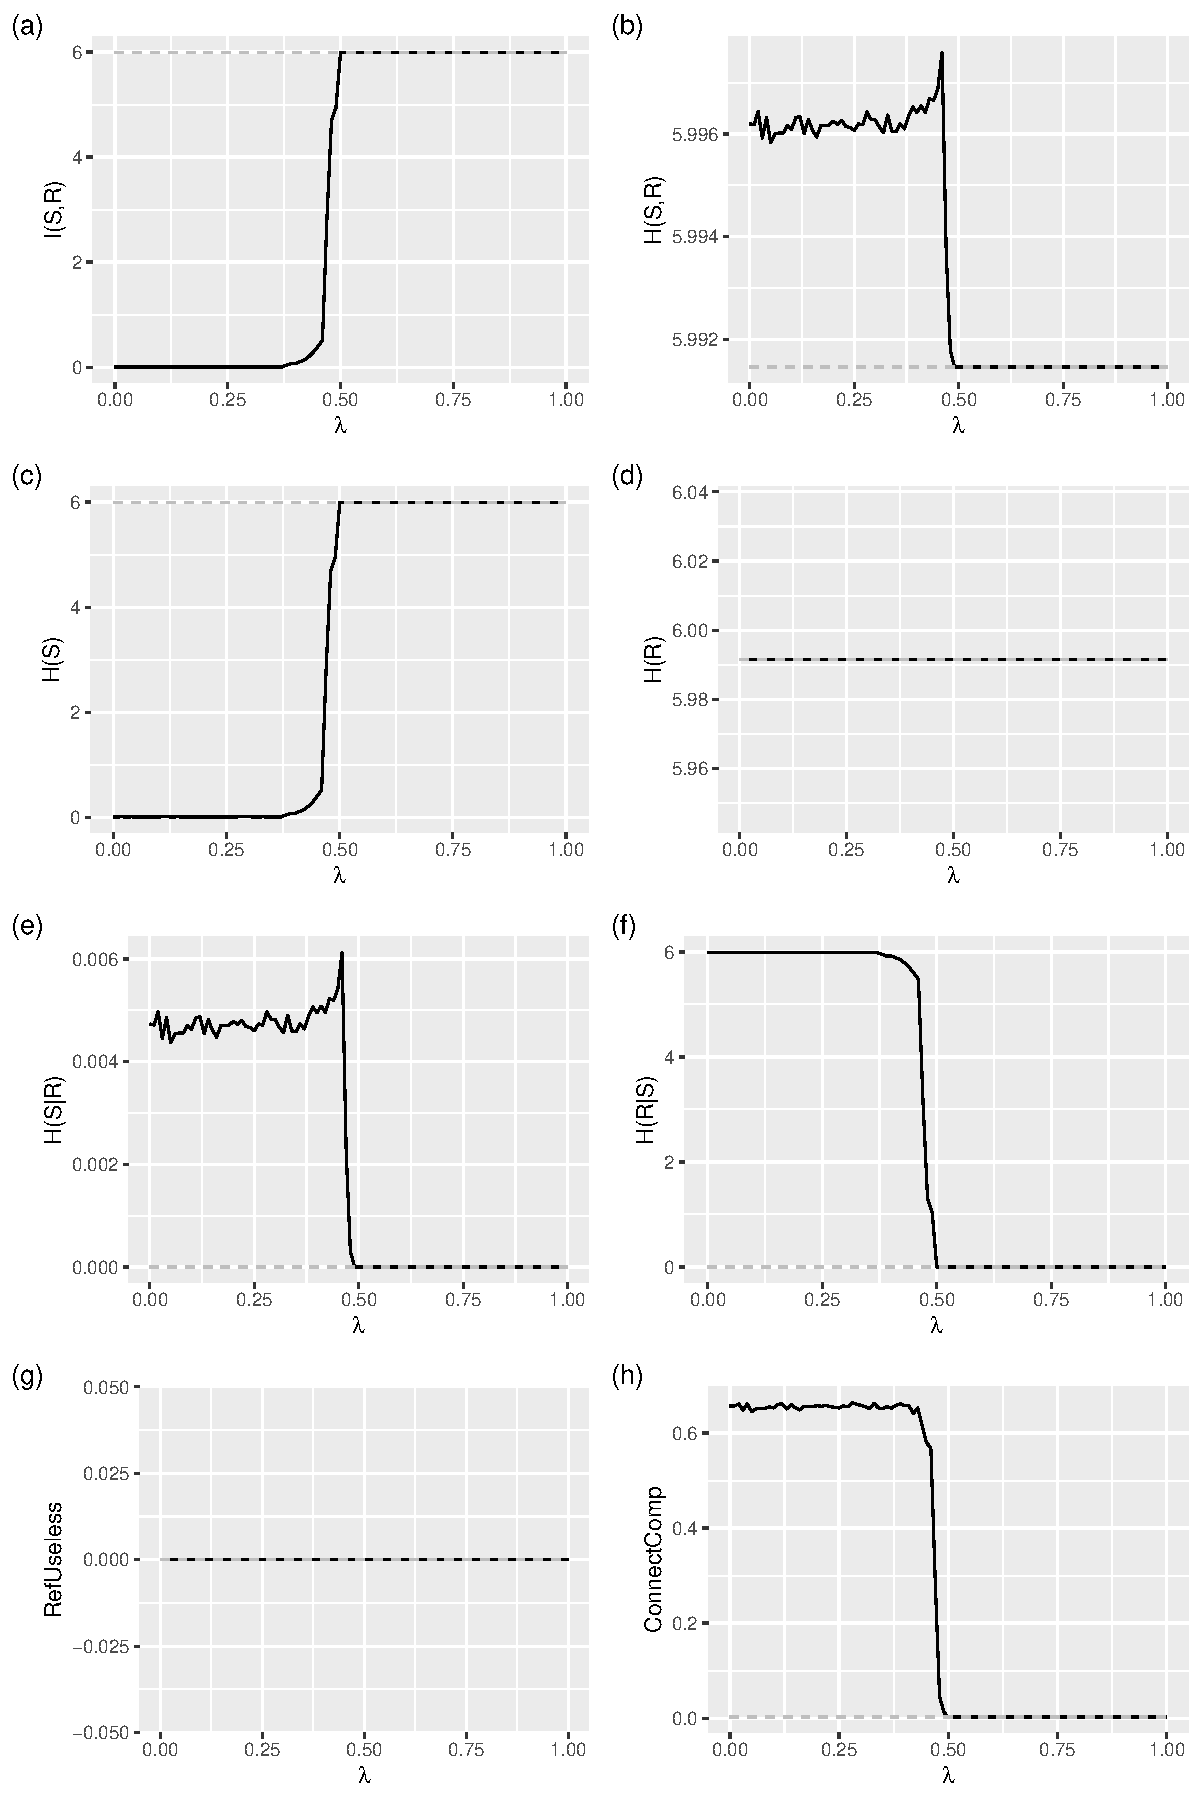
\includegraphics[width=\textwidth]{informationTheoretic_uniform_phi1_nm400_dynamic_oneToOne_disallowUnlinked}
  \caption{this happens for $\phi=1$ but not for $\phi=0$}
  \label{fig:informationTheoretic_uniform_phi1_nm400_dynamic_oneToOne_disallowUnlinked}
\end{figure}

all $\pi$ uniform

\begin{itemize}
\item allow disconnect meanings
  \begin{itemize}
  \item initial: random \ref{fig:informationTheoretic_uniform_phi1_nm400_dynamic_randomBipartite_allowUnlinked}
  \item initial: single \ref{fig:informationTheoretic_uniform_phi1_nm400_dynamic_singleLink_allowUnlinked}
  \item initial: one-to-one \ref{fig:informationTheoretic_uniform_phi1_nm400_dynamic_oneToOne_allowUnlinked}
  \end{itemize}
\item do not allow disconnect meanings
  \begin{itemize}
  \item initial: random \ref{fig:informationTheoretic_uniform_phi1_nm400_dynamic_randomBipartite_disallowUnlinked}
  \item initial: single \ref{fig:informationTheoretic_uniform_phi1_nm400_dynamic_singleLink_disallowUnlinked}
  \item initial: one-to-one \ref{fig:informationTheoretic_uniform_phi1_nm400_dynamic_oneToOne_disallowUnlinked}
  \end{itemize}
\end{itemize}

\subsection{Inside selected lambda}

\subsubsection{first model, $\phi=0$}

\begin{figure}
  \centering
  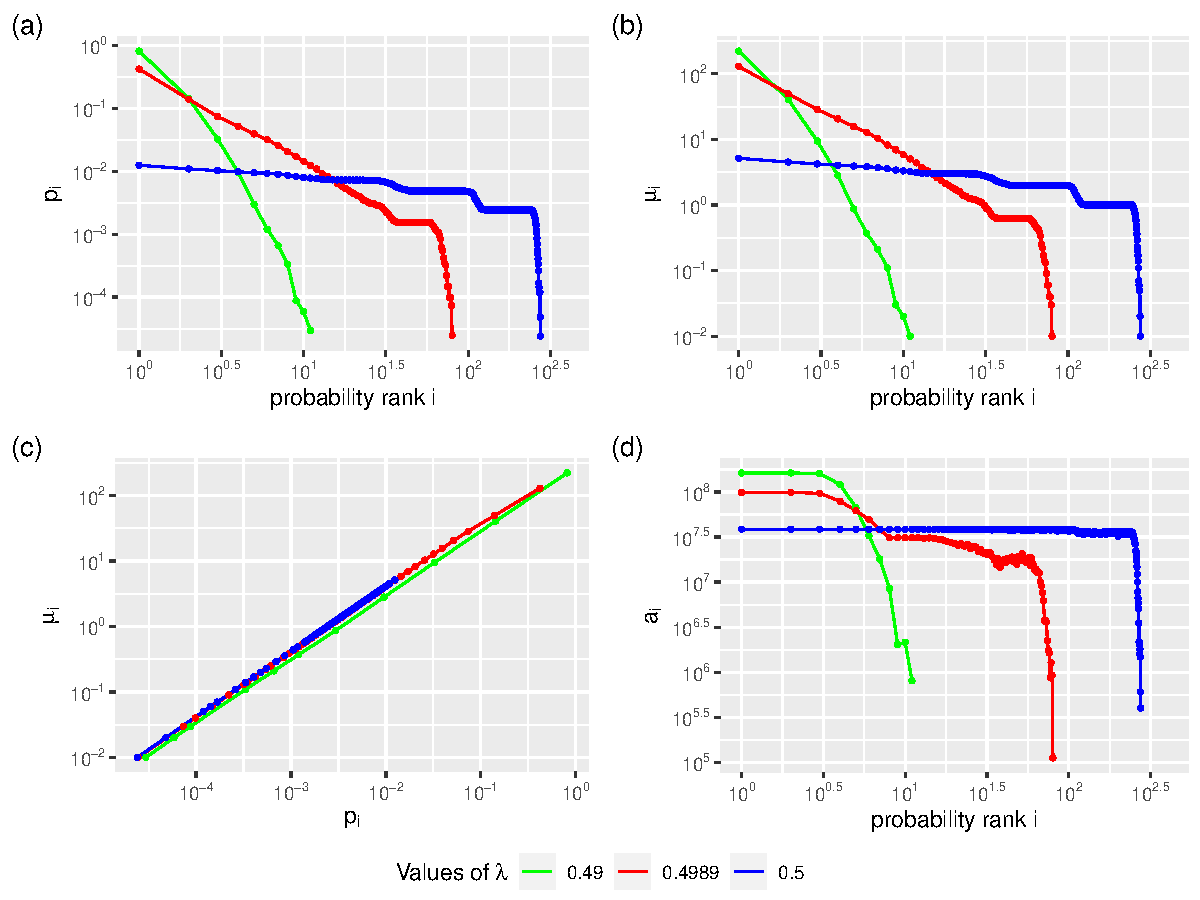
\includegraphics[width=\textwidth]{insideLambda_firstModel_phi0_nm400_dynamic_randomBipartite_allowUnlinked}
  \caption{a}
  \label{fig:insideLambda_firstModel_phi0_nm400_dynamic_randomBipartite_allowUnlinked}
\end{figure}

\begin{figure}
  \centering
  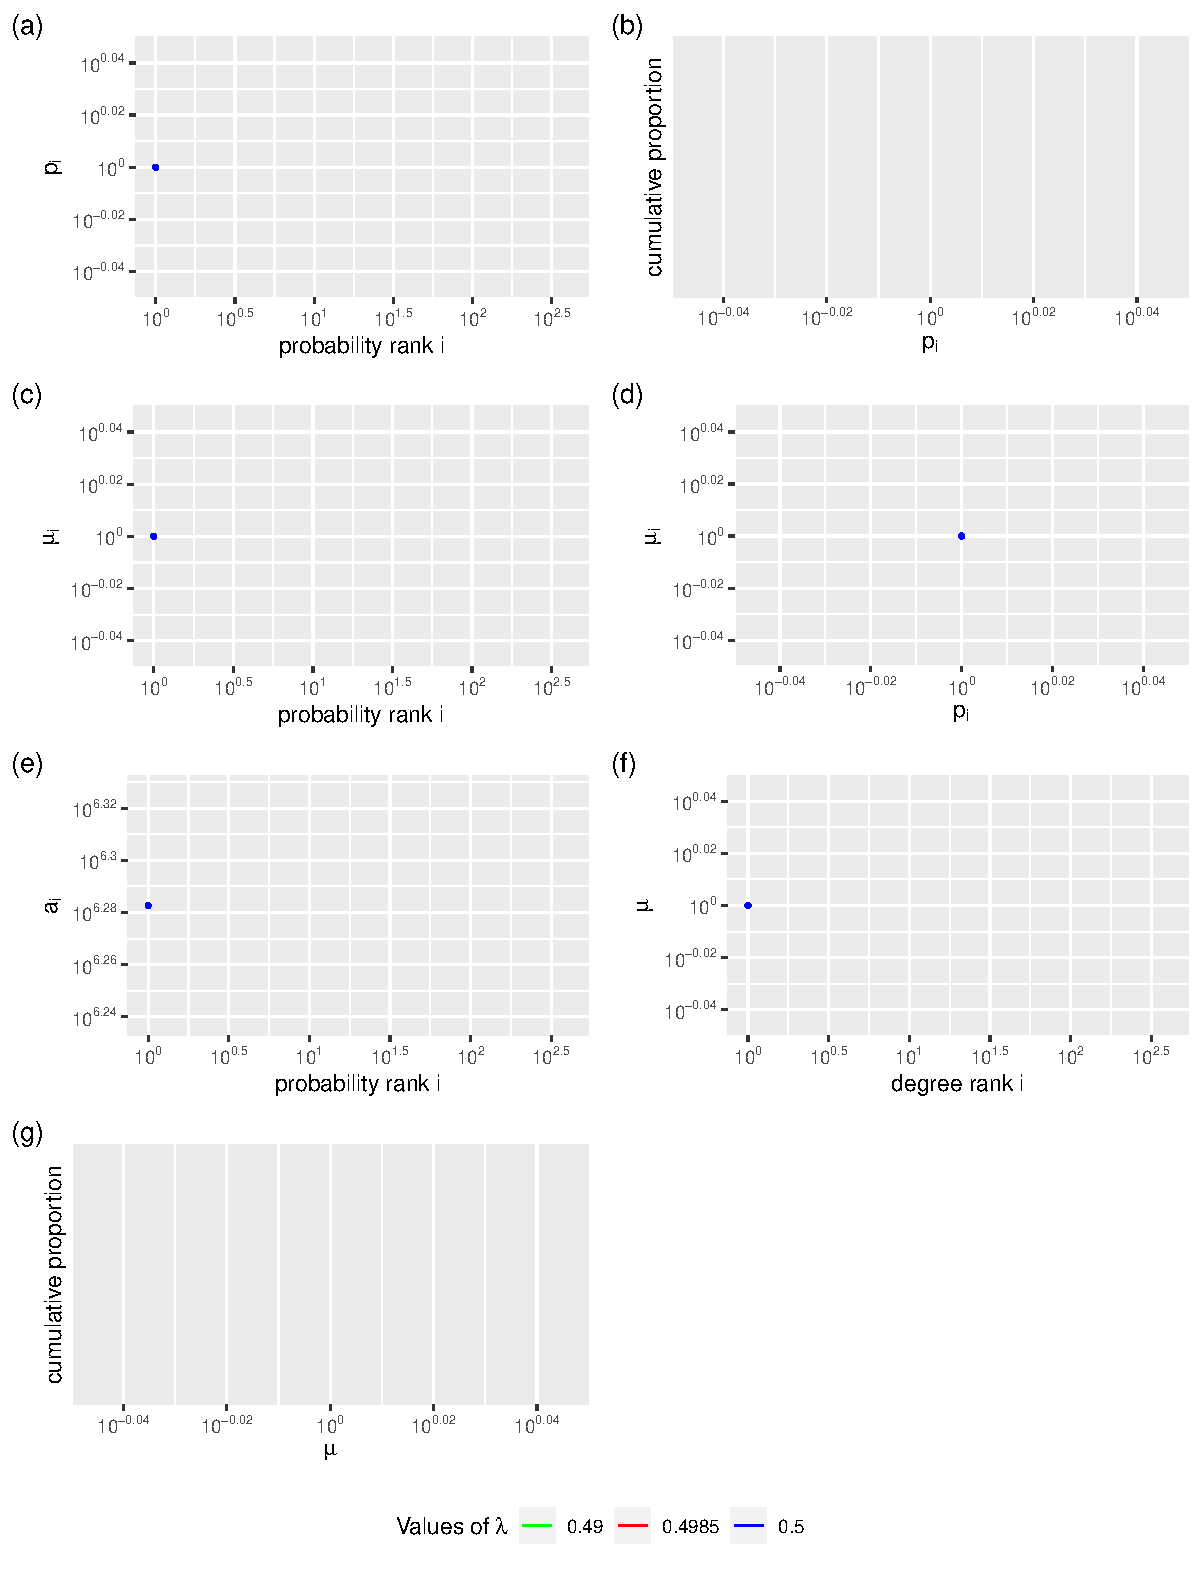
\includegraphics[width=\textwidth]{insideLambda_firstModel_phi0_nm400_dynamic_singleLink_allowUnlinked}
  \caption{a}
  \label{fig:insideLambda_firstModel_phi0_nm400_dynamic_singleLink_allowUnlinked}
\end{figure}

\begin{figure}
  \centering
  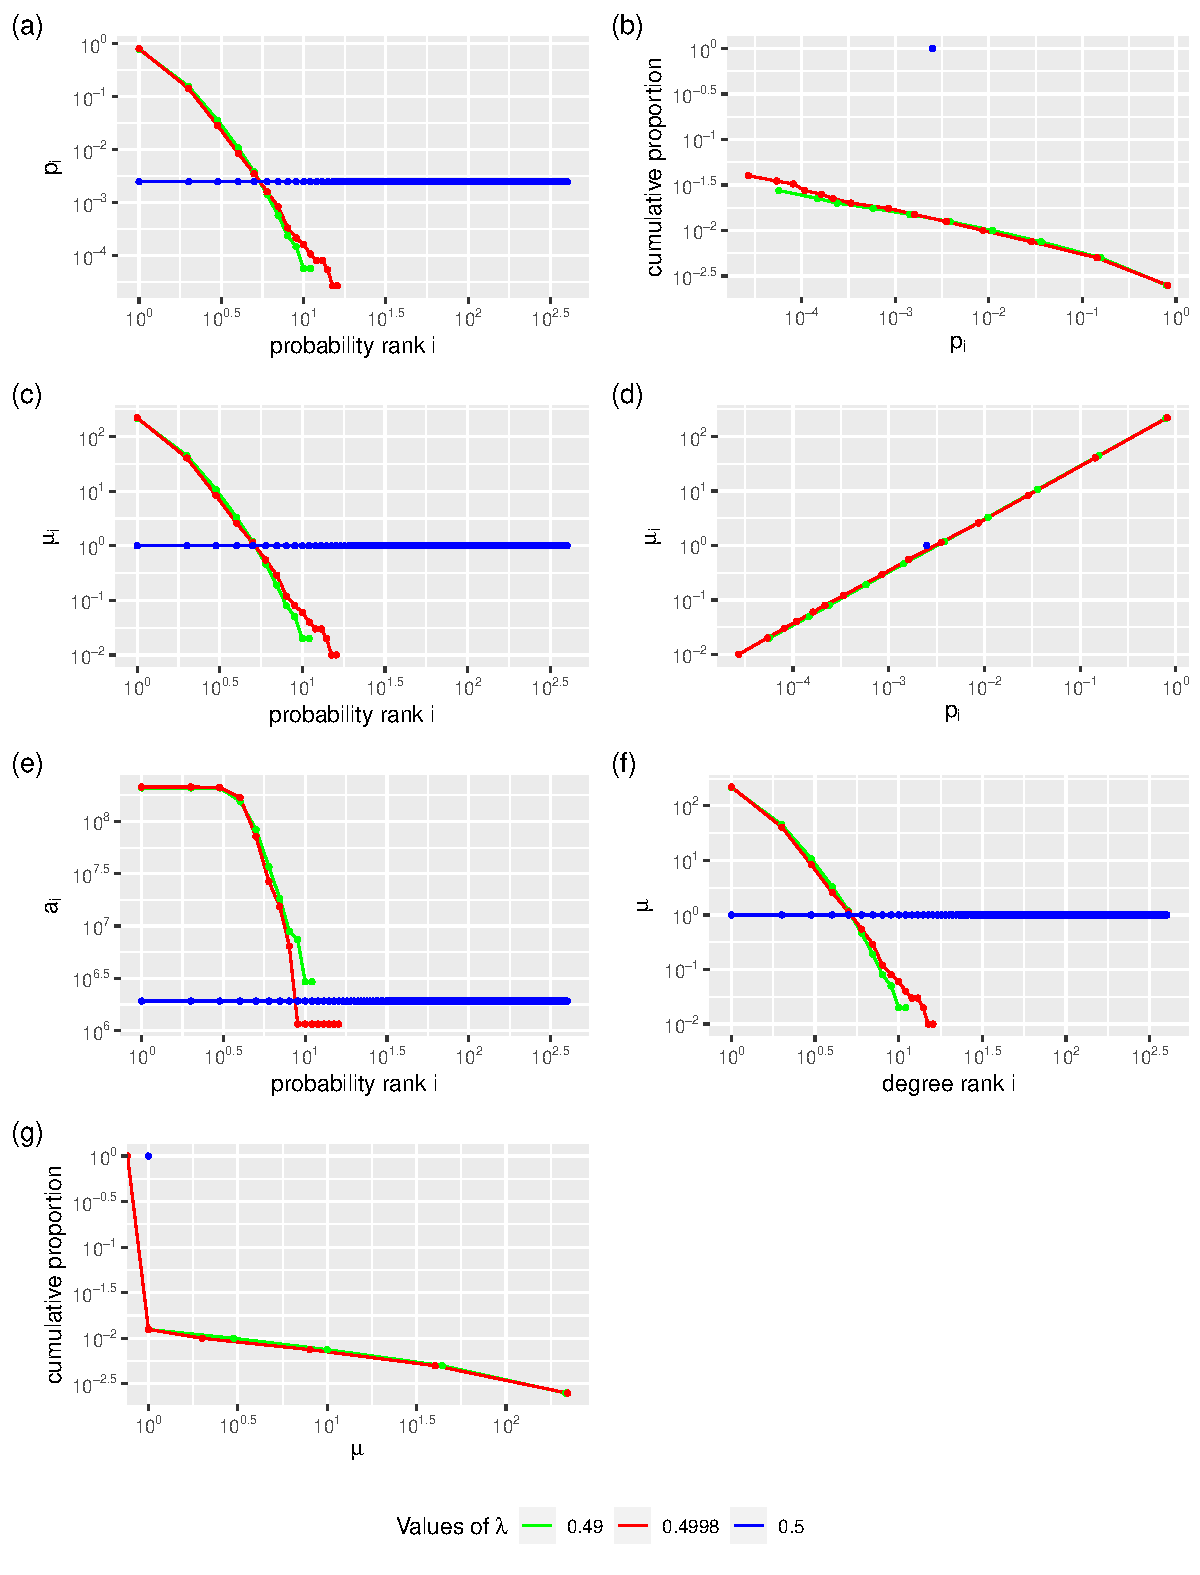
\includegraphics[width=\textwidth]{insideLambda_firstModel_phi0_nm400_dynamic_oneToOne_allowUnlinked}
  \caption{a}
  \label{fig:insideLambda_firstModel_phi0_nm400_dynamic_oneToOne_allowUnlinked}
\end{figure}

\begin{itemize}
\item initial: random \ref{fig:insideLambda_firstModel_phi0_nm400_dynamic_randomBipartite_allowUnlinked}
\item initial: single \ref{fig:insideLambda_firstModel_phi0_nm400_dynamic_singleLink_allowUnlinked}
\item initial: one-to-one \ref{fig:insideLambda_firstModel_phi0_nm400_dynamic_oneToOne_allowUnlinked}
\end{itemize}

\subsubsection{first model, $\phi=1$}

\begin{figure}
  \centering
  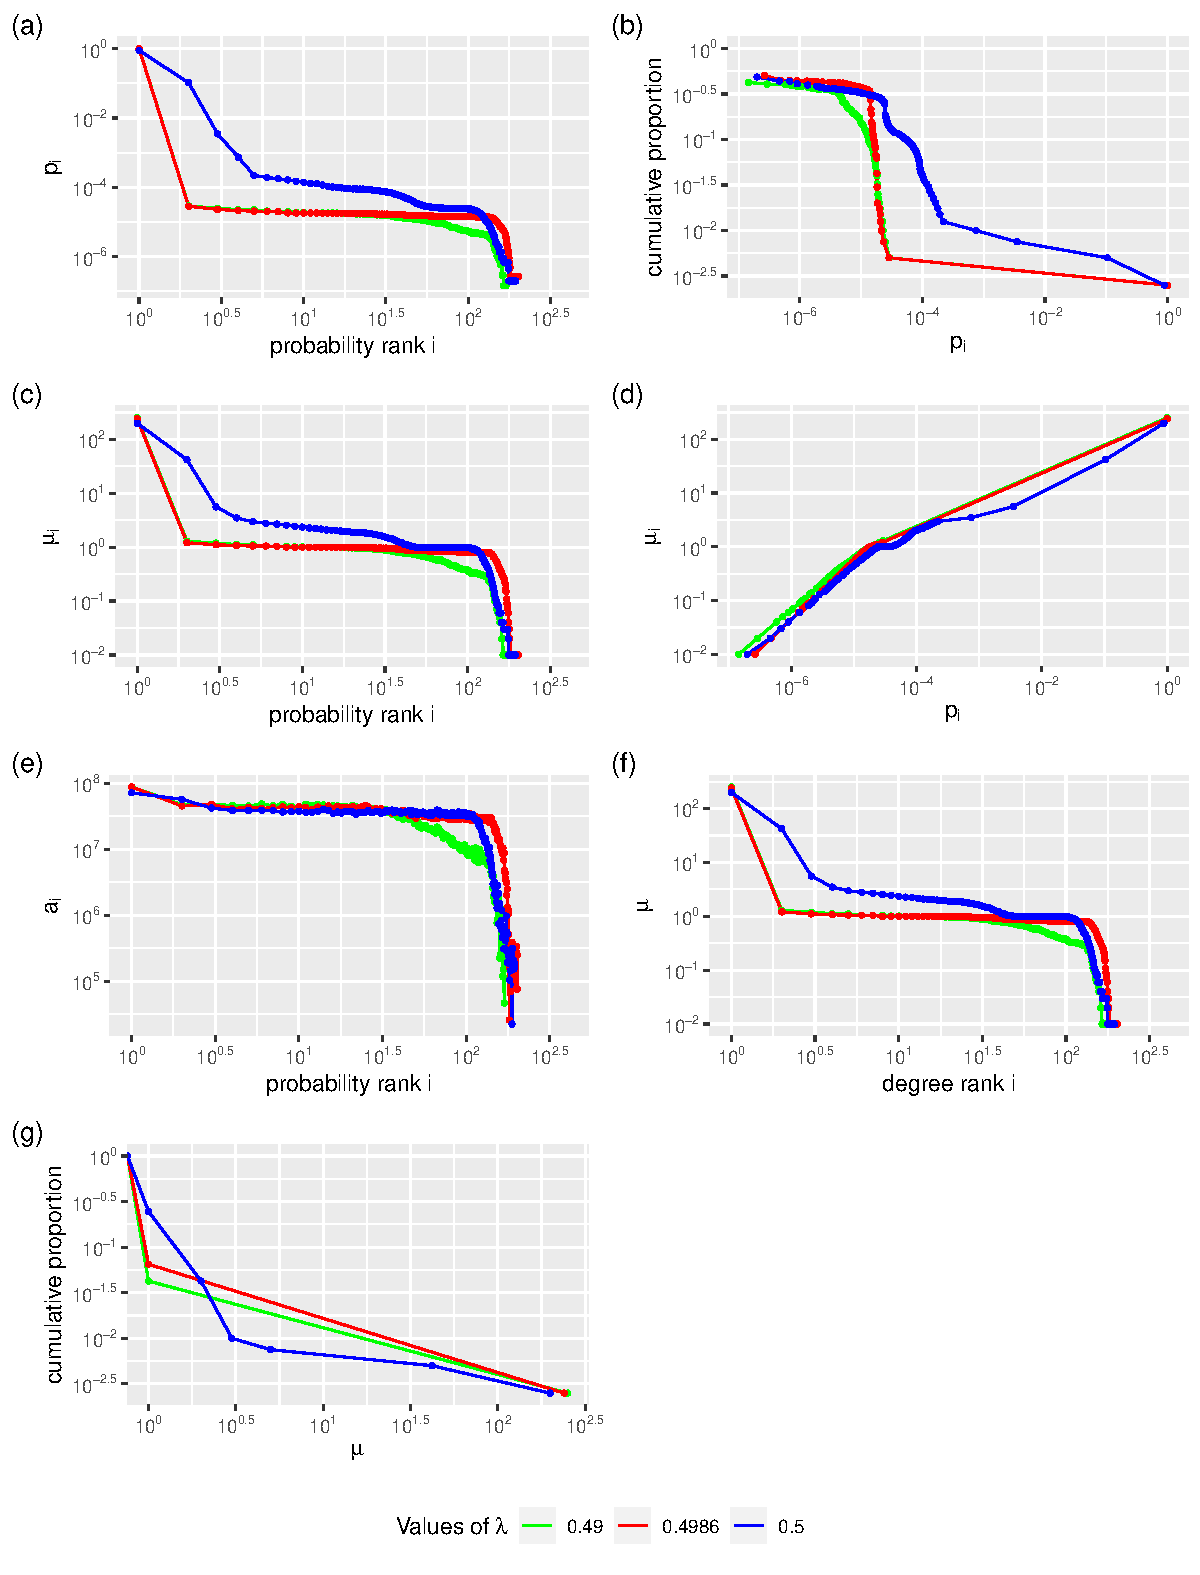
\includegraphics[width=\textwidth]{insideLambda_firstModel_phi1_nm400_dynamic_randomBipartite_allowUnlinked}
  \caption{a}
  \label{fig:insideLambda_firstModel_phi1_nm400_dynamic_randomBipartite_allowUnlinked}
\end{figure}

\begin{figure}
  \centering
  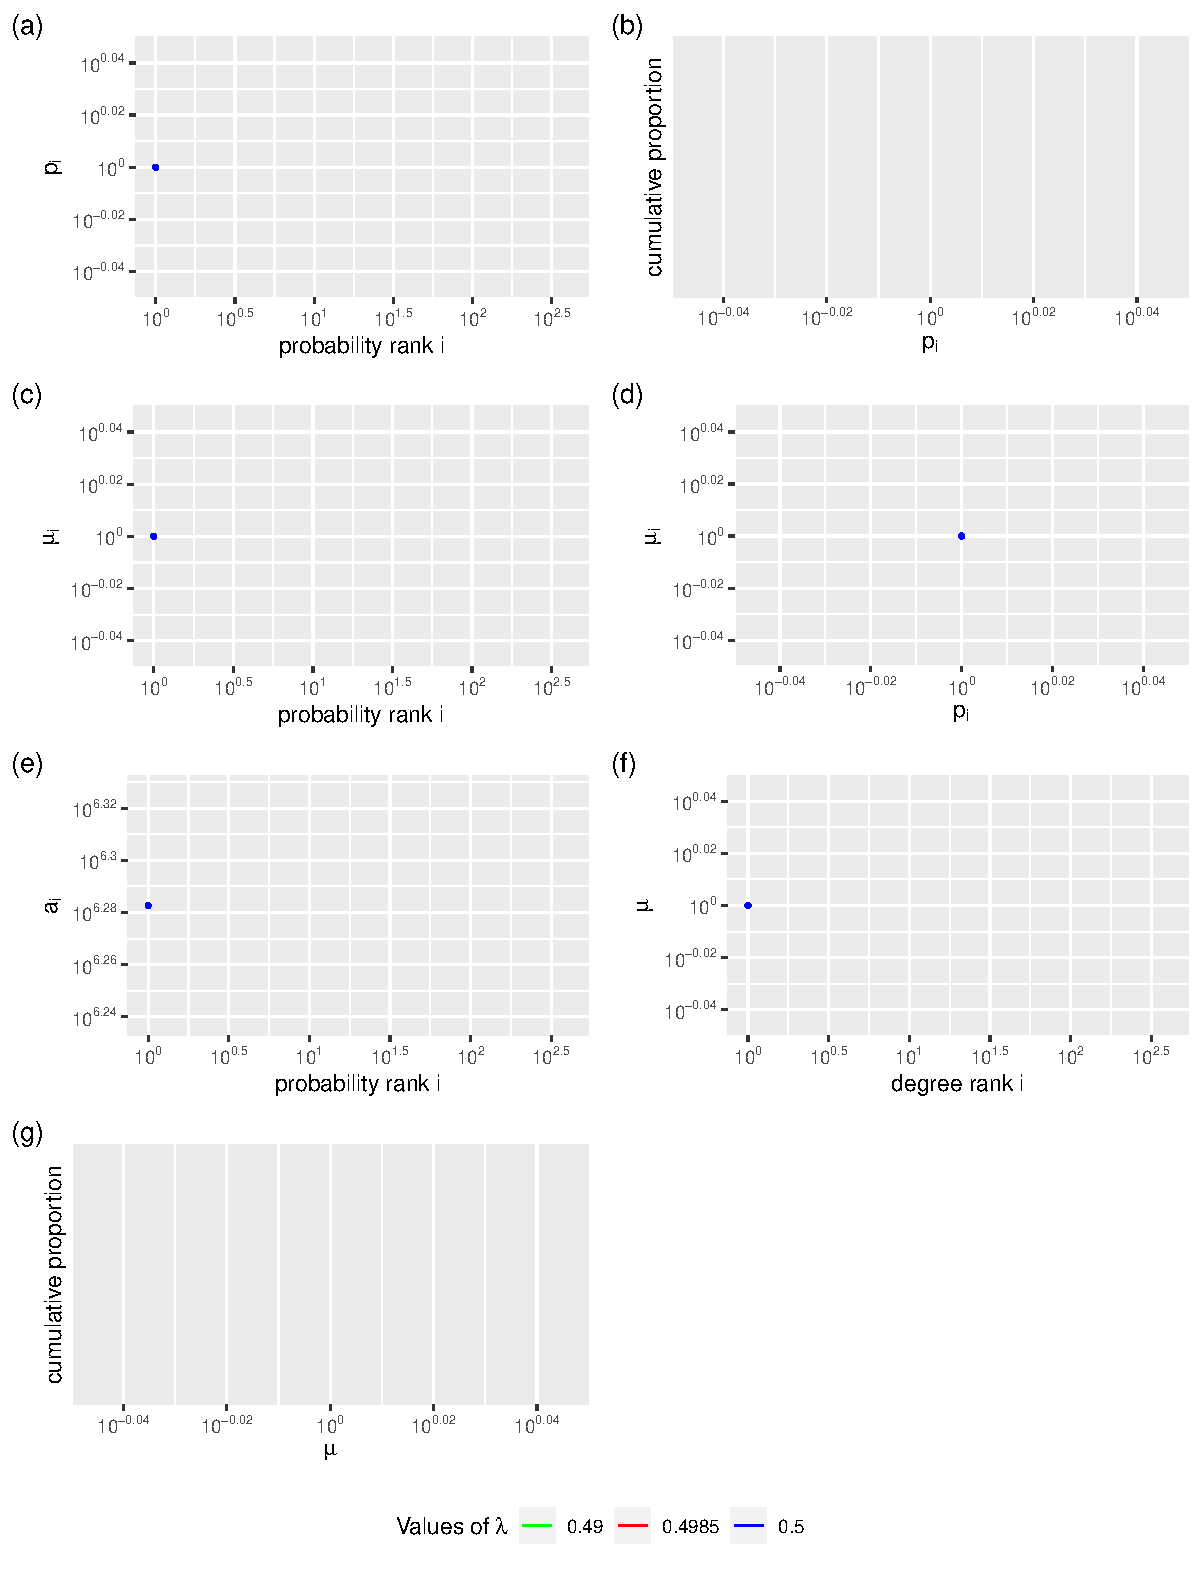
\includegraphics[width=\textwidth]{insideLambda_firstModel_phi1_nm400_dynamic_singleLink_allowUnlinked}
  \caption{a}
  \label{fig:insideLambda_firstModel_phi1_nm400_dynamic_singleLink_allowUnlinked}
\end{figure}

\begin{figure}
  \centering
  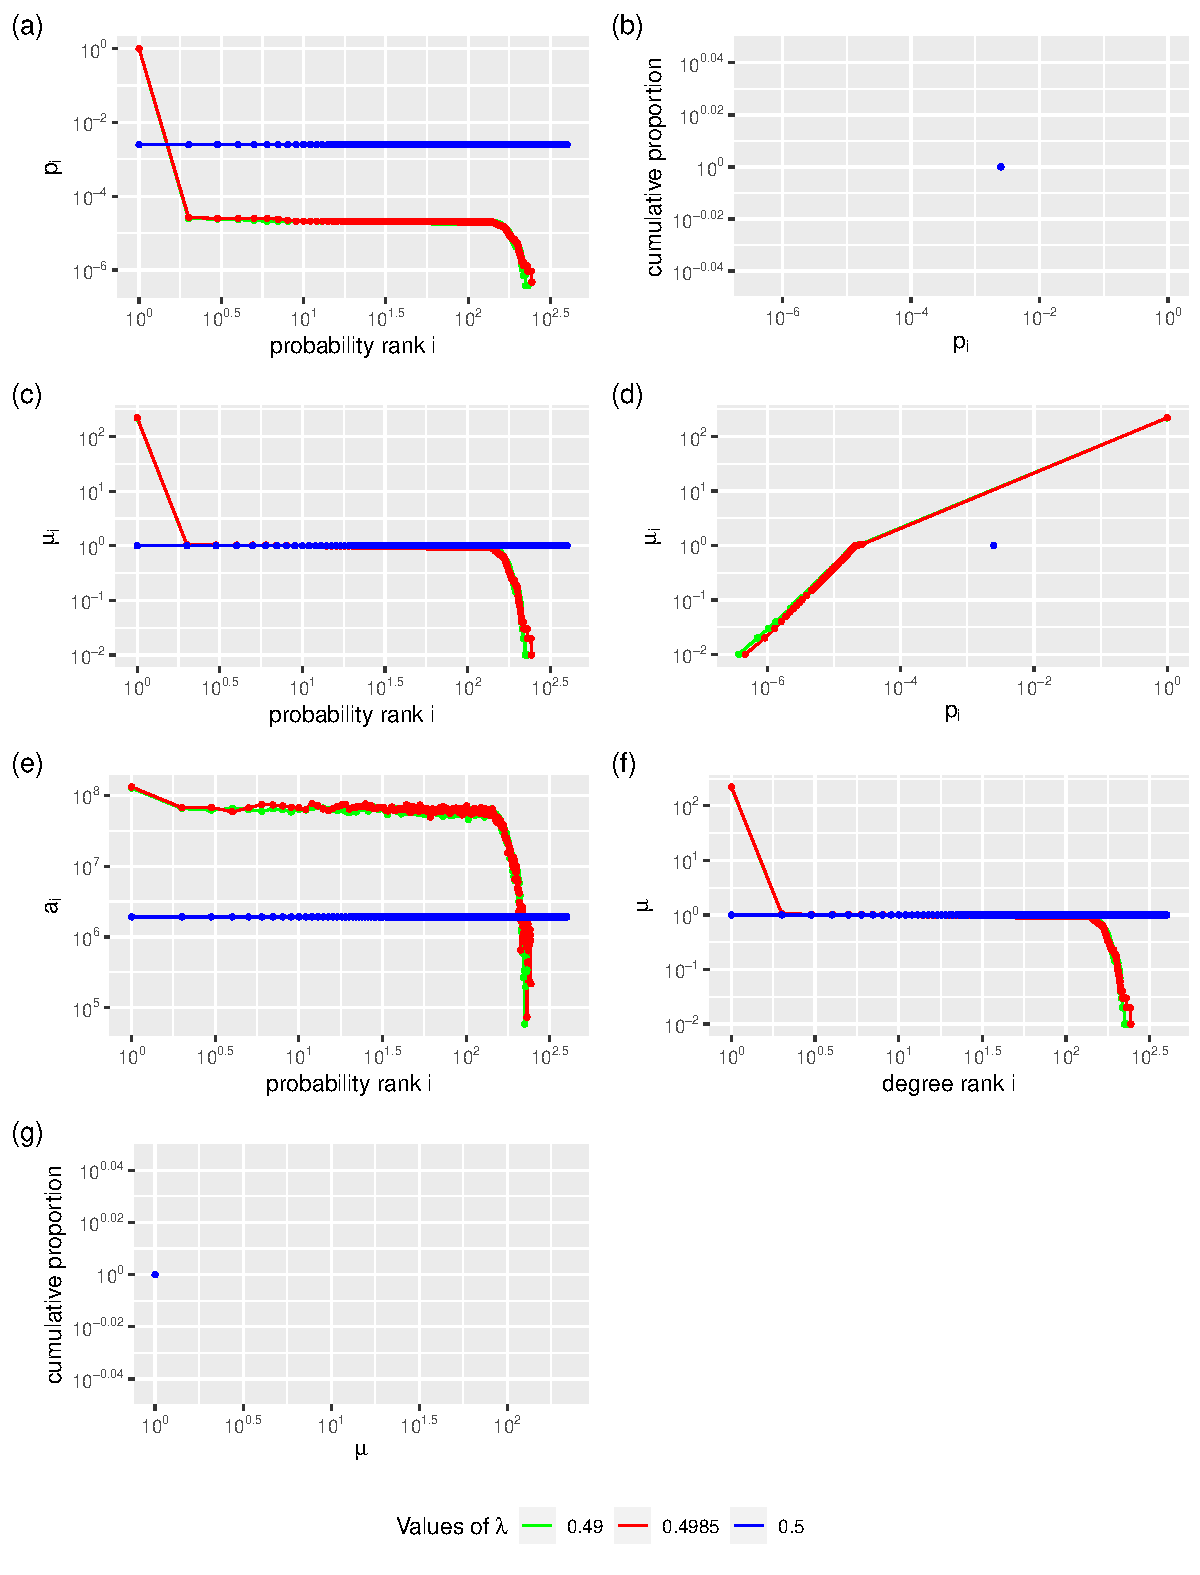
\includegraphics[width=\textwidth]{insideLambda_firstModel_phi1_nm400_dynamic_oneToOne_allowUnlinked}
  \caption{a}
  \label{fig:insideLambda_firstModel_phi1_nm400_dynamic_oneToOne_allowUnlinked}
\end{figure}

\begin{itemize}
\item initial: random \ref{fig:insideLambda_firstModel_phi1_nm400_dynamic_randomBipartite_allowUnlinked}
\item initial: single \ref{fig:insideLambda_firstModel_phi1_nm400_dynamic_singleLink_allowUnlinked}
\item initial: one-to-one \ref{fig:insideLambda_firstModel_phi1_nm400_dynamic_oneToOne_allowUnlinked}
\end{itemize}

\subsubsection{second model, $\phi=0$}

all $\pi$ uniform

\begin{figure}
  \centering
  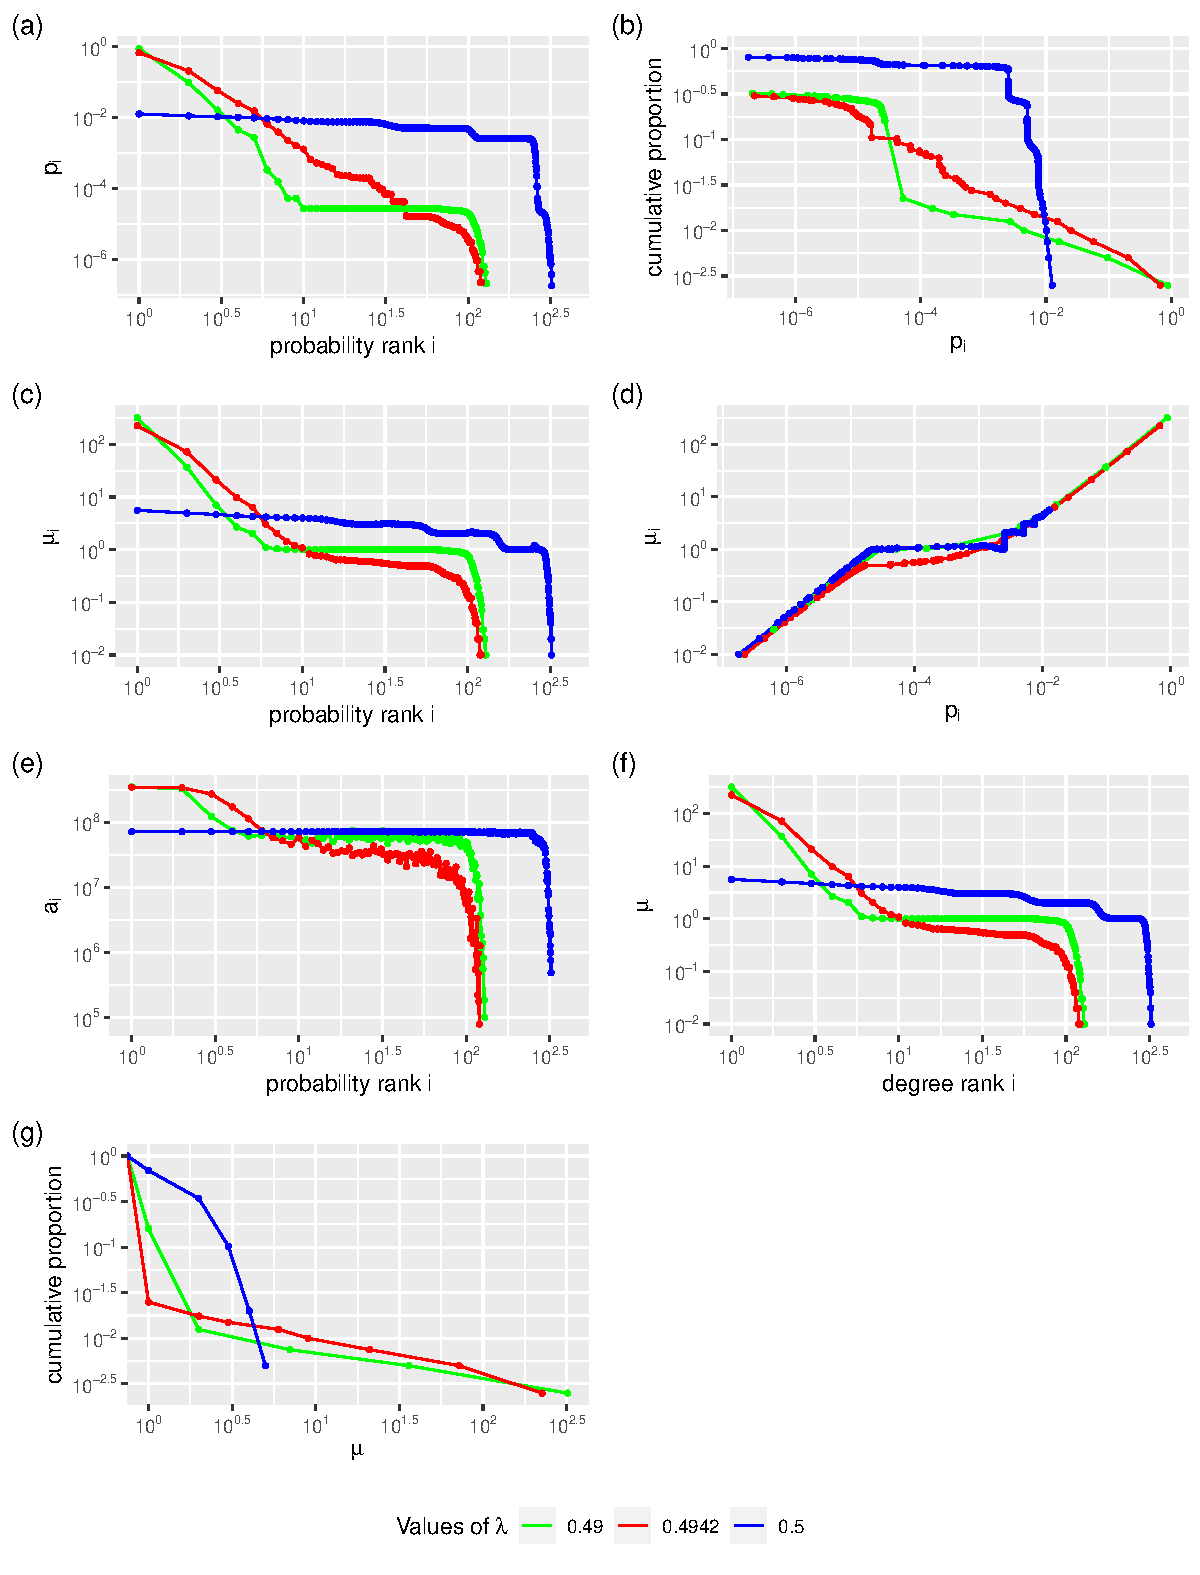
\includegraphics[width=\textwidth]{insideLambda_uniform_phi0_nm400_dynamic_randomBipartite_allowUnlinked}
  \caption{a}
  \label{fig:insideLambda_uniform_phi0_nm400_dynamic_randomBipartite_allowUnlinked}
\end{figure}

\begin{figure}
  \centering
  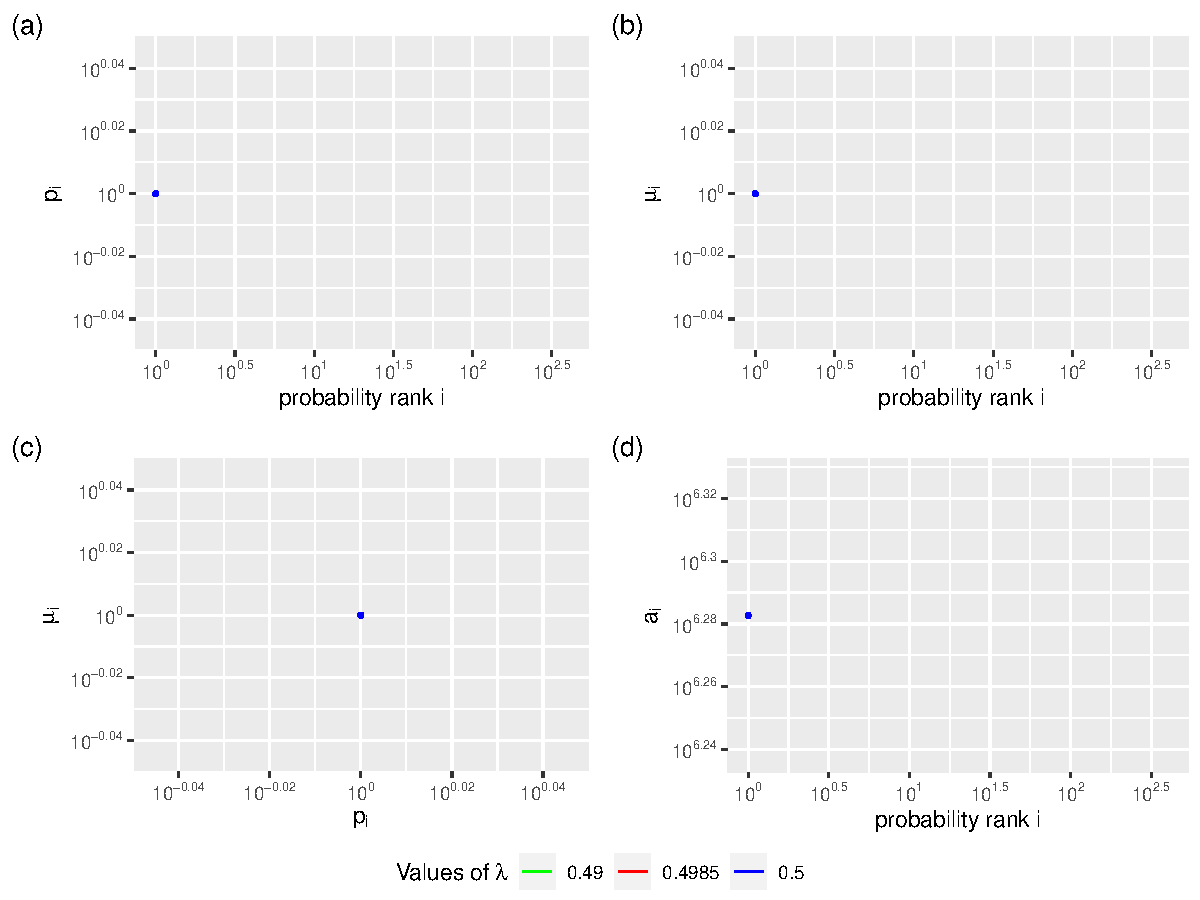
\includegraphics[width=\textwidth,draft]{insideLambda_uniform_phi0_nm400_dynamic_singleLink_allowUnlinked.pdf}
  \caption{a}
  \label{fig:insideLambda_uniform_phi0_nm400_dynamic_singleLink_allowUnlinked}
\end{figure}

\begin{figure}
  \centering
  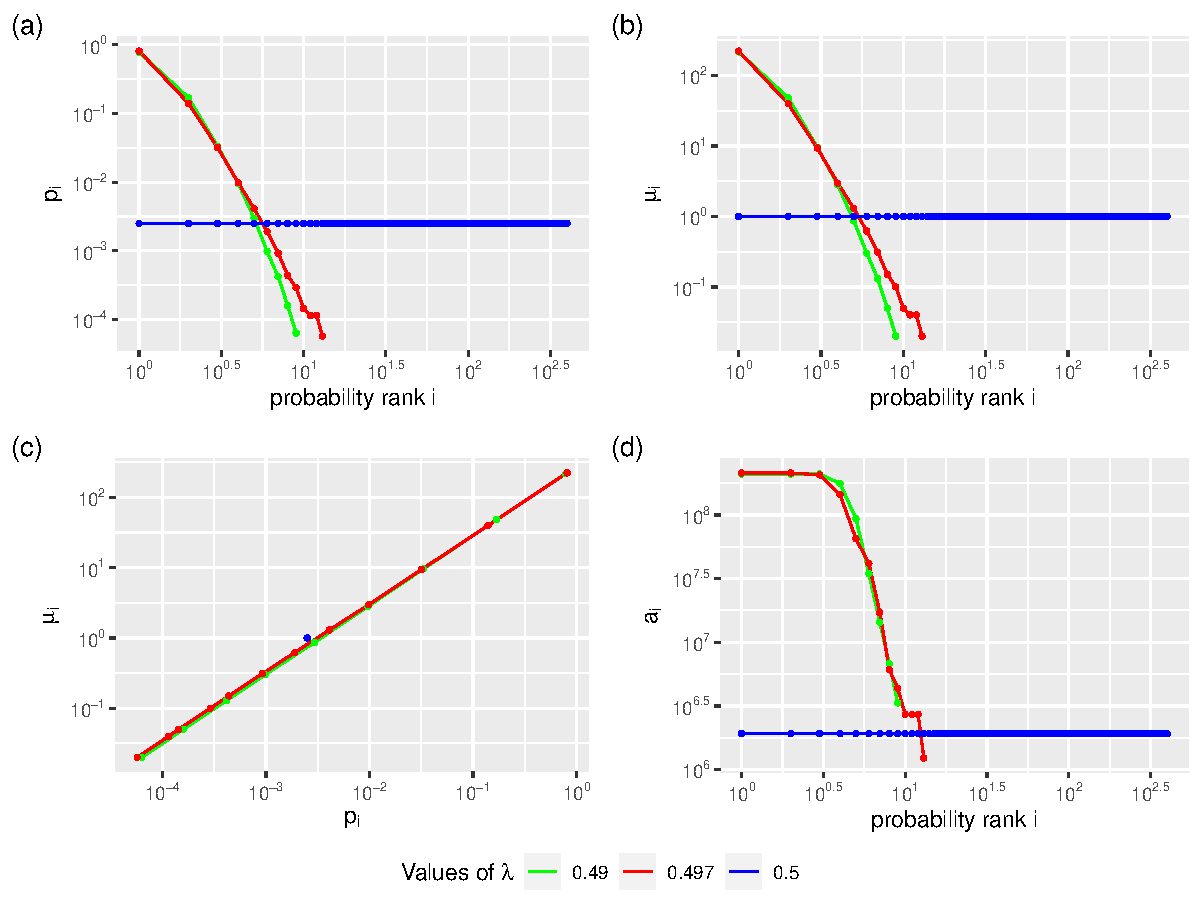
\includegraphics[width=\textwidth,draft]{insideLambda_uniform_phi0_nm400_dynamic_oneToOne_allowUnlinked.pdf}
  \caption{a}
  \label{fig:insideLambda_uniform_phi0_nm400_dynamic_oneToOne_allowUnlinked}
\end{figure}

\begin{figure}
  \centering
  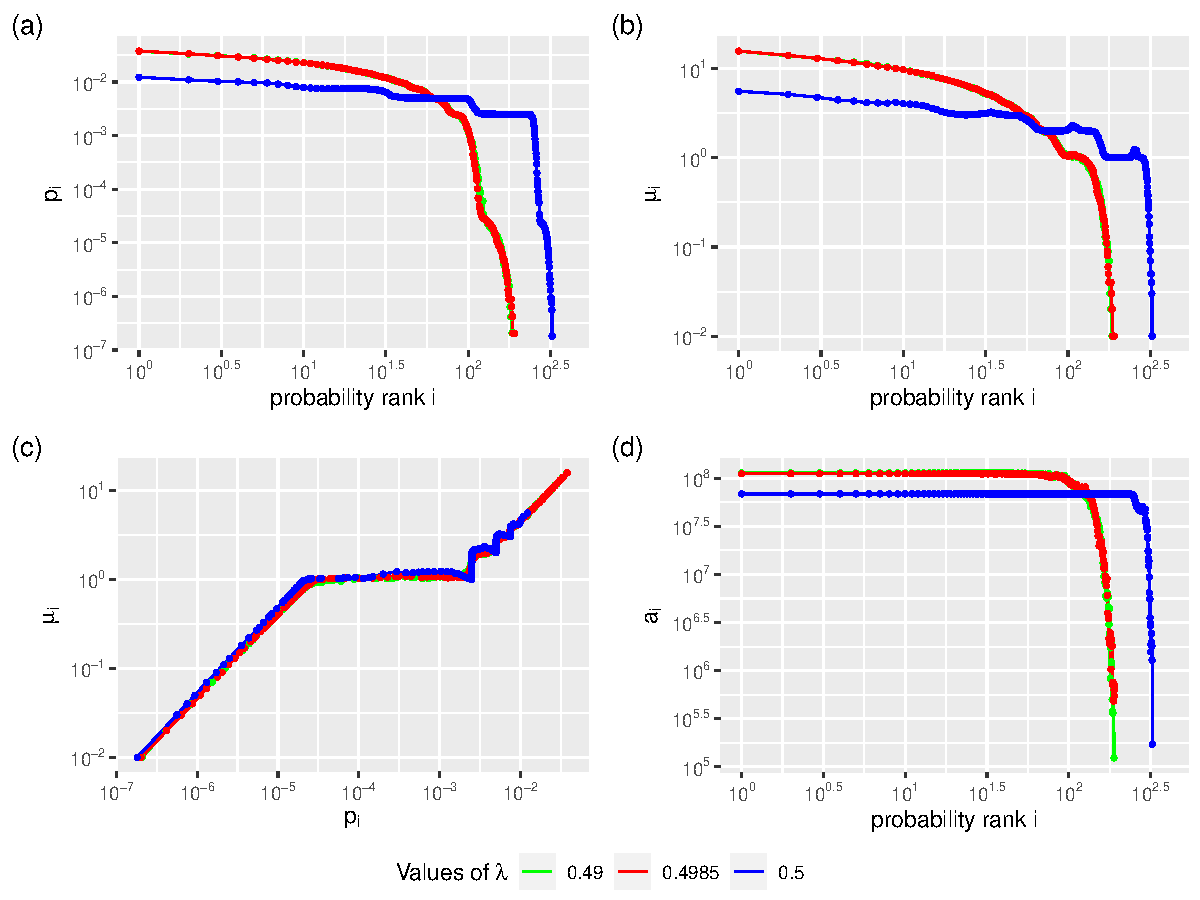
\includegraphics[width=\textwidth,draft]{insideLambda_uniform_phi0_nm400_dynamic_randomBipartite_disallowUnlinked.pdf}
  \caption{a}
  \label{fig:insideLambda_uniform_phi0_nm400_dynamic_randomBipartite_disallowUnlinked}
\end{figure}

\begin{figure}
  \centering
  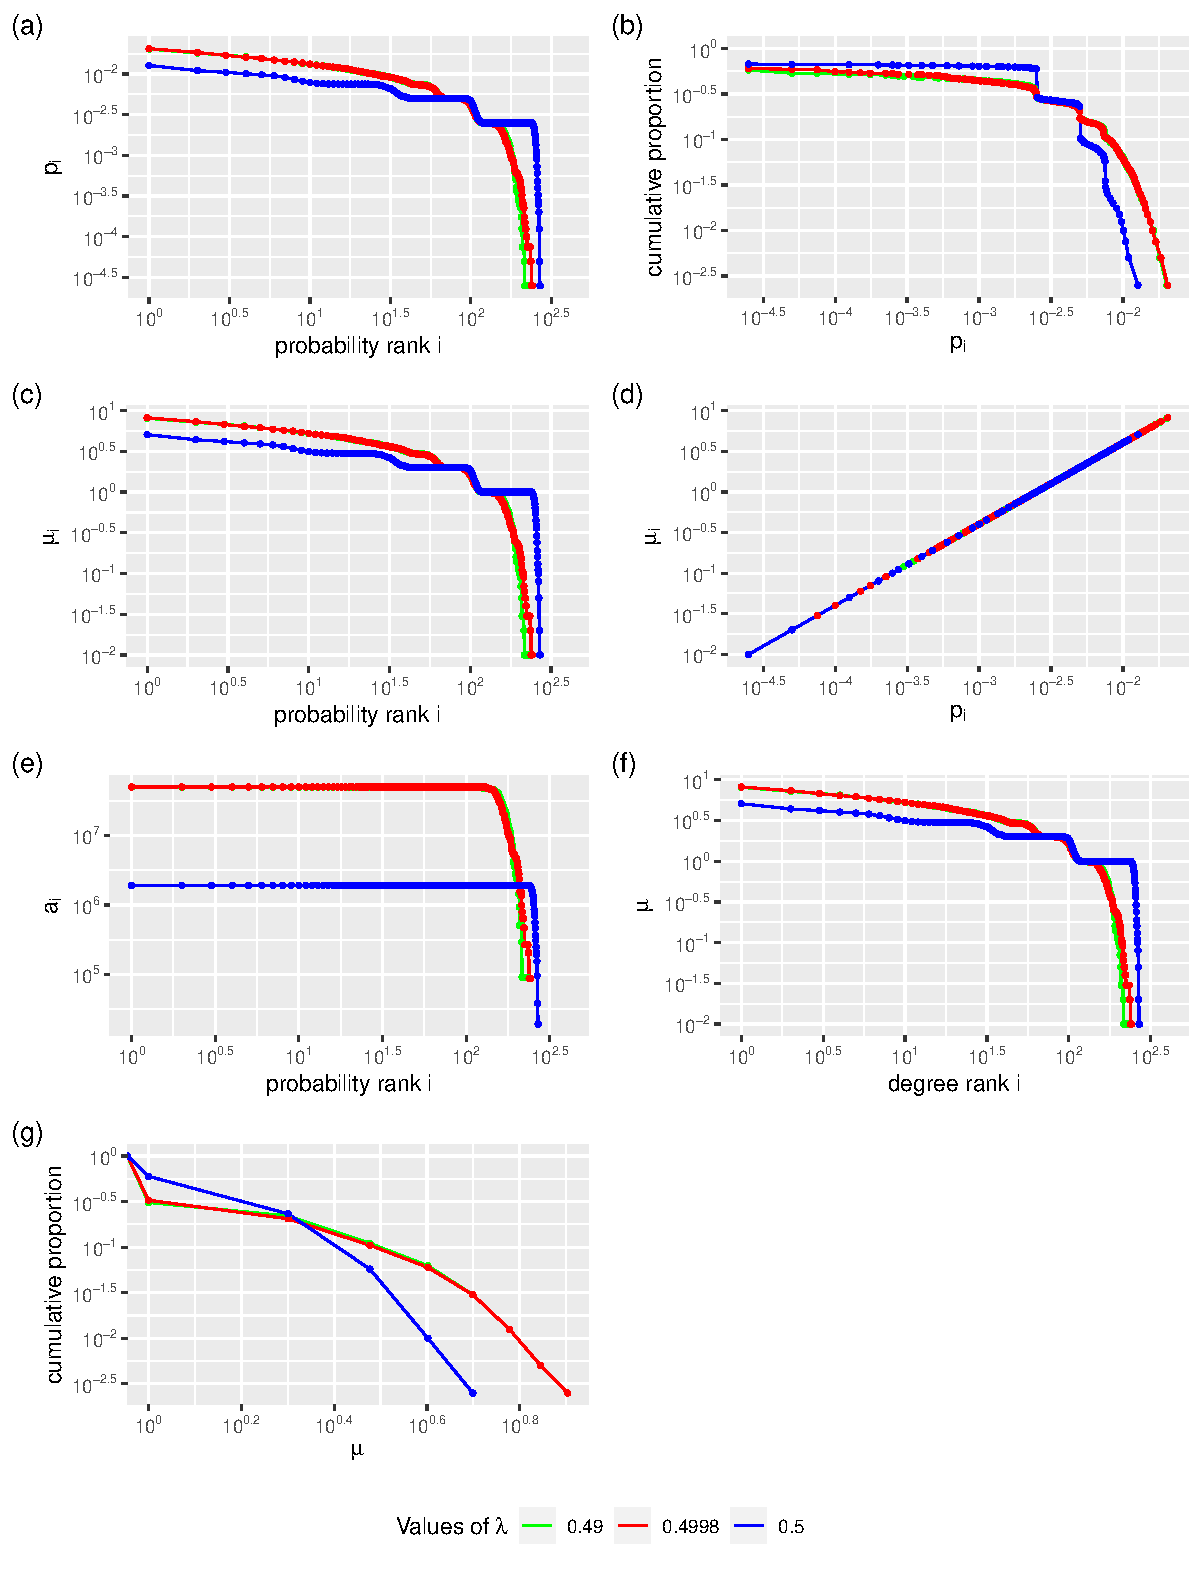
\includegraphics[width=\textwidth,draft]{insideLambda_uniform_phi0_nm400_dynamic_singleLink_disallowUnlinked.pdf}
  \caption{a}
  \label{fig:insideLambda_uniform_phi0_nm400_dynamic_singleLink_disallowUnlinked}
\end{figure}

\begin{figure}
  \centering
  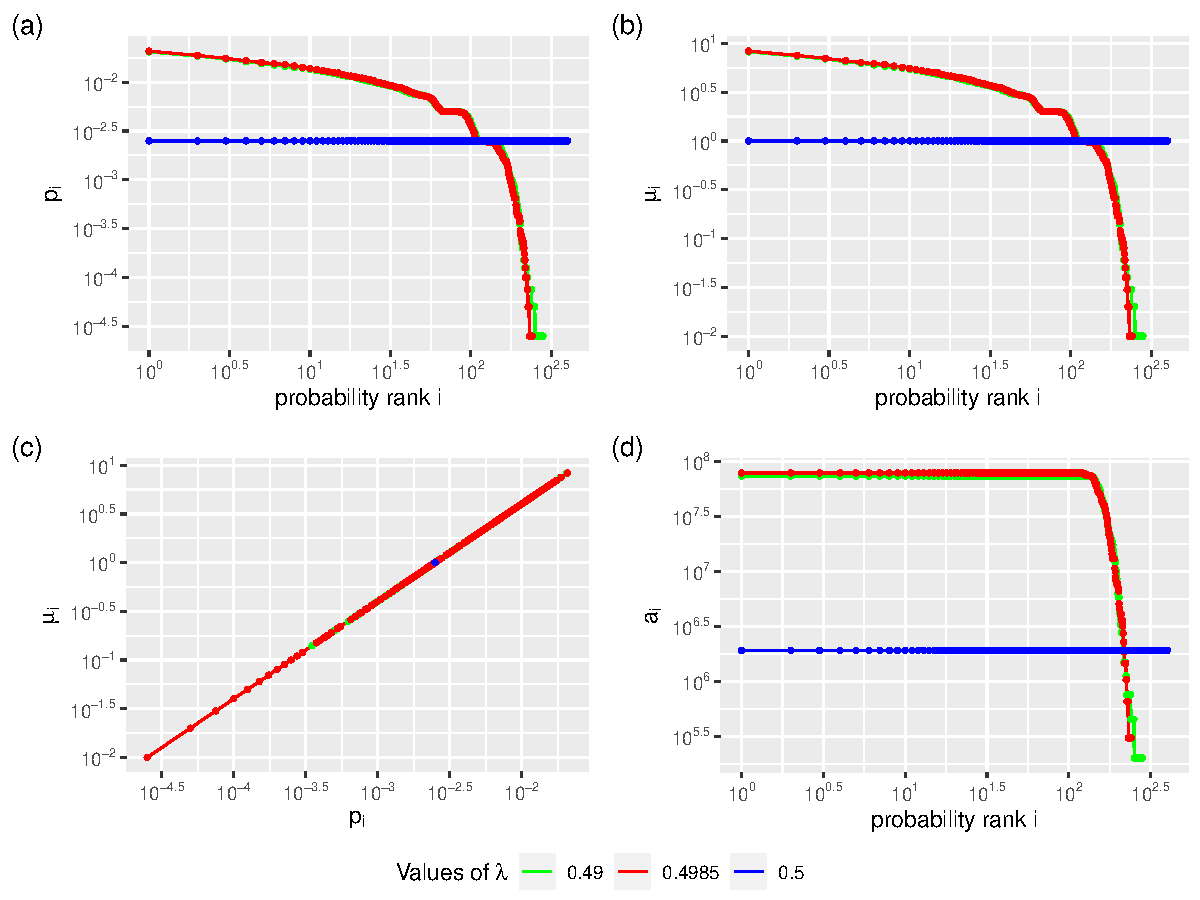
\includegraphics[width=\textwidth,draft]{insideLambda_uniform_phi0_nm400_dynamic_oneToOne_disallowUnlinked.pdf}
  \caption{a}
  \label{fig:insideLambda_uniform_phi0_nm400_dynamic_oneToOne_disallowUnlinked}
\end{figure}

\begin{itemize}
\item allow disconnect meanings
  \begin{itemize}
  \item initial: random \ref{fig:insideLambda_uniform_phi0_nm400_dynamic_randomBipartite_allowUnlinked}
  \item initial: single \ref{fig:insideLambda_uniform_phi0_nm400_dynamic_singleLink_allowUnlinked}
  \item initial: one-to-one \ref{fig:insideLambda_uniform_phi0_nm400_dynamic_oneToOne_allowUnlinked}
  \end{itemize}
\item do not allow disconnect meanings
  \begin{itemize}
  \item initial: random \ref{fig:insideLambda_uniform_phi0_nm400_dynamic_randomBipartite_disallowUnlinked}
  \item initial: single \ref{fig:insideLambda_uniform_phi0_nm400_dynamic_singleLink_disallowUnlinked}
  \item initial: one-to-one \ref{fig:insideLambda_uniform_phi0_nm400_dynamic_oneToOne_disallowUnlinked}
  \end{itemize}
\end{itemize}

\subsubsection{second model, $\phi=1$}

\begin{figure}
  \centering
  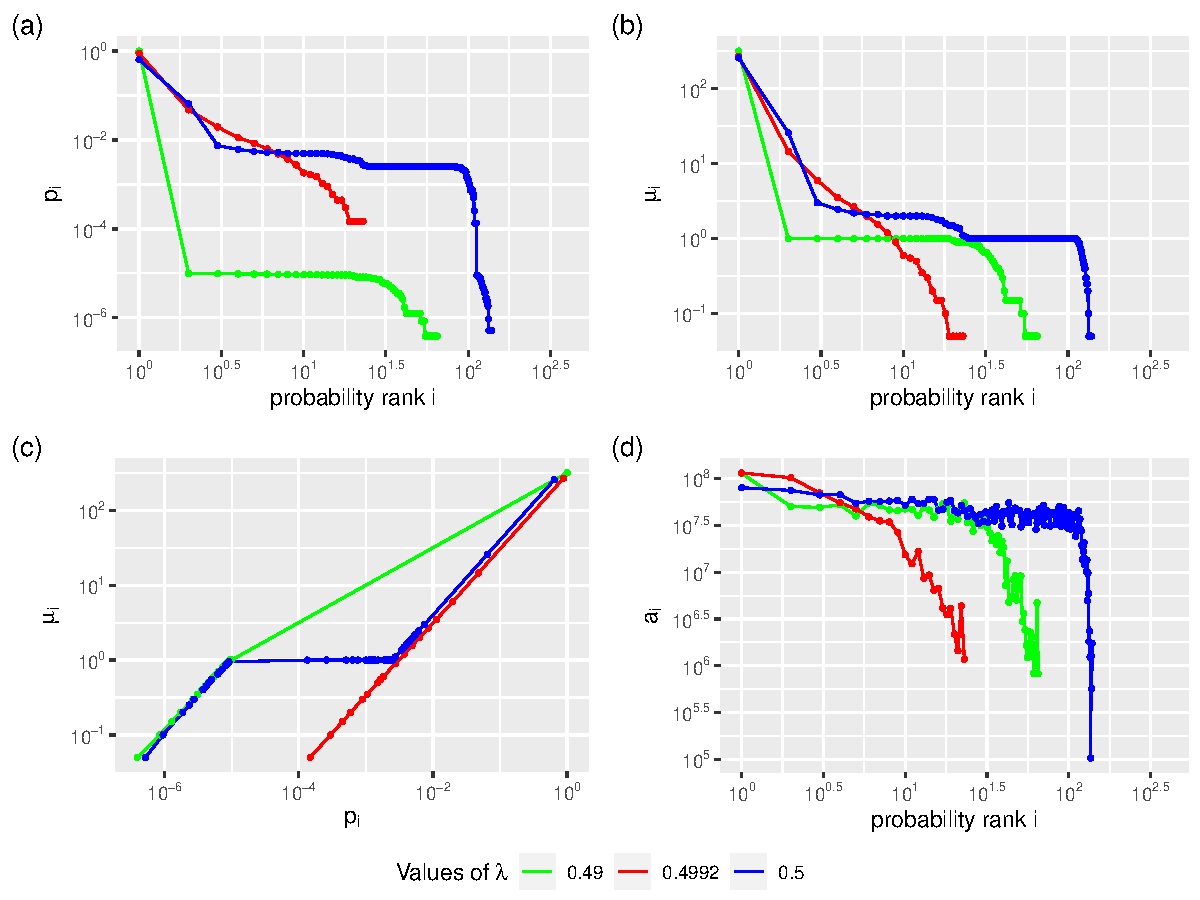
\includegraphics[width=\textwidth,draft]{insideLambda_uniform_phi1_nm400_dynamic_randomBipartite_allowUnlinked.pdf}
  \caption{a}
  \label{fig:insideLambda_uniform_phi1_nm400_dynamic_randomBipartite_allowUnlinked}
\end{figure}

\begin{figure}
  \centering
  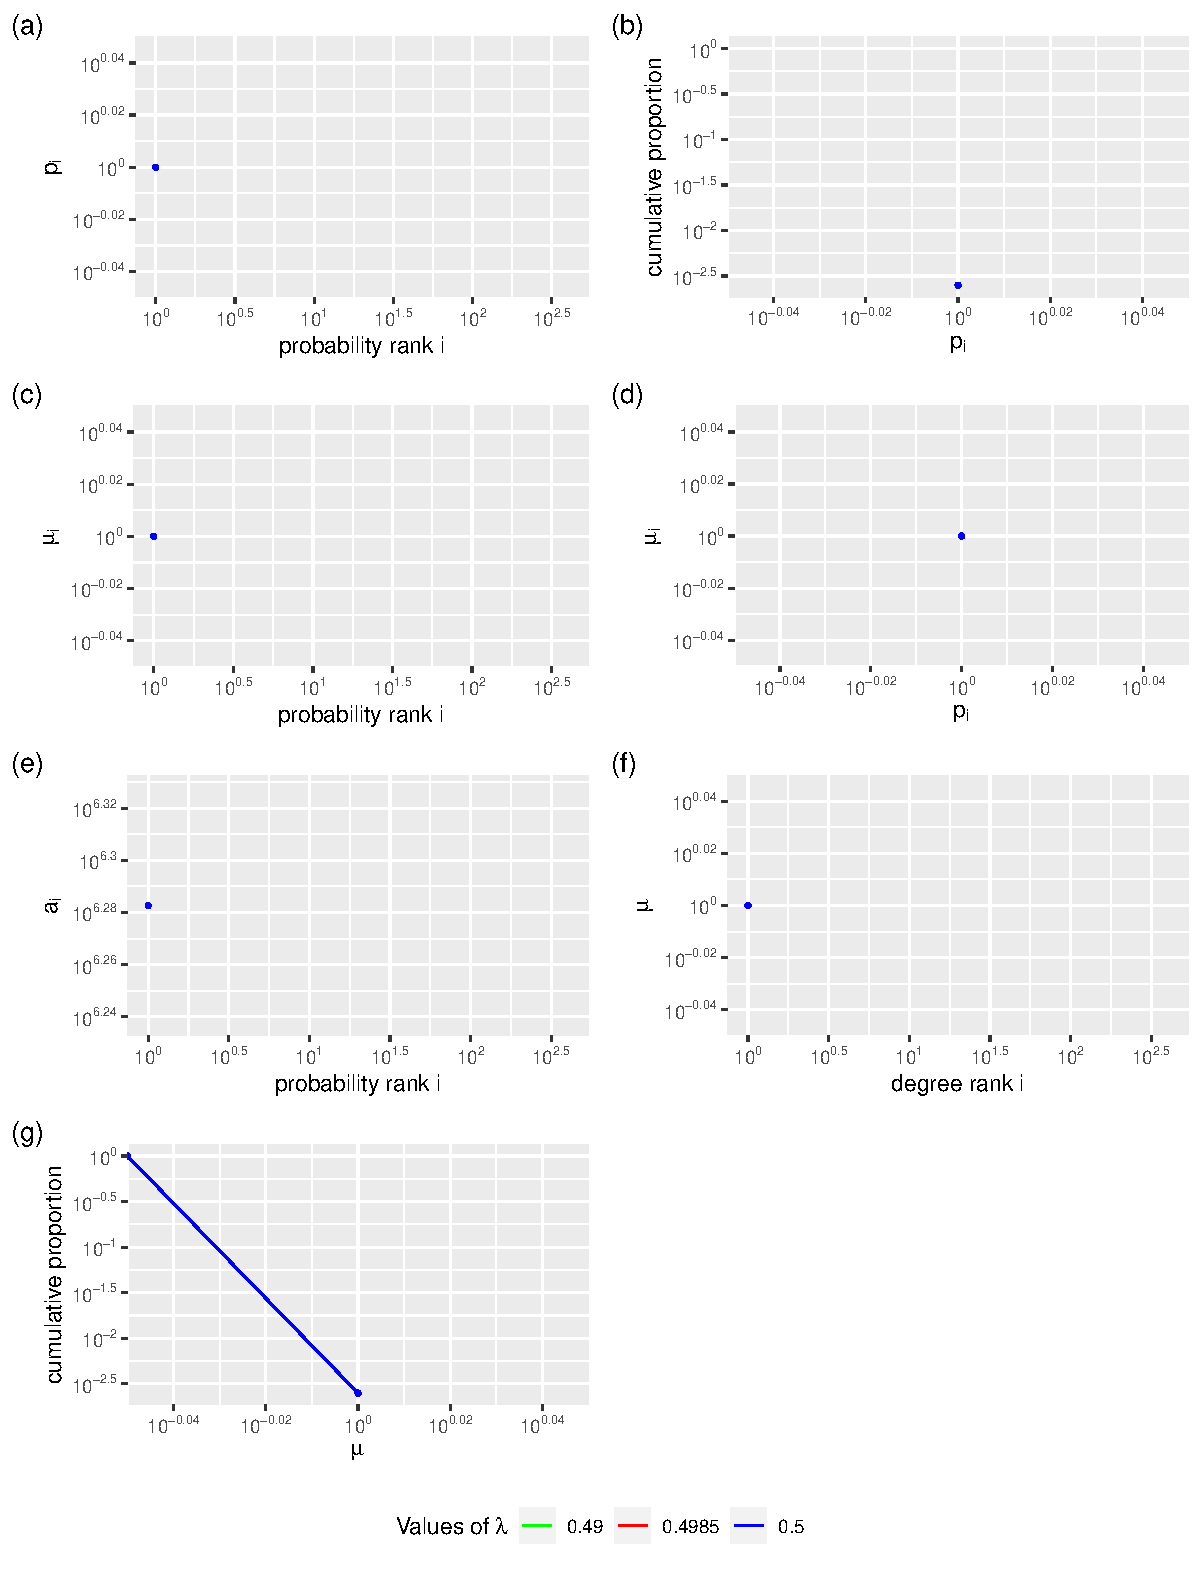
\includegraphics[width=\textwidth,draft]{insideLambda_uniform_phi1_nm400_dynamic_singleLink_allowUnlinked.pdf}
  \caption{a}
  \label{fig:insideLambda_uniform_phi1_nm400_dynamic_singleLink_allowUnlinked}
\end{figure}

\begin{figure}
  \centering
  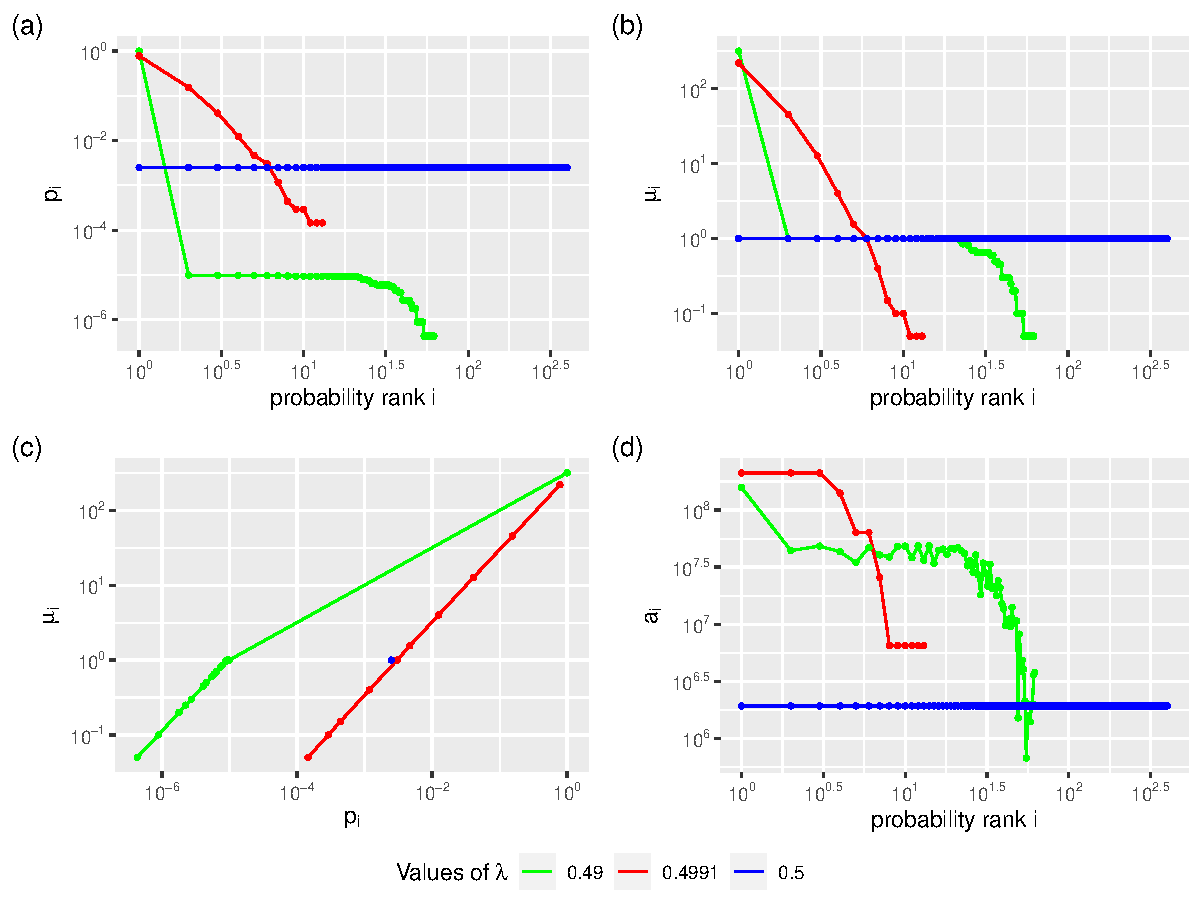
\includegraphics[width=\textwidth,draft]{insideLambda_uniform_phi1_nm400_dynamic_oneToOne_allowUnlinked.pdf}
  \caption{a}
  \label{fig:insideLambda_uniform_phi1_nm400_dynamic_oneToOne_allowUnlinked}
\end{figure}

\begin{figure}
  \centering
  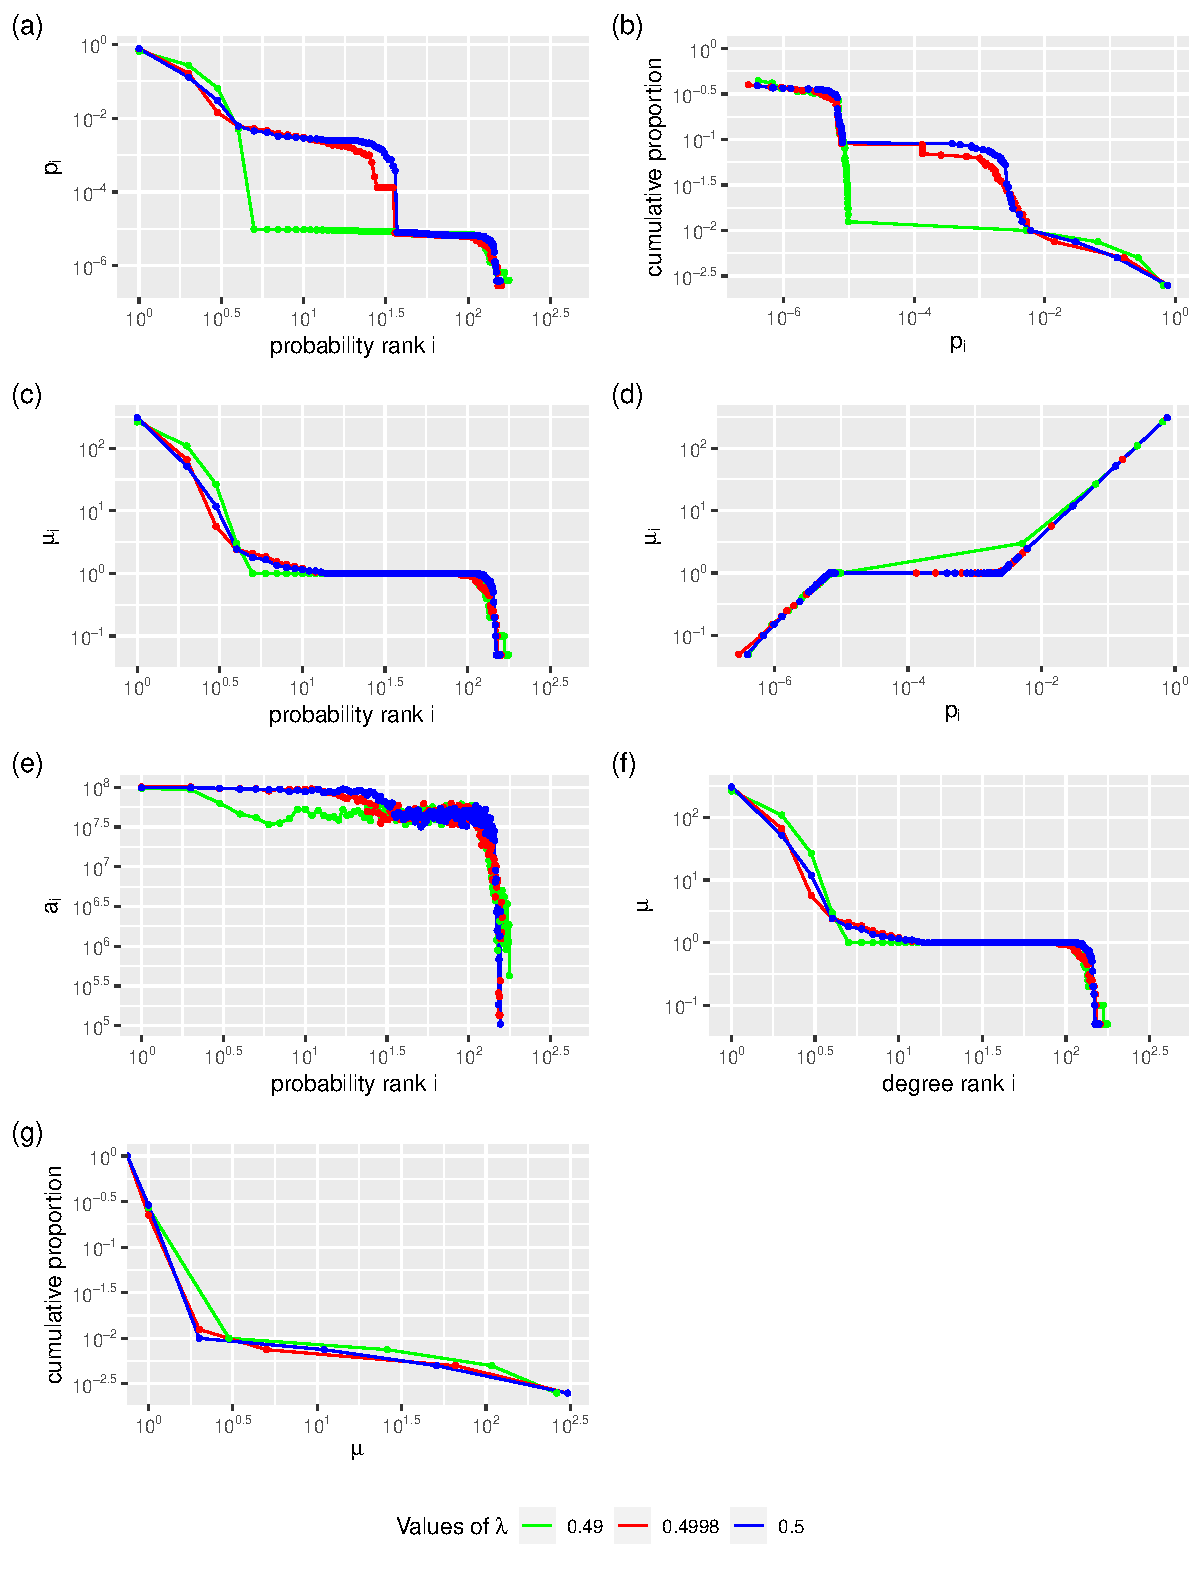
\includegraphics[width=\textwidth,draft]{insideLambda_uniform_phi1_nm400_dynamic_randomBipartite_disallowUnlinked.pdf}
  \caption{a}
  \label{fig:insideLambda_uniform_phi1_nm400_dynamic_randomBipartite_disallowUnlinked}
\end{figure}

\begin{figure}
  \centering
  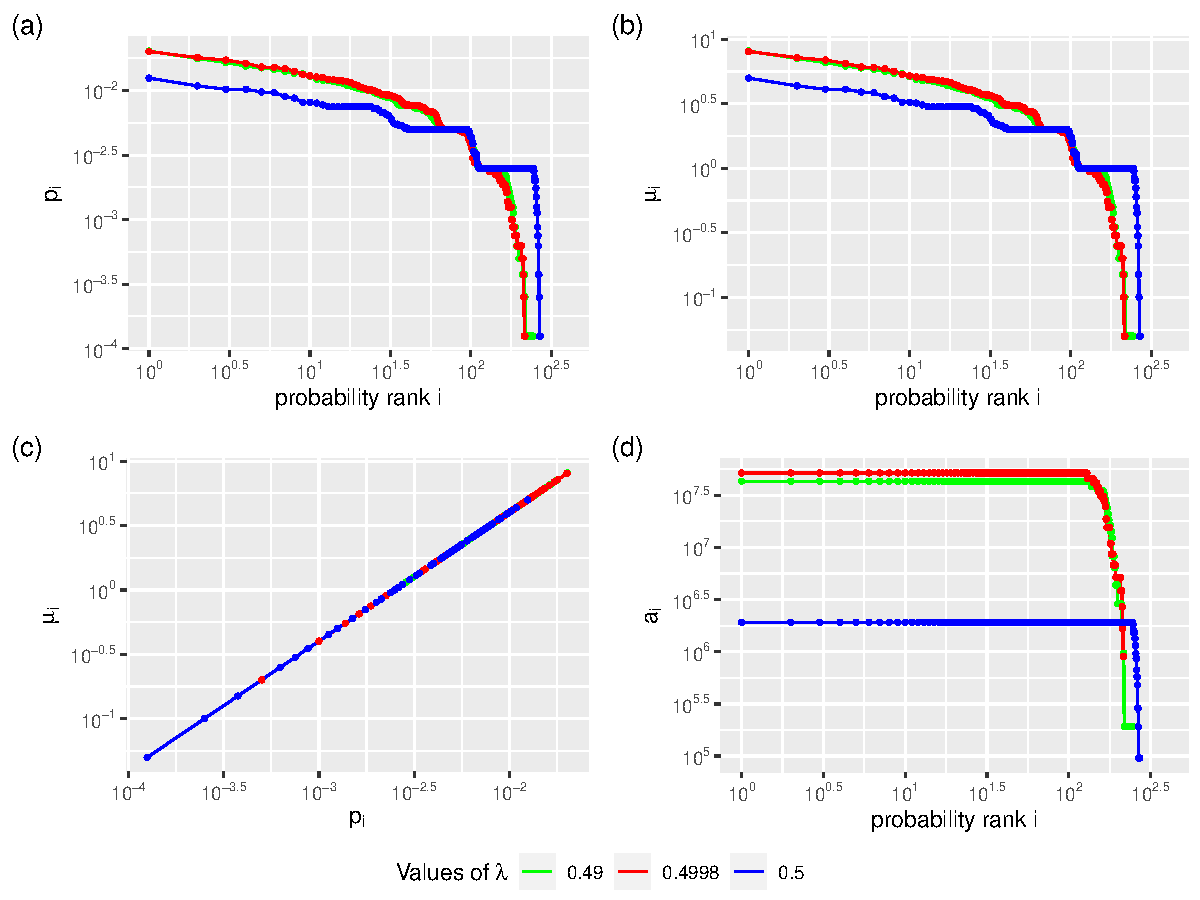
\includegraphics[width=\textwidth,draft]{insideLambda_uniform_phi1_nm400_dynamic_singleLink_disallowUnlinked.pdf}
  \caption{a}
  \label{fig:insideLambda_uniform_phi1_nm400_dynamic_singleLink_disallowUnlinked}
\end{figure}

\begin{figure}
  \centering
  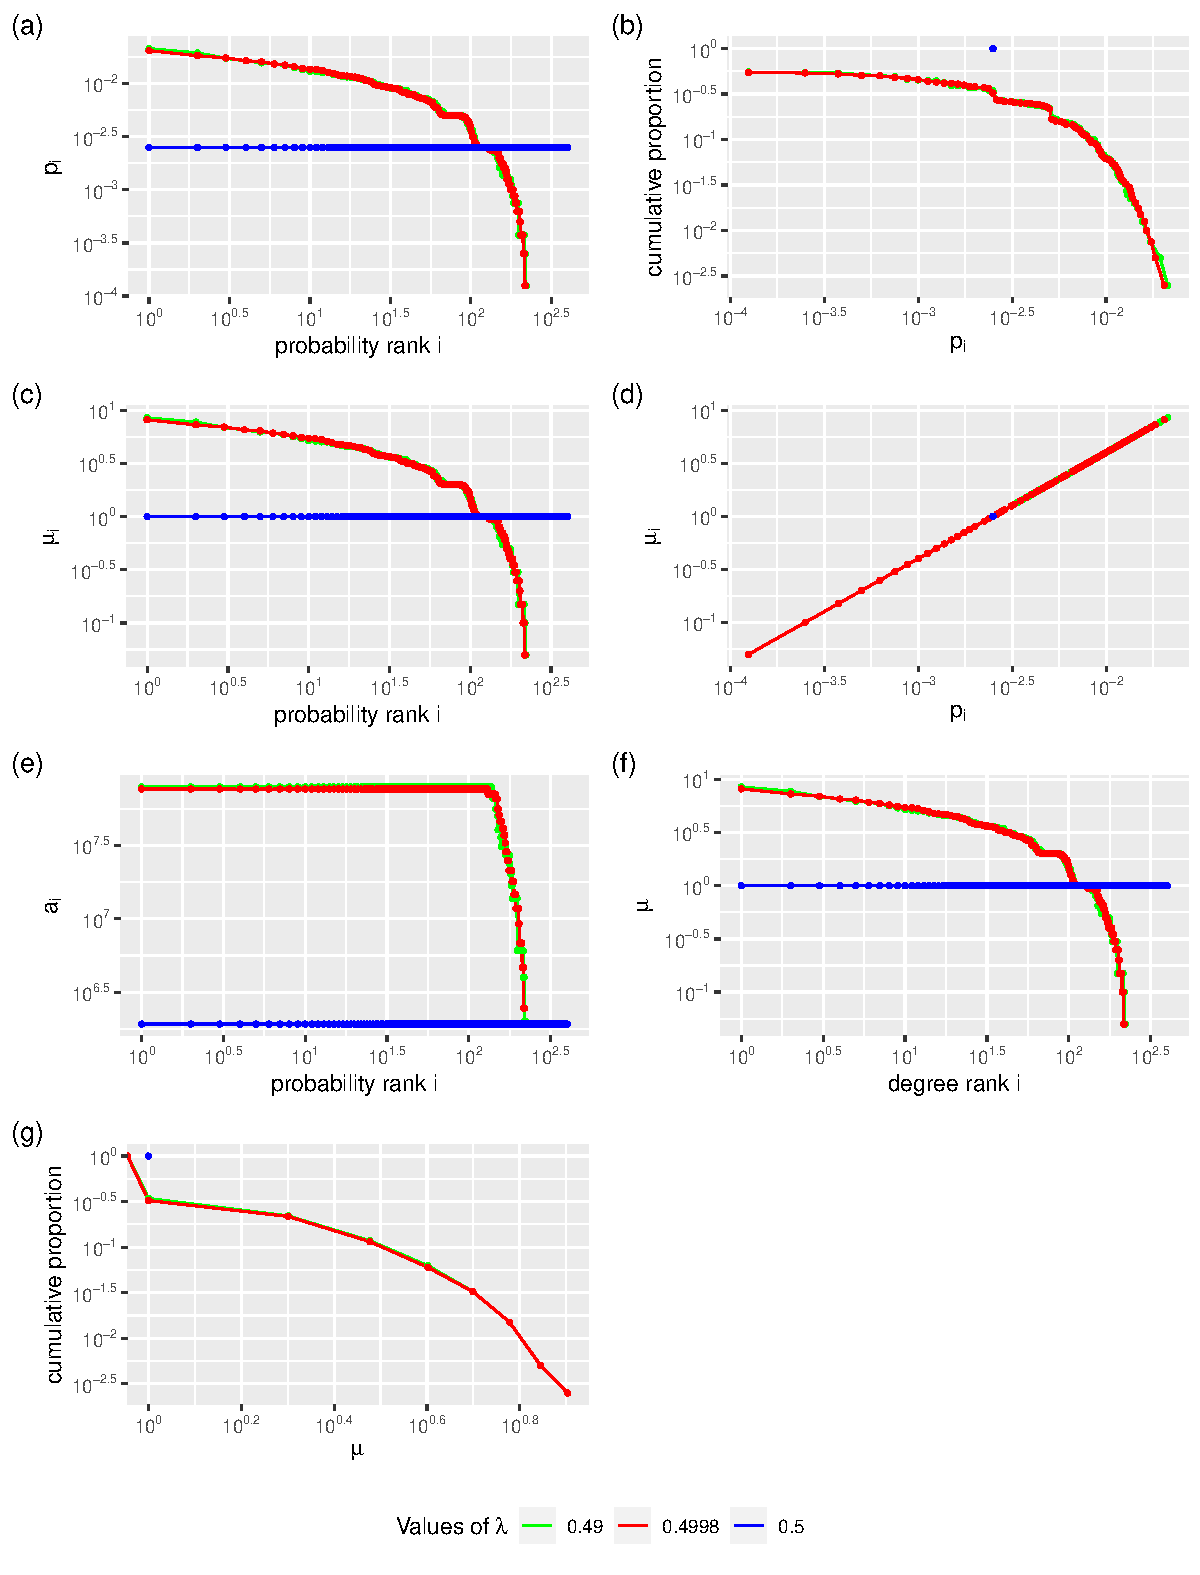
\includegraphics[width=\textwidth,draft]{insideLambda_uniform_phi1_nm400_dynamic_oneToOne_disallowUnlinked.pdf}
  \caption{a}
  \label{fig:insideLambda_uniform_phi1_nm400_dynamic_oneToOne_disallowUnlinked}
\end{figure}

all $\pi$ uniform

\begin{itemize}
\item allow disconnect meanings
  \begin{itemize}
  \item initial: random \ref{fig:insideLambda_uniform_phi1_nm400_dynamic_randomBipartite_allowUnlinked}
  \item initial: single \ref{fig:insideLambda_uniform_phi1_nm400_dynamic_singleLink_allowUnlinked}
  \item initial: one-to-one \ref{fig:insideLambda_uniform_phi1_nm400_dynamic_oneToOne_allowUnlinked}
  \end{itemize}
\item do not allow disconnect meanings
  \begin{itemize}
  \item initial: random \ref{fig:insideLambda_uniform_phi1_nm400_dynamic_randomBipartite_disallowUnlinked}
  \item initial: single \ref{fig:insideLambda_uniform_phi1_nm400_dynamic_singleLink_disallowUnlinked}
  \item initial: one-to-one \ref{fig:insideLambda_uniform_phi1_nm400_dynamic_oneToOne_disallowUnlinked}
  \end{itemize}
\end{itemize}

\subsection{Graph visualization (smaller graphs)}

\begin{figure}
  \centering
  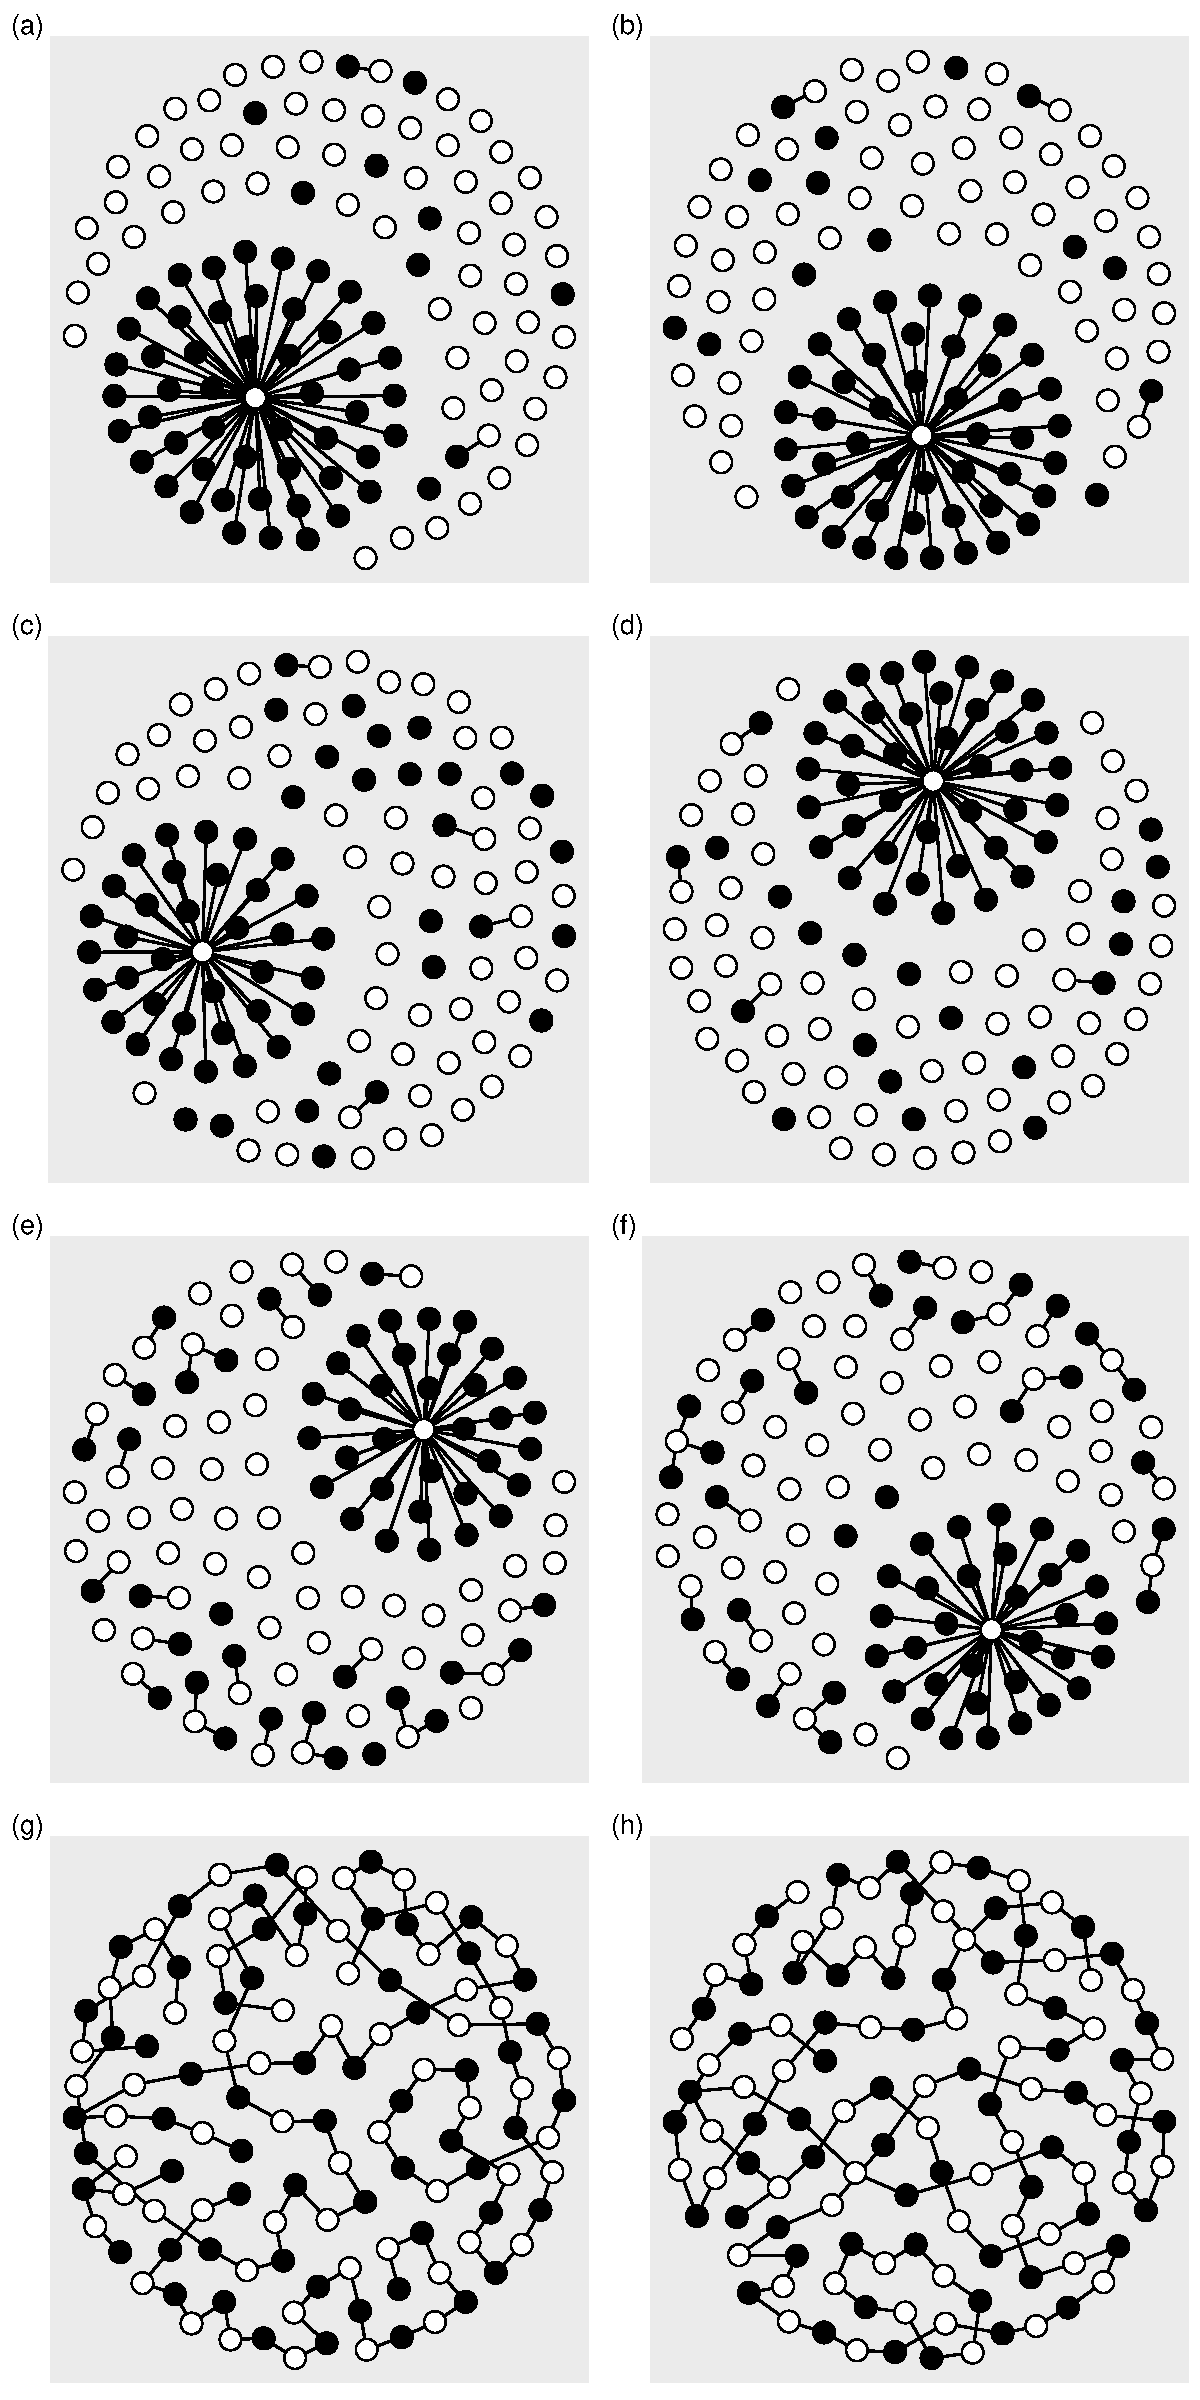
\includegraphics[height=\textheight,width=\textwidth,keepaspectratio]{graphVisualization_firstModel_phi1_nm60_static_randomBipartite_allowUnlinked}
  \caption{a}
  \label{fig:graphVisualization_firstModel_phi1_nm60_static_randomBipartite_allowUnlinked}
\end{figure}

\begin{figure}
  \centering
  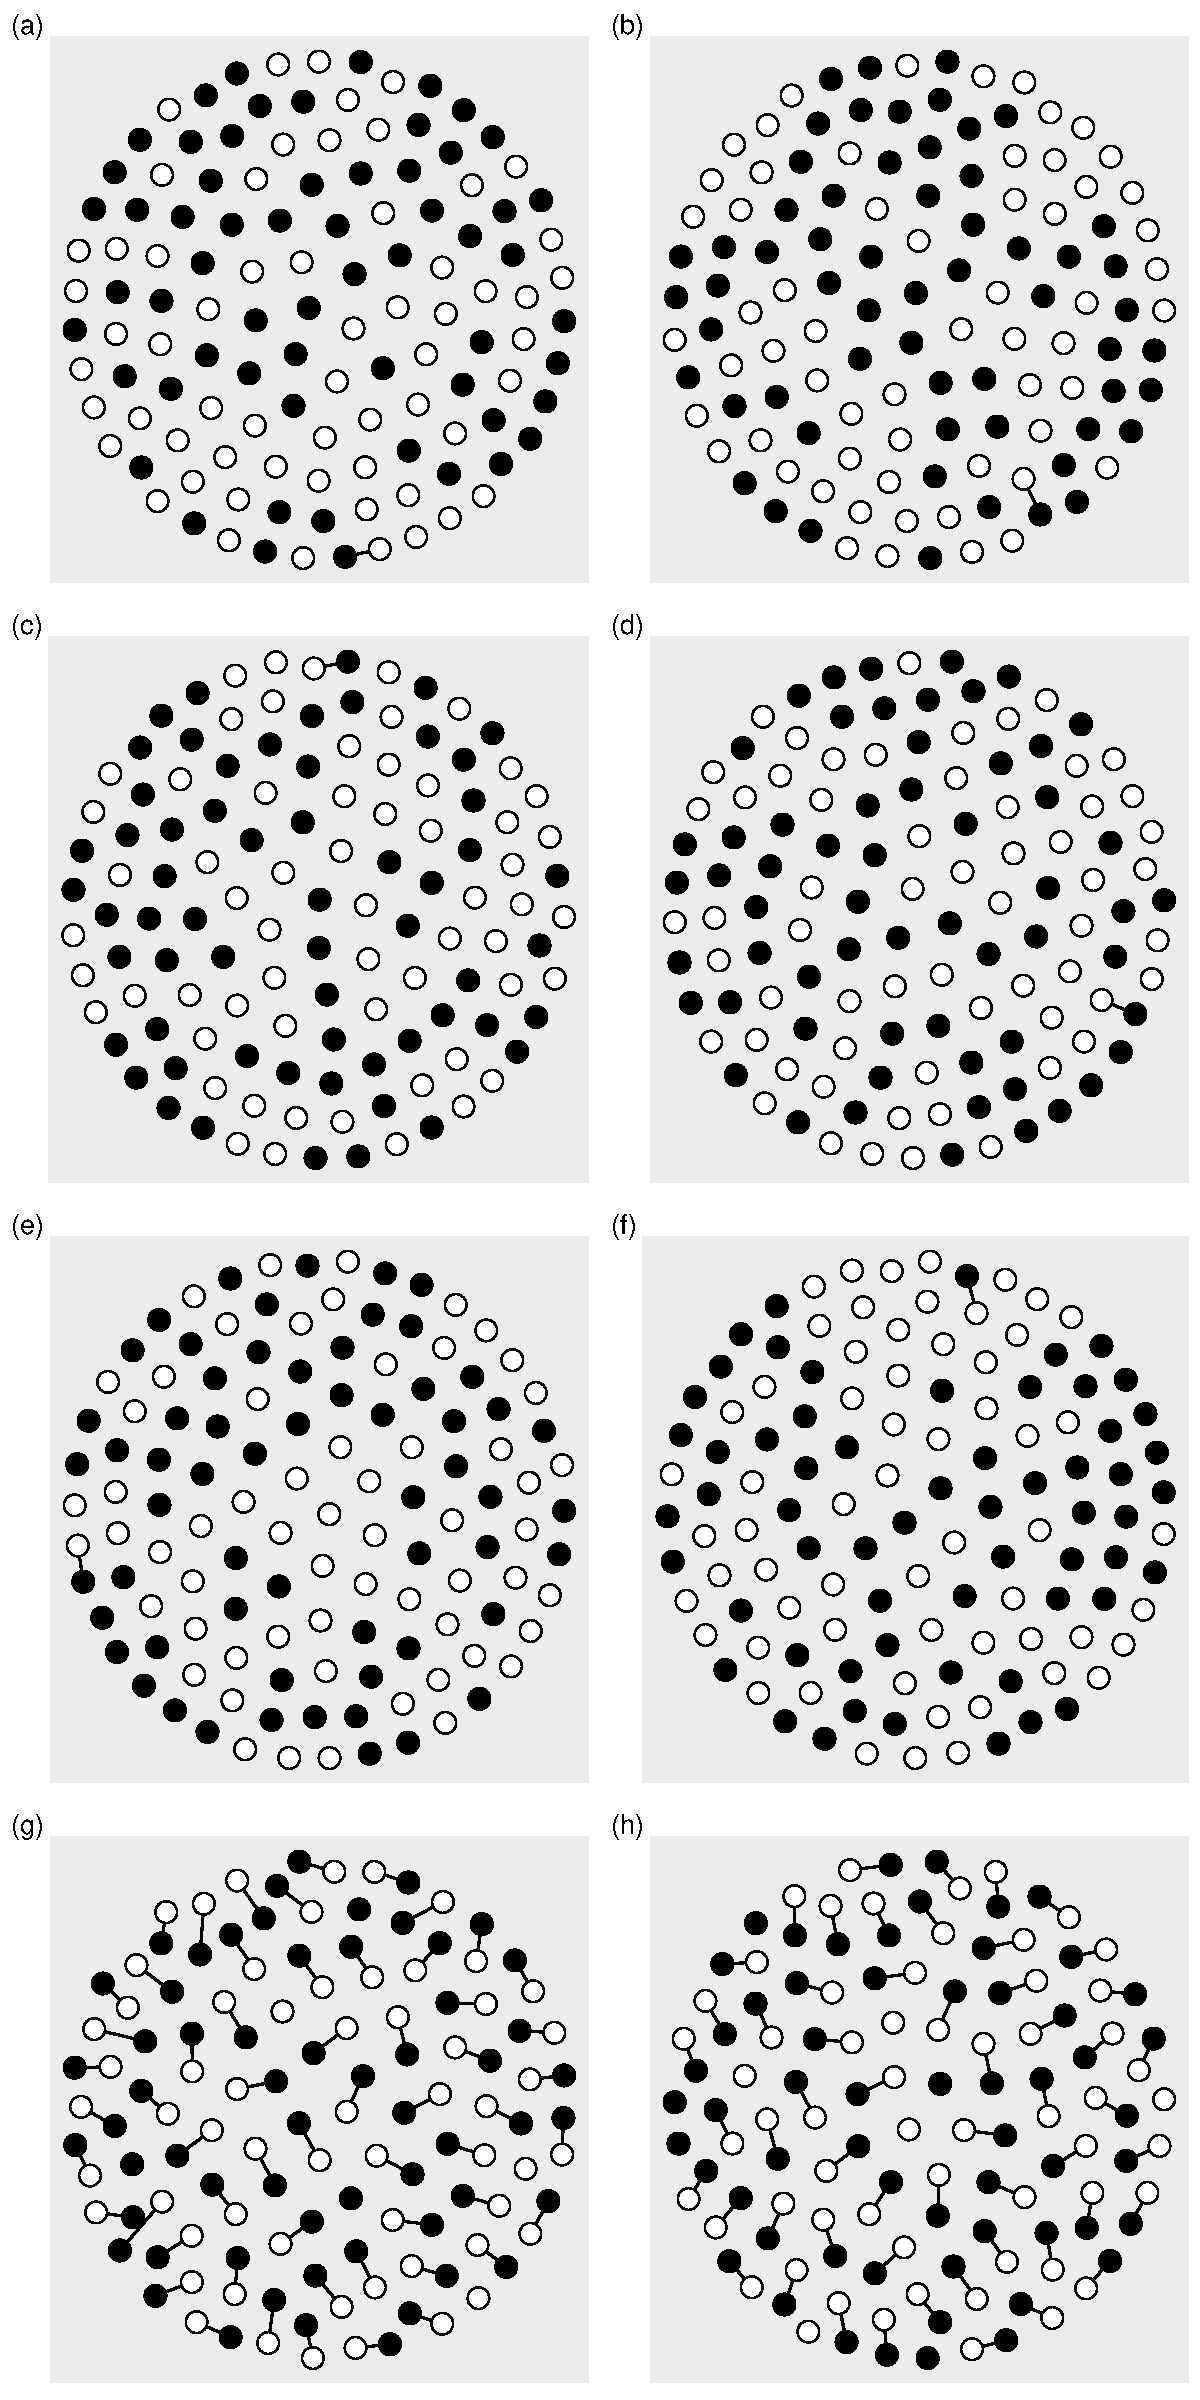
\includegraphics[height=\textheight,width=\textwidth,keepaspectratio]{graphVisualization_firstModel_phi1_nm60_static_singleLink_allowUnlinked}
  \caption{a}
  \label{fig:graphVisualization_firstModel_phi1_nm60_static_singleLink_allowUnlinked}
\end{figure}

\begin{figure}
  \centering
  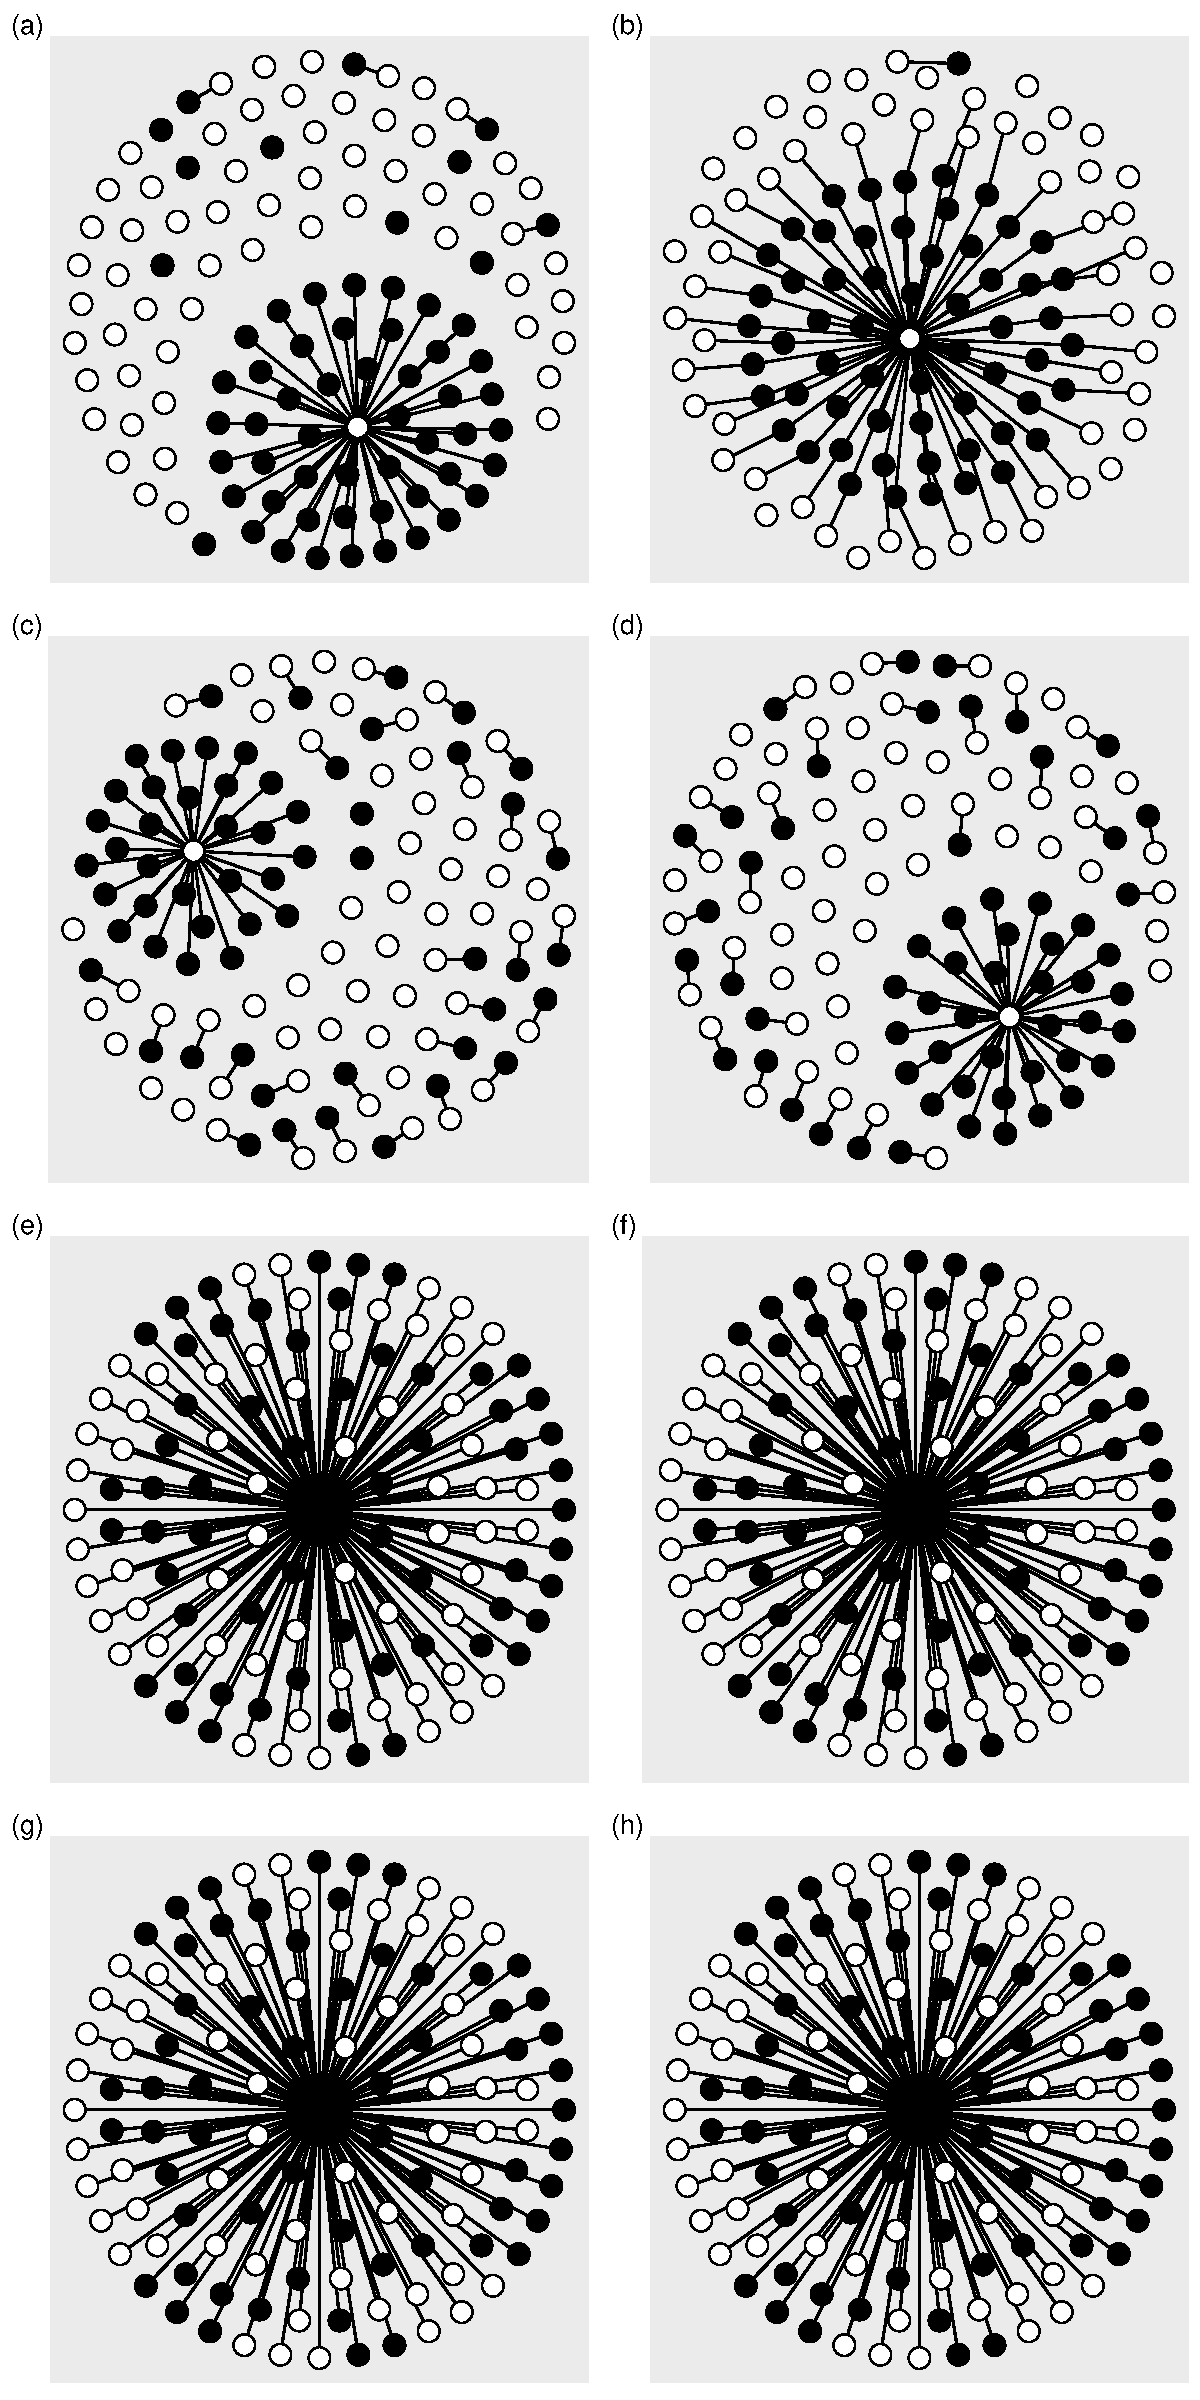
\includegraphics[height=\textheight,width=\textwidth,keepaspectratio]{graphVisualization_firstModel_phi1_nm60_static_oneToOne_allowUnlinked}
  \caption{a}
  \label{fig:graphVisualization_firstModel_phi1_nm60_static_oneToOne_allowUnlinked}
\end{figure}

\begin{figure}
  \centering
  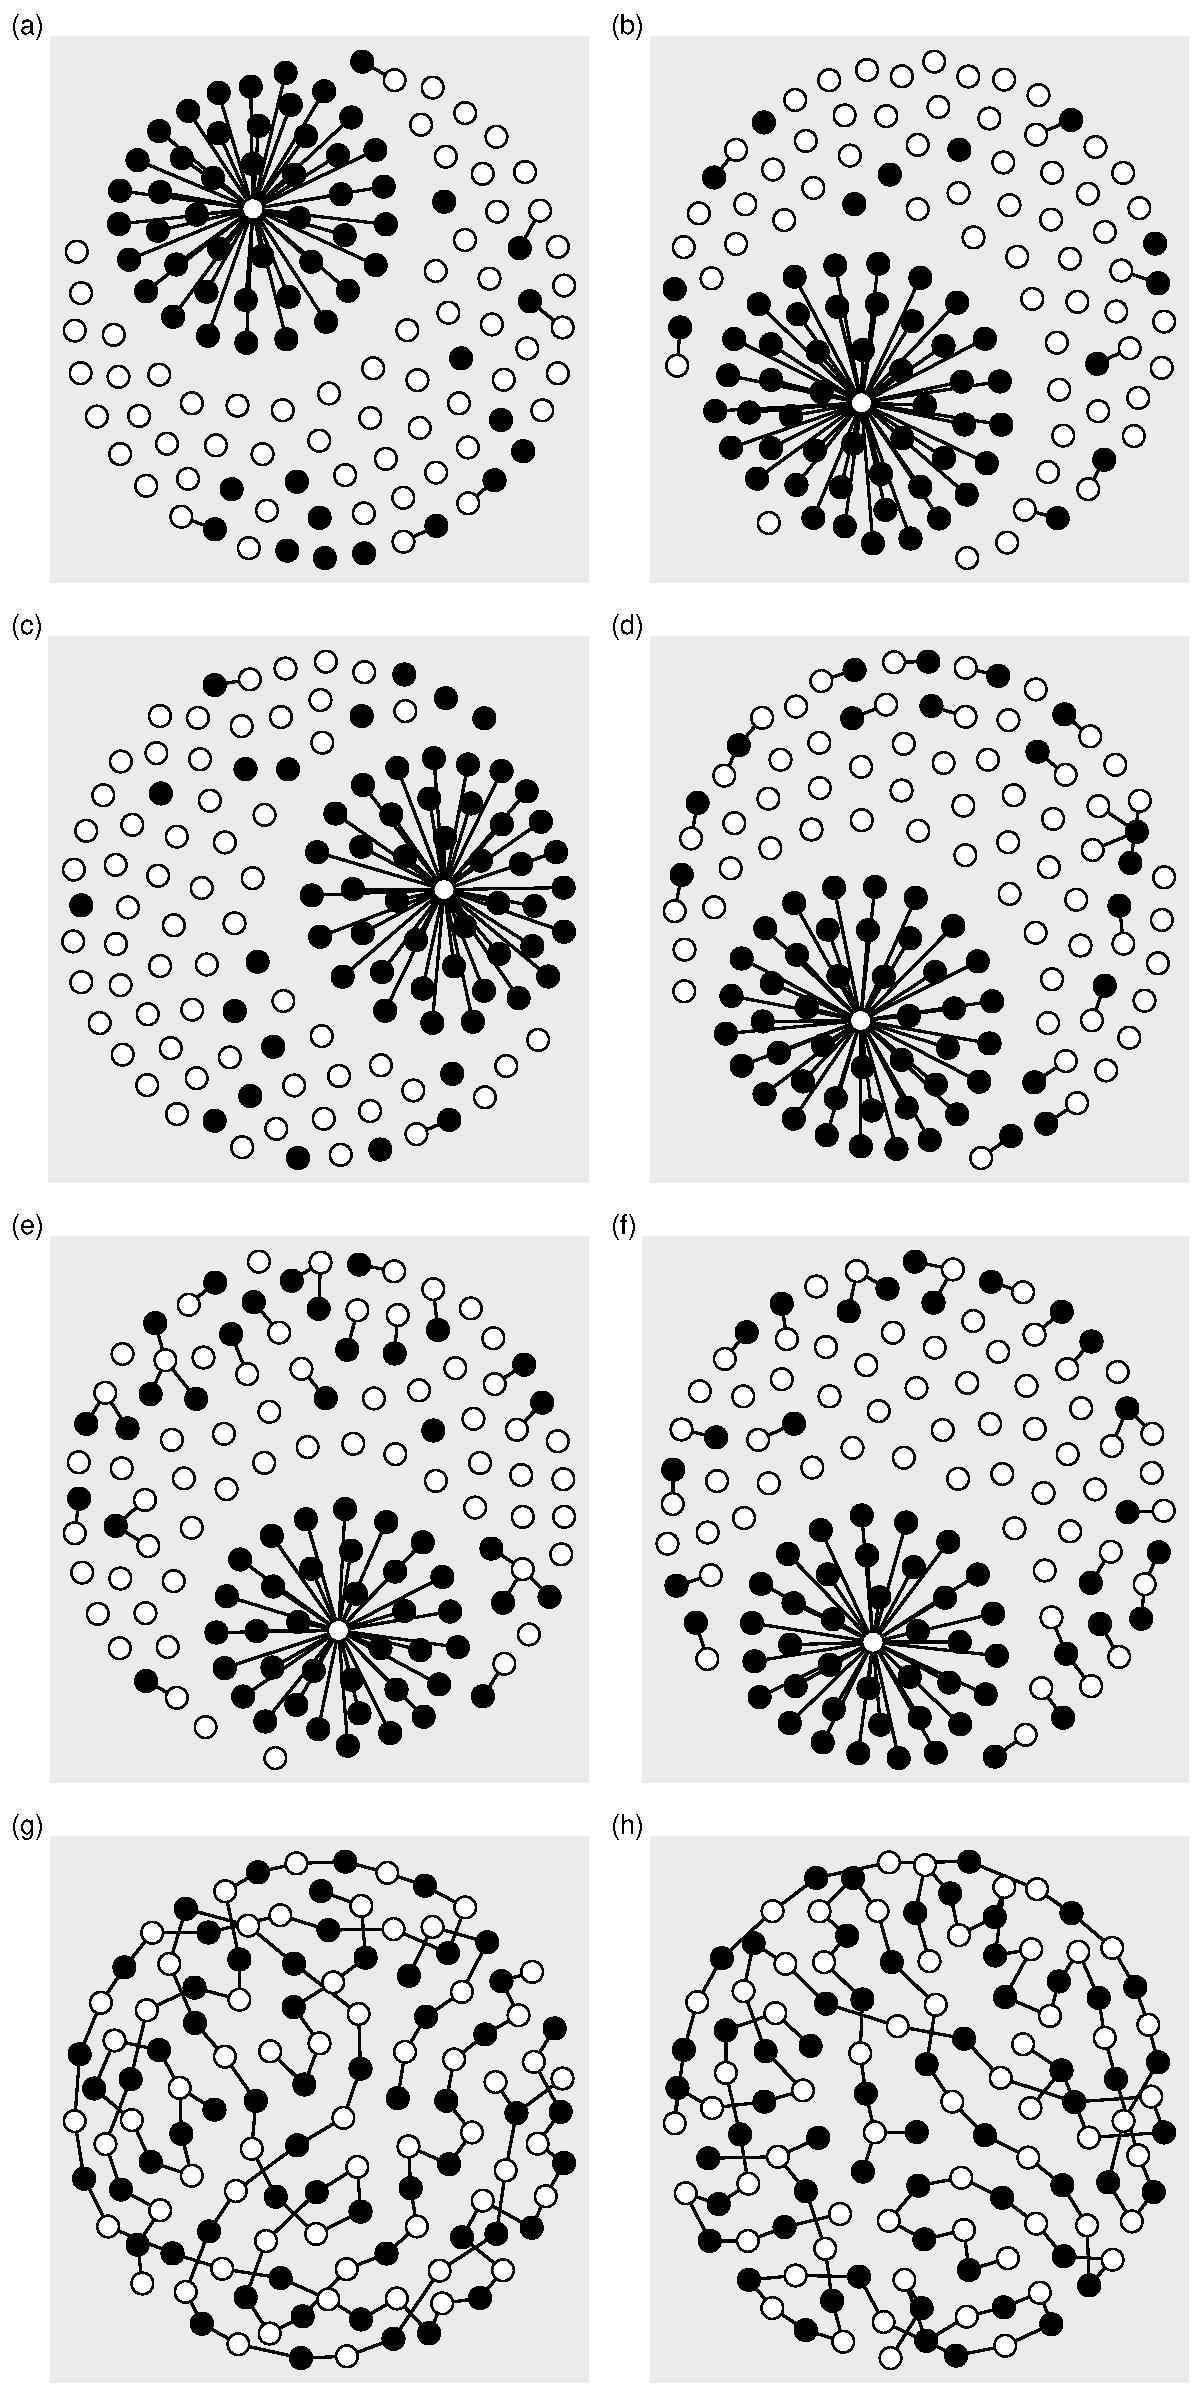
\includegraphics[height=\textheight,width=\textwidth,keepaspectratio]{graphVisualization_firstModel_phi1_nm60_static_complete_allowUnlinked}
  \caption{a}
  \label{fig:graphVisualization_firstModel_phi1_nm60_static_complete_allowUnlinked}
\end{figure}

\begin{figure}
  \centering
  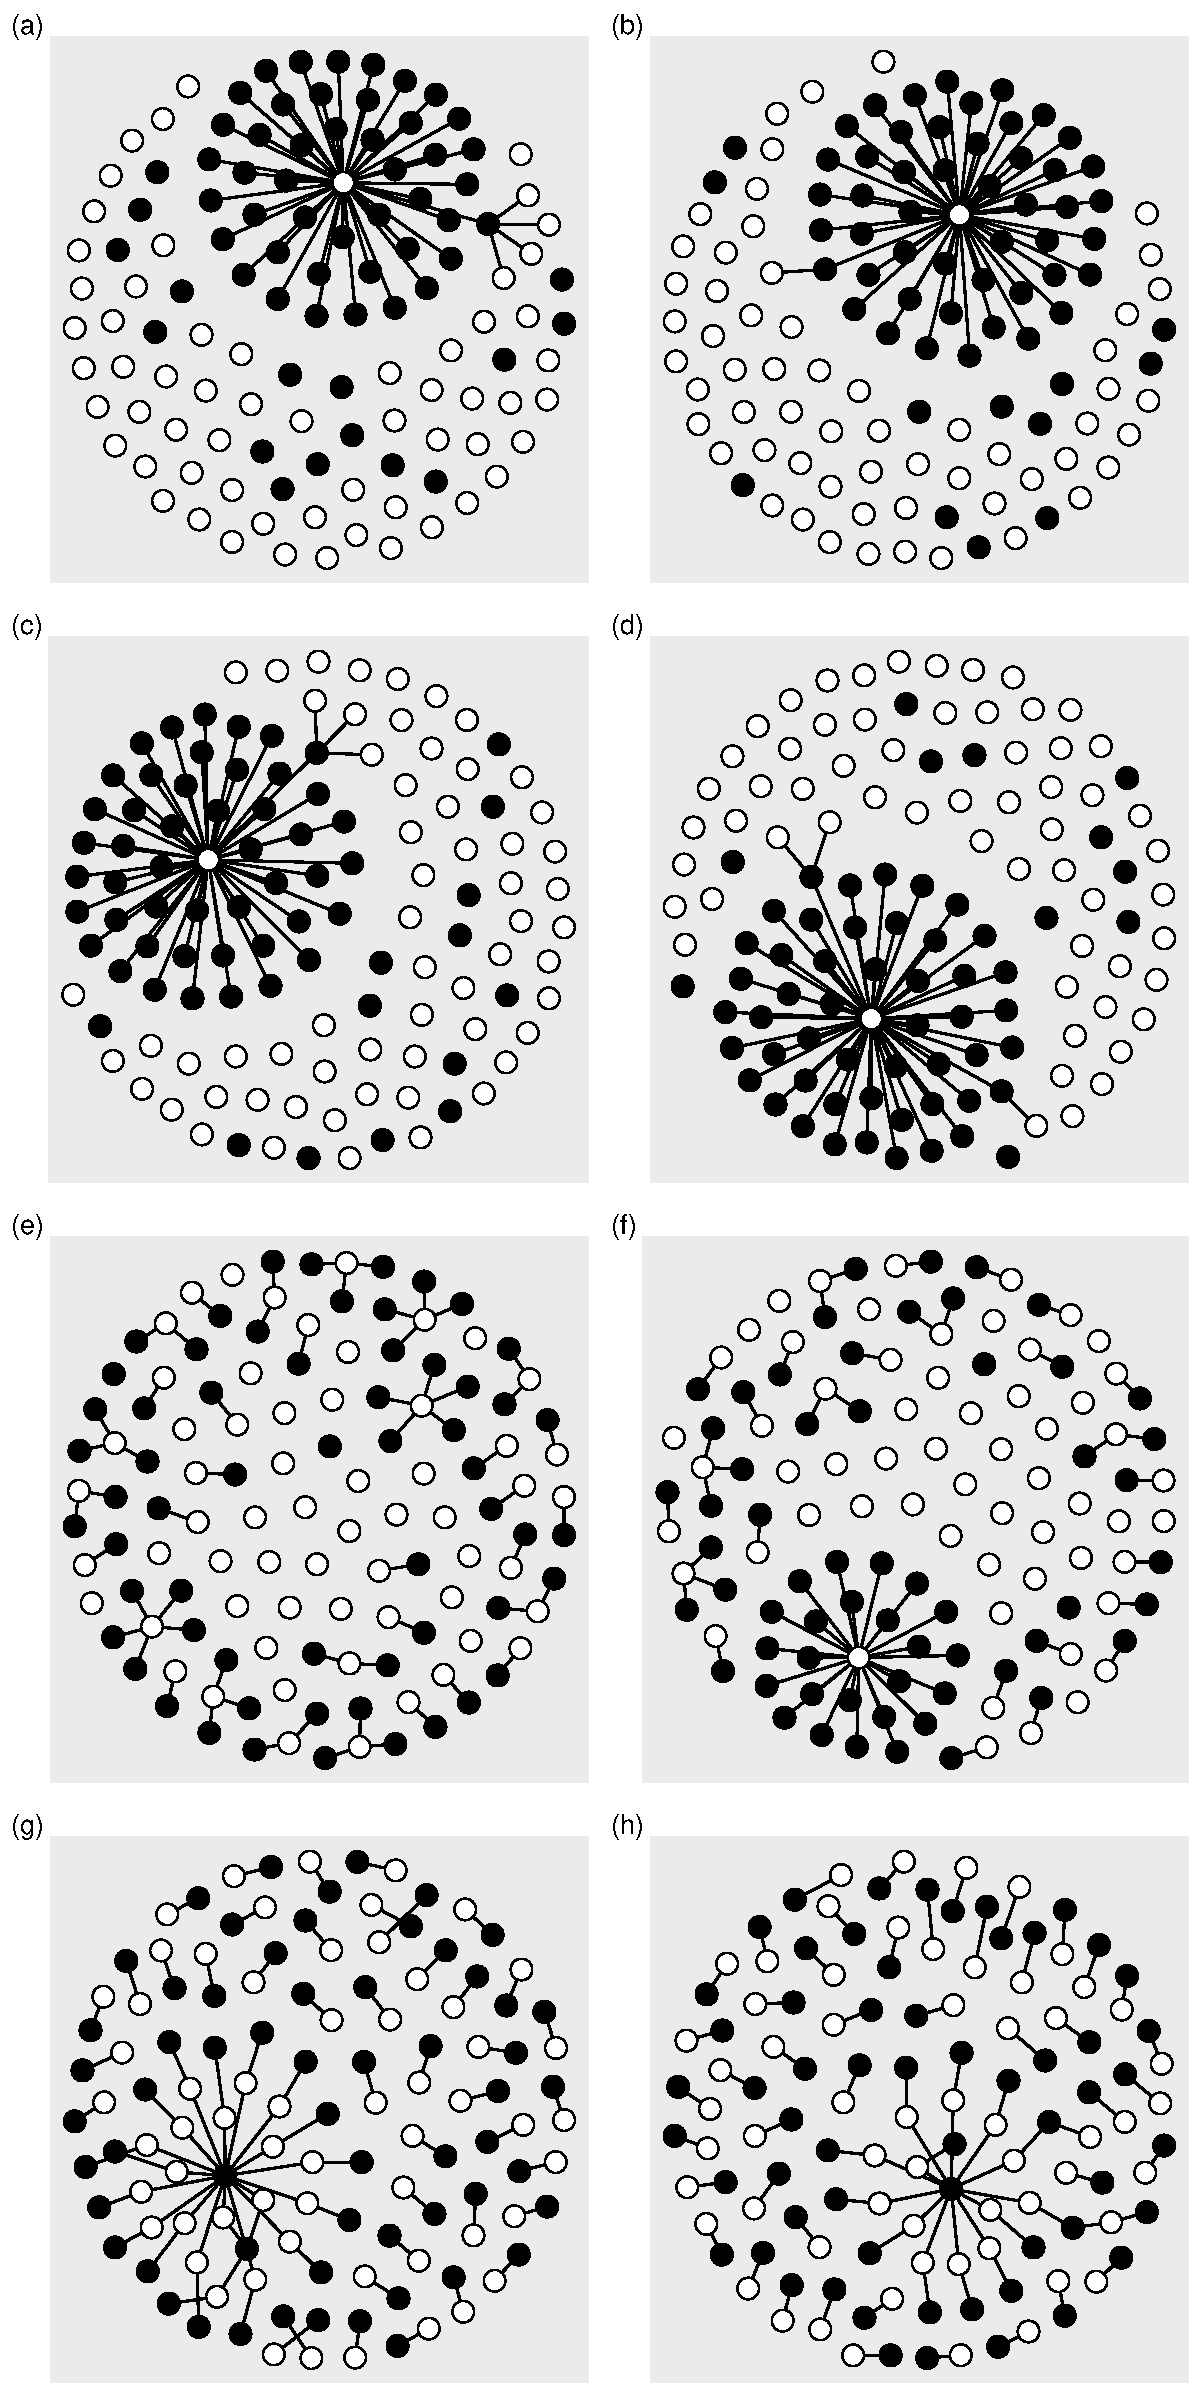
\includegraphics[height=\textheight,width=\textwidth,keepaspectratio]{graphVisualization_uniform_phi1_nm60_static_randomBipartite_allowUnlinked}
  \caption{a}
  \label{fig:graphVisualization_uniform_phi1_nm60_static_randomBipartite_allowUnlinked}
\end{figure}

\begin{figure}
  \centering
  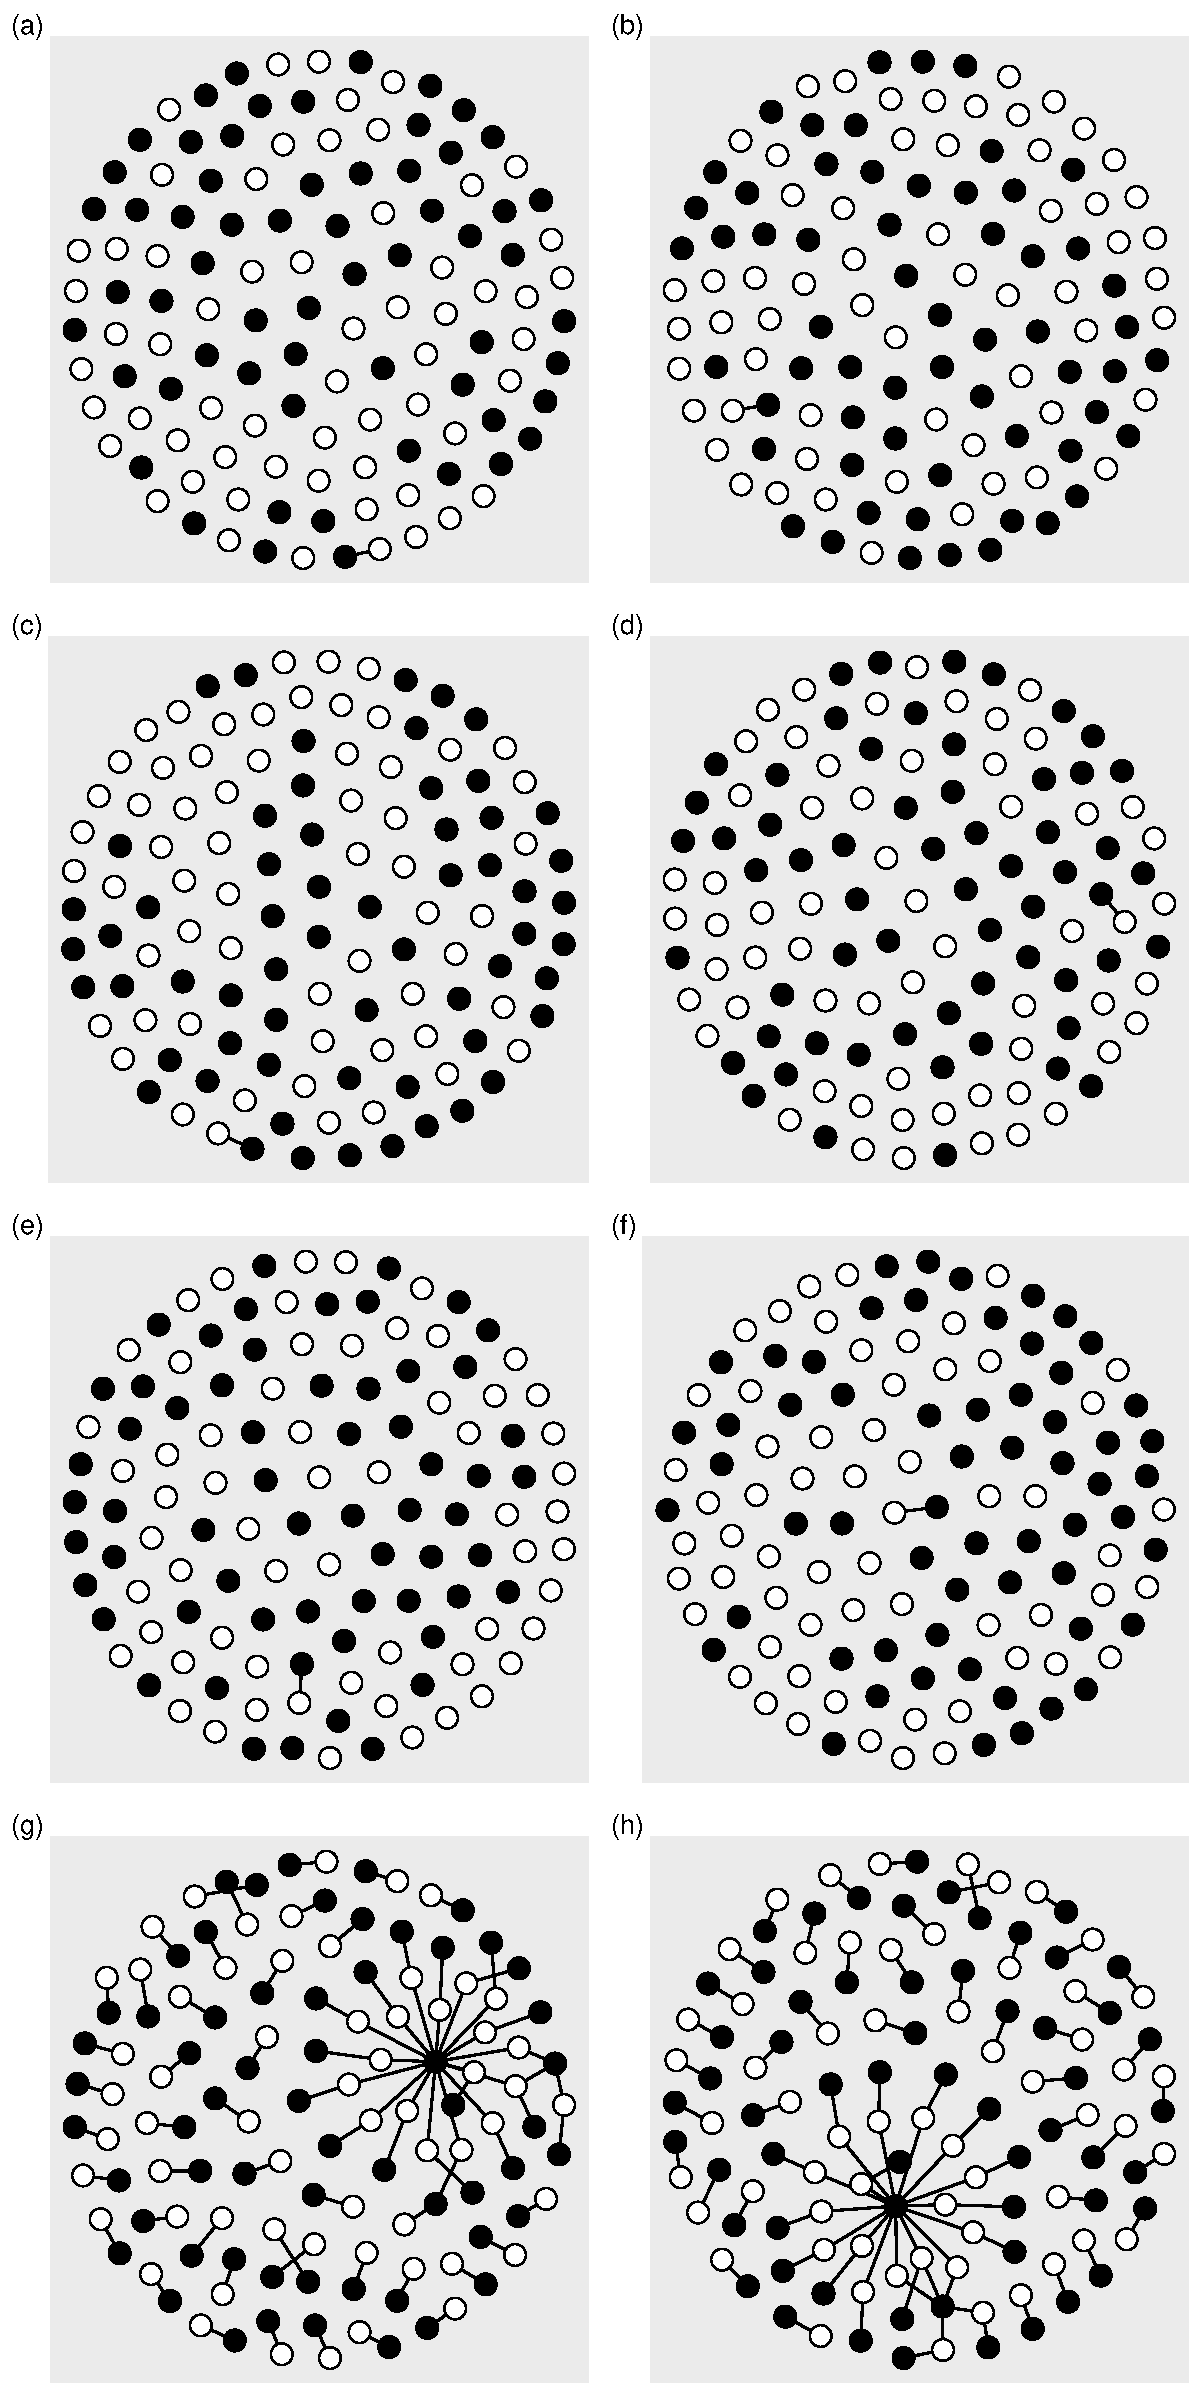
\includegraphics[height=\textheight,width=\textwidth,keepaspectratio]{graphVisualization_uniform_phi1_nm60_static_singleLink_allowUnlinked}
  \caption{a}
  \label{fig:graphVisualization_uniform_phi1_nm60_static_singleLink_allowUnlinked}
\end{figure}

\begin{figure}
  \centering
  \includegraphics[height=\textheight,width=\textwidth,keepaspectratio]{graphVisualization_uniform_phi1_nm60_static_oneToOne_allowUnlinked}
  \caption{a}
  \label{fig:graphVisualization_uniform_phi1_nm60_static_oneToOne_allowUnlinked}
\end{figure}

\begin{figure}
  \centering
  \includegraphics[height=\textheight,width=\textwidth,keepaspectratio]{graphVisualization_uniform_phi1_nm60_static_complete_allowUnlinked}
  \caption{a}
  \label{fig:graphVisualization_uniform_phi1_nm60_static_complete_allowUnlinked}
\end{figure}

all $\phi=1$

\subsubsection{first model}

\begin{itemize}
\item initial: random \ref{fig:graphVisualization_firstModel_phi1_nm60_static_randomBipartite_allowUnlinked}
\item initial: single \ref{fig:graphVisualization_firstModel_phi1_nm60_static_singleLink_allowUnlinked}
\item initial: one-to-one \ref{fig:graphVisualization_firstModel_phi1_nm60_static_oneToOne_allowUnlinked}
\item initial: complete \ref{fig:graphVisualization_firstModel_phi1_nm60_static_complete_allowUnlinked}
\end{itemize}

\subsubsection{second model}

\begin{itemize}
\item initial: random \ref{fig:graphVisualization_uniform_phi1_nm60_static_randomBipartite_allowUnlinked}
\item initial: single \ref{fig:graphVisualization_uniform_phi1_nm60_static_singleLink_allowUnlinked}
\item initial: one-to-one \ref{fig:graphVisualization_uniform_phi1_nm60_static_oneToOne_allowUnlinked}
\item initial: complete \ref{fig:graphVisualization_uniform_phi1_nm60_static_complete_allowUnlinked}
\end{itemize}


%%% Local Variables:
%%% mode: latex
%%% TeX-master: "tfm"
%%% End:
